% 元の
% \documentclass[lualatex,book,paper=a4paper,jafontsize=11.5pt,jafontscale=1.05]{jlreq}
\documentclass[lualatex,book,openany,paper=a4paper,jafontsize=11.5pt,jafontscale=1.05]{jlreq}
% 2ページ目や章の前に一ページ余分なものがあるのが気になる場合は openanyを\documentclass[...,book,openany ,..]として追加する

%フォント:
\usepackage{luatexja-fontspec}
\usepackage{hack-fonts}

%表紙用:
\usepackage{hack-cover}

\usepackage{tabularx}
\usepackage{tikz}
\usetikzlibrary{trees}
\usetikzlibrary{positioning, arrows.meta}

% FBS PBS
\usepackage{forest}
\usepackage[T1]{fontenc}
\usepackage{lmodern}

% 画像
\usepackage{float}

% 表作成用
\usepackage{array}
\usepackage{multirow}
\usepackage{graphicx}

% リンク
\usepackage[hidelinks]{hyperref}

\title{ハッカソン}
\subtitle{～計画書と設計書～}
\team{チーム26}
\author{
        24G1040 : 金枝 優介\\
        24G1074 :  荘司 あかね\\
        24G1125 : 三芝 空音\\
	25G1009 : 飯塚 蓮\\
        25G1034 : 恩田 隼士\\
        25G1063 : 佐藤 羽琉
        }
\date{\today}
\version{1.6}

%%%%%%%%%%%%%%%%%%%%%%%%%%%%%%%%%%%%%%%%%%%%%%%%
\begin{document}
\maketitle % 一ページ目

\setcounter{tocdepth}{2}
\tableofcontents \thispagestyle{empty} % 2ページ目

%%%%%%%%%%%%%%%%%%%%%%%%
%%%%%%%%%%%%%%%%%%%%%%%%
%%%%%%%%%%%%%%%%%%%%%%%%
\chapter{プロジェクトの計画書} \label{chap:project-plan}\setcounter{page}{1} % ここでページ1にしている

%%%%%%%%%%%%%%%%%%%%%%%%
\section{プロジェクトの概要}
% キーワード　マイコン　演奏　通信　役割
% 一旦どういうものを作るのかを説明(概要)
% 構成要素の役割，説明
% 最終的な動作　構成要素をどうやって接続しシステムを構築すると考えているの
% 本プロジェクトでは，Arduinoの制御に基づく楽器間同期演奏システムの構築を目的とする．
% 本システムは，指揮者としてのArduino，演奏者としての複数のArduino，および，楽器としての音色再生のProcessingによって構成される．
% 指揮者用のArduinoは，楽曲のテンポや音の強弱の演奏情報を信号として，各演奏者用のArduinoへ送信する．
% 演奏者用のArduinoは，受け取った演奏情報と内部の楽譜情報に基づき，Processingへ演奏内容を送信することで音の再生を行う．
% 送信された信号に基づき，演奏者用のマイクロコントローラは楽譜の役割として再生する音階，長さなどの情報を楽器としてのProcessingへのプログラムに渡し，演奏を行う．
%  本演奏システムでは，指揮者としてのArduino，楽譜や演奏者としての複数台のArduino，そして，楽器として演奏者のArudinoに接続されたProcessingによる音の再生によってオーケストラを作成する．
\subsection{プロジェクトの題目}
% 独自性のアピールポイント?
% 何がこのプロジェクトとして目指すものか
% 今回は同期処理かな
% 題目が指している技術・対象の説明
% 何を主軸にしたプロジェクトなのか
% キーワードの定義 同期など
% 〇〇の検討
% 研究対象 + アプローチ + コア技術
% 同期演奏システム　Arduino間制御  指揮者モデル
本プロジェクトの題目は，「単一のフルカラーLEDとArduinoを用いた光無線通信による楽器間同期演奏システムの開発」である．
%%%%%%%%%%%%%%%%%%%%%%%%
\subsection{プロジェクトの目的}
% プロジェクトの目的と最終的なゴール，解決すべき課題を記述する．
% なぜそれを目的としたのか or 解決すべき課題(参考文献) -> 何を作るのか(独自性のフォーカスポイント) -> 最終的に何を目指すのか 
% 自動演奏システム，同期信号についてなんであるのか，どんな種類があるのか，またそれらの問題 (社会的，技術的背景)
% 同期演奏についての問題か同期システムとしての問題か
% 解決すべき課題からこの同期演奏システムでどういった同期処理を行うことでアプローチ(方法時代は既存のでもいい)できるのか．
% 最終的にどこを目標とするのか
従来の同期システムでは，有線接続による配線制約や，無線通信における通信遅延・通信環境依存などが課題となっている．
本プロジェクトの目的は，LEDの光を用いた無線通信による楽器間同期演奏システムを構築し，楽器演奏のズレを最小限に抑え，合奏を成立させることである．
さらに，利用者が楽器変更やテンポ変更等の演奏機能を制御するためのWebサイトや視覚的に合奏を認識するためにLEDマトリクス歌詞表示システムを構築することでシステムの操作性及びエンターテイメント性の向上を目指す．
最終的なゴールは，ユーザの操作に応じて，複数楽器の同期演奏を成立させることである．
% こういう課題を見つけて問題解決するということは社会で必要となってくるが，最初は大きな方針(何するか)を決めて，それに対しての課題を見つけることに苦労しているので
% 参考文献として同じような問題に対してどういったアプローチをとているのがあるかを提示して読み込ませてから，問題解決などの方法について話し合いをしたほうが学習のパターンかとして
% 効果があるのではないか．
%%%%%%%%%%%%%%%%%%%%%%%%
\section{社会的背景}
近年，音楽演奏や視覚演出の分野において，出力装置を複数台組み合わせた作品やシステムが研究されている．
例えば神田らは複数のモバイルデバイスを用いたインタラクティブメディアアートを提案している\cite{組み合わせ}．
これらのシステムでは，各装置が正確なタイミングで動作することが求められ，リアルタイム同期処理が重要な要素となる．


特に音楽演奏においては，複数の演奏者や演奏装置が同一テンポで動作する必要があり，わずかな同期ズレであっても演奏品質に影響を与える．
音声遅延が演奏に与える影響は大きく，先行研究では数ms程度の遅延であっても演奏品質や演奏感覚に影響を与えることが報告されている\cite{遅延研究}．
そのため，演奏同期システムにおいては，演奏に支障を与えるような遅延や同期ズレを低減するための高精度な同期制御技術が求められる．


また，近年のIoT技術の発展により，様々なデバイスがネットワークに接続されるようになり，
データ流通量のさらなる増加へとつながっている\cite{IoT}．
このような技術は，スマートホームや産業機器の制御，エンターテインメントシステムなど，
多様な分野において応用されている．


一方で，複数装置を連携させる従来の同期システムでは，有線接続による配線制約や，無線通信における通信遅延・通信環境依存などの課題が存在する．
そのため，複数装置を柔軟に同期可能な，新たな同期手法が求められている．


また，輪唱のような複数パートが異なるタイミングで演奏する楽曲では，聴衆が各パートの演奏状況を聴覚のみで把握することは難しい．
音楽演奏において視覚情報と聴覚情報を組み合わせることで，聴衆の楽曲理解や没入感が向上することが報告されており\cite{視覚聴覚}，演奏システムに
おける視覚的演出の重要性は高まっていると言える．

\subsection{既存の技術とプロジェクトの独自性}
% 目的(問題)に対しての既存技術を調べる
% そこから何か新しい視点がないかを探して独自性とする

既存の通信方法として現在幅広く利用されているものに，有線通信およびBluetoothやWi-Fiを用いた無線通信がある．

有線通信は通信の安定性が高く遅延の影響を受けにくいという利点を持つが，複数装置を接続するためには配線が必要となり，設置の自由度が低下するという課題がある．
特に近距離環境での複数装置の同期において，配線の取り回しがシステム構成の複雑化を招く．
一方，無線通信は配線を必要とせず柔軟なシステム構成が可能であるが，電波干渉や通信環境の影響を受けやすく，遅延やパケット損失が発生する可能性がある\cite{無線}．


また，本システムに関連する技術として光無線通信が挙げられる．
光無線通信とは，我々が日常的に使用している放送や携帯電話の電波と同じ電磁波の一種である光を電波媒体とするシステムである\cite{光無線通信}．
この通信システムの光源にはLEDやLD， VCSELが用いられ，光信号の受信用検出器にはPin-PDやAPDが使われる．


従来の光通信では，光の有無や強弱といった単一の情報を扱う方式が一般的であり，伝達可能な情報量が限られるという課題がある．
これは，従来の強度検出型の光通信方式では，主に光の強弱のみを情報として利用していることに起因する．
また，外乱光の影響を受けやすく，環境光の変動による誤検出が生じる可能性がある．
さらに，複数の信号を識別することが困難であり，多数の装置を同時に制御する用途には適していない．



これらの課題に対し，本システムは近距離環境での複数装置の同期制御を対象とし，フルカラーLEDとカラーセンサを用いた光通信を採用することで配線を不要とし，近距離環境における配線削減およびシステム構成の簡略化を図る．


単一のLEDから全演奏者へ同時に信号を送信する構成とすることで，演奏者間の信号のばらつきをなくし，同期ズレを防ぐ設計とした．
光は電波と比較して外部からの干渉を受けにくく，混線が生じないため，無線通信で問題となる同期ズレの低減が期待される．
また，光通信ではネットワークを介した無線通信と異なり，パケット損失や通信環境変動の影響を受けにくく，安定した信号伝達を行うことができると考えられる．
加えて，単一のLEDを使用することで，有線通信のように装置の増加に伴って分配器やケーブルが増大する問題がなく，受光可能範囲内であれば装置の追加や配置変更が容易である．
さらに，光通信はネットワークを介した無線通信と比較して，通信処理が単純であるため，低遅延化が期待できる．
加えて，センサ周辺を遮光することで外部照明の影響を低減し，誤検出の低減を図る．

本システムではフルカラーLEDとカラーセンサを用いることで，光の色，発光間隔，光強度といった複数のパラメータを同時に利用した通信を実現している．
これにより，従来の強度ベースの光通信と比較してより多くの情報を表現可能である．
さらに，光の点灯間隔をセンサで検出することでテンポ情報を直接取得し，数値データを用いずに演奏タイミングを制御する点に特徴がある．
また，色ごとに異なる意味を割り当てることで複数の楽器や制御信号を同時に扱うことができる．


以上より，本システムは光通信の簡易性と多機能性を両立した光同期システムである点に独自性がある．
さらに，本システムではLEDマトリクスによる歌詞表示機能を実装することで，輪唱における各パートの演奏タイミングを視覚的に提示し，
聴覚情報のみでは把握しにくい輪唱の構造を視覚情報と組み合わせて表現する点にも独自性がある．
%%%%%%%%%%%%%%%%%%%%%%%%
%%%%%%%%%%%%%%%%%%%%%%%%
\section{スコープ・マネジメント}
%%%%%%%%%%%%%%%%%%%%%%%%

\subsection{成果物}
本プロジェクトにおける最低限達成すべき機能として，光無線通信による楽器間の演奏ズレが限りなく少ない合奏機能を実装する．
同期通信，演奏制御，エンターテイメントとしての歌詞表示を含めた本プロジェクトの成果物は，以下の通りである．
\begin{itemize}
\item フルカラーLEDを用いた光通信による同期演奏システム
\item 各楽器の音再生プログラム
\item LEDマトリクスによる歌詞表示機能
\item Web演奏制御機能
\end{itemize}
%%%%%%%%%%%%%%%%%%%%%%%%
\subsection{プロジェクトの対象範囲と非対象範囲}
フルカラーLEDを用いた同期演奏システムを構築するために必要な本プロジェクトの対象範囲は以下の通りである．
\begin{itemize}
\item LEDによる光通信機能実装
\item カラーセンサを用いた光信号の受信，解析
\item テンポ取得
\item 4種類の楽器音再生
\item Webからのテンポ変更，楽器変更，音量変更，楽譜選択・ループ演奏選択機能実装
\item LEDマトリクスによる歌詞表示
\end{itemize}


一方で，本プロジェクトでは，指揮者，演奏者間の同期通信に焦点を当てるため，実際の楽器を演奏するのではなくデータとして楽器を演奏する．
また，Webサイトでの演奏制御は同期処理に負荷をかけないよう，演奏前に楽器の変更などを行うためネットワーク環境の整備は本プロジェクトでは対象外とした．
よって，非対象範囲は以下の通りである．
\begin{itemize}
\item 商用レベルの高速・長距離光通信
\item 実際の楽器を演奏するための入力インターフェース
\item システム運用に必要なネットワーク環境の整備
\end{itemize}
%%%%%%%%%%%%%%%%%%%%%%%%
\subsection{機能分解構造FBS}
本システムのユーザ目線から見た機能分解としてのFBSを図\ref{fig:fbs}に示す．
ユーザが可能な制御は演奏中と，演奏前の二つに分けられる．
演奏前は，演奏者ごとに楽器変更，楽譜選択，個別音量の調節が可能で，演奏中は，テンポ変更，全体音量の調節，およびループ演奏の切り替えが可能である．
また，それらの演奏制御は物理的なスイッチ以外に，Webサイトを通じても行うことができる．
エンターテイメントとしては，各楽器用のArduinoのLEDマトリクスに演奏中の歌詞を表示する．
\begin{figure}[H]
  \begin{center}
    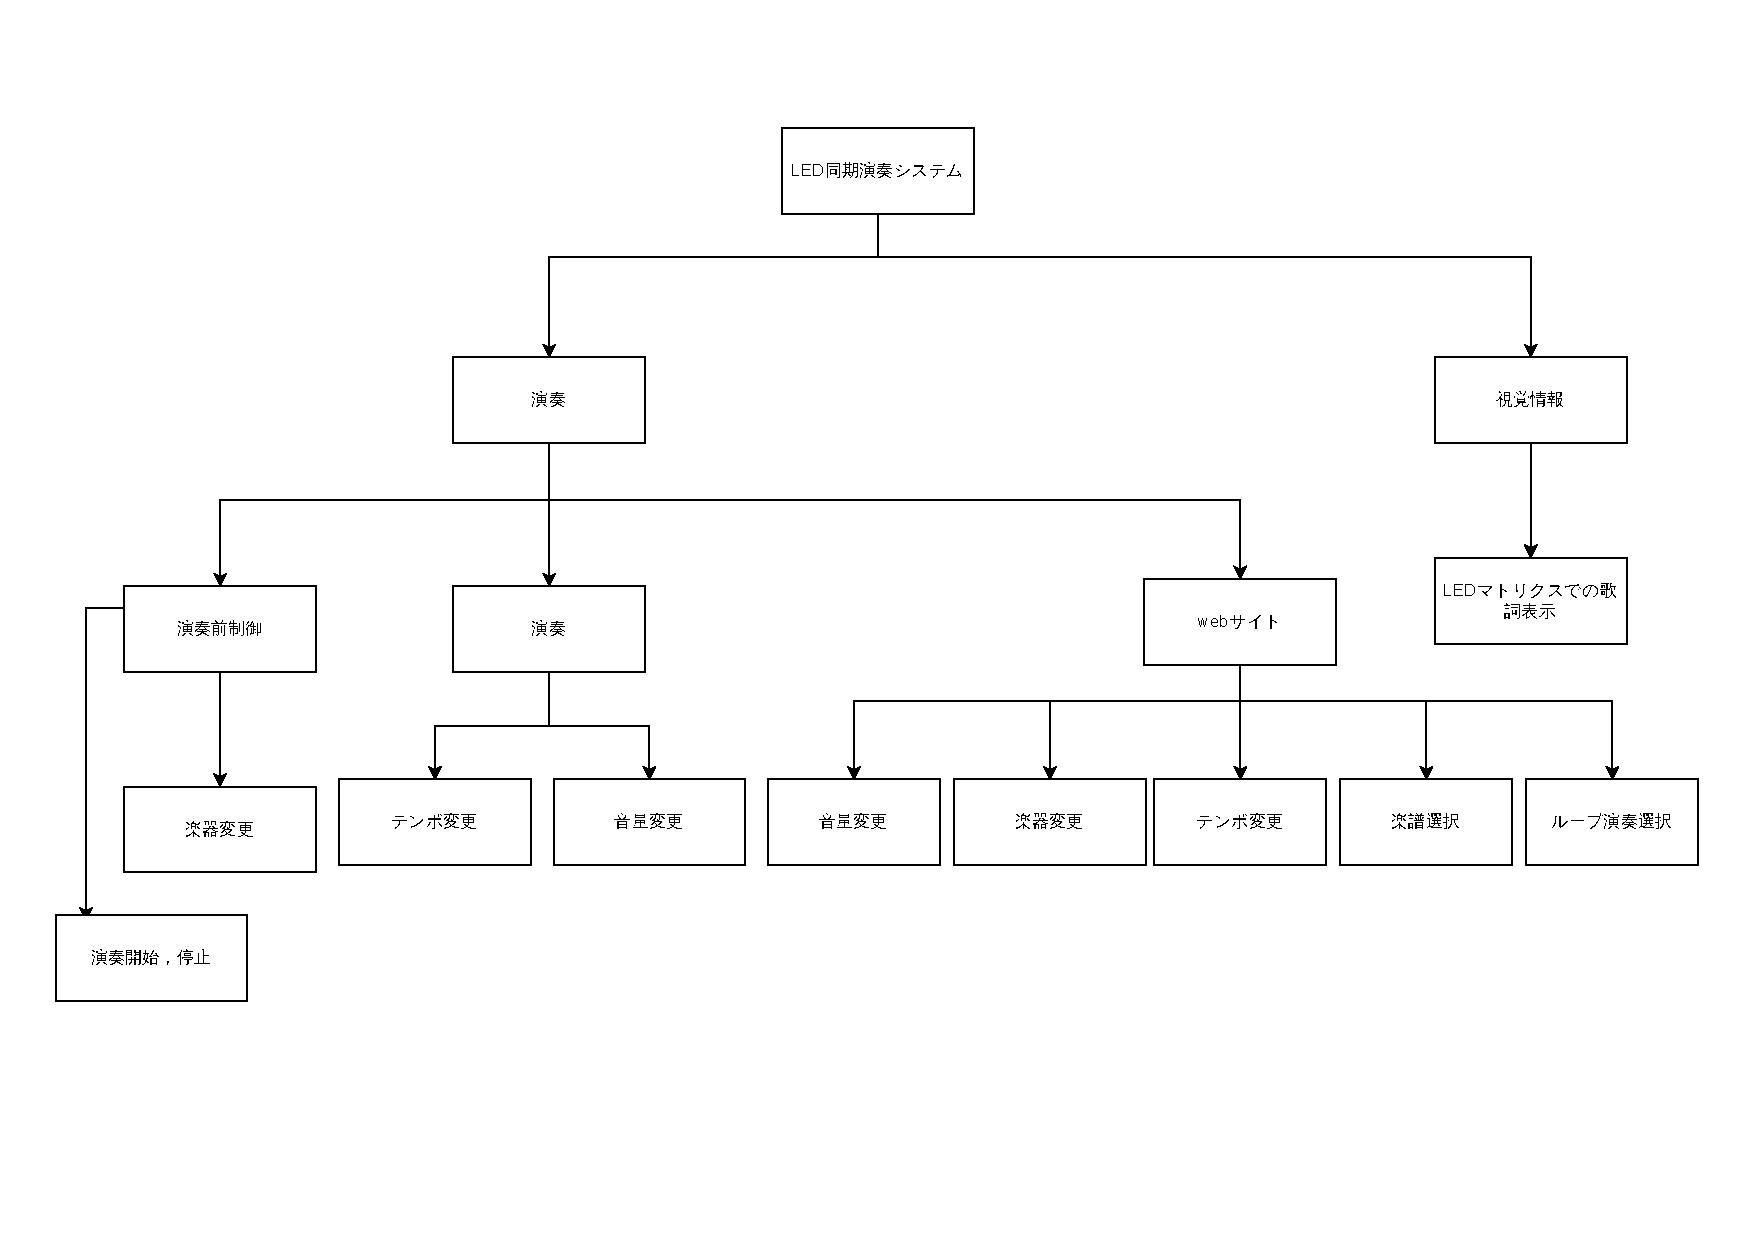
\includegraphics[width=120mm]{./img/fbs_7_1.pdf}
    \caption[FBS]{機能分解構造(FBS)}
    \label{fig:fbs}
  \end{center}
\end{figure}
%%%%%%%%%%%%%%%%%%%%%%%%
\subsection{製品分解構造PBS}
本システムのFBSを実装するための機能であるPBSを図\ref{fig:pbs}に示す．
ハードウェアの面では，演奏同期のためのLEDの送受信の機能と，演奏開始や停止などの演奏制御をボタン，スイッチを用いて実装する．
また，ソフトウェアの面では，演奏を実現するための楽器音，楽譜，歌詞のデータベース及び，制御のためのwebページを実装する．
\begin{figure}[H]
  \begin{center}
    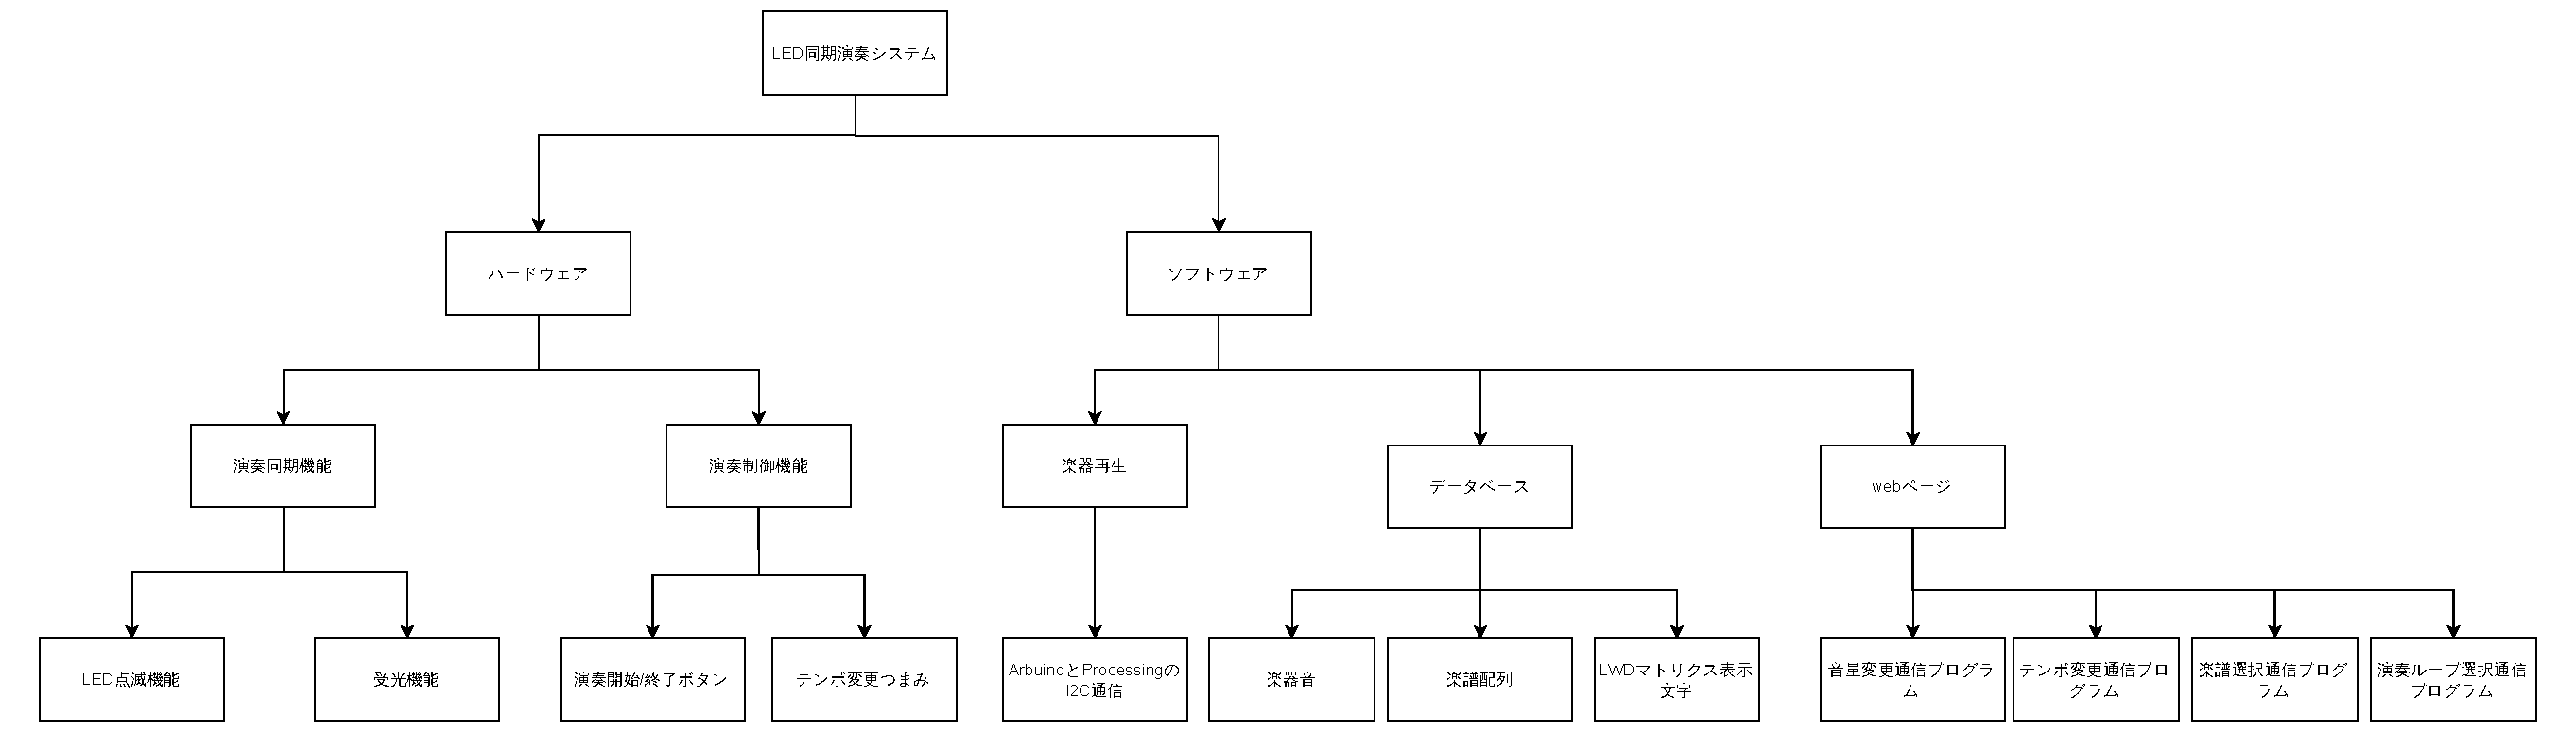
\includegraphics[width=140mm]{./img/pbs_7_3.pdf}
    \caption[PBS]{製品分解構造(PBS)}
    \label{fig:pbs}
  \end{center}
\end{figure}

%%%%%%%%%%%%%%%%%%%%%%%%
\subsection{FBSとPBSの対応関係}

FBSとPBSの対応関係を以下の表\ref{FBS_PBS}に示す．
FBSの各機能に対して，それを実現するPBSのサブ成果物を対応付けた．
各機能は1つ以上の成果物によって実現される．

「楽器演奏」機能については，ソフトウェア側の「演奏プログラム（ピアノ・バイオリン・フルート・パーカッション再生）」と，ハードウェア側の「音再生用PC」によって実現される．
「演奏制御」機能のうち，「演奏同期」は「送受信プログラム」と「フルカラーLED」「カラーセンサ」の組み合わせにより，光無線通信として実装される．
また，「演奏開始・停止」は「Webサイト」と指揮者Arduinoに設置された「タクトスイッチ」がその役割を担う．
「Webサイト」による「テンポ変更」「音量変更」「楽器変更」「楽譜選択」「ループ演奏選択」は，Webサイトに対応した各プログラムの構築により実現される．
「視覚情報表示」機能である「LEDマトリクス歌詞表示」は，ソフトウェア側の「LEDマトリクス表示プログラム（文字配列データ）」と，ハードウェア側の「演奏者Arduino」によって実装される．
このように，本プロジェクトにおける全ての機能要件は，定義されたソフトウェアおよびハードウェアの構成要素によって網羅されている．

\begin{table}[H]
\centering
\caption{FBSとPBSの対応関係}
\label{FBS_PBS}
\resizebox{\textwidth}{!}{
\begin{tabular}{|l|l|} \hline
FBS（機能） & PBS（成果物） \\ \hline
ピアノ演奏 & 演奏プログラム（ピアノ音再生），楽器音データ，楽譜配列データ \\ \hline
バイオリン演奏 & 演奏プログラム（バイオリン音再生），楽器音データ，楽譜配列データ \\ \hline
フルート演奏 & 演奏プログラム（フルート音再生），楽器音データ，楽譜配列データ \\ \hline
パーカッション演奏 & 演奏プログラム（パーカッション音再生），楽器音データ，楽譜配列データ \\ \hline
演奏開始・停止 & 送信プログラム，受信プログラム \\ \hline
演奏同期 & 送信プログラム，受信プログラム \\ \hline
楽器変更 & Webサイト（楽器変更プログラム） \\ \hline
テンポ変更 & Webサイト（テンポ変更プログラム），テンポ変更つまみ \\ \hline
音量変更 & Webサイト（音量変更通信プログラム） \\ \hline
楽譜選択 & Webサイト（楽譜選択プログラム） \\ \hline
演奏ループ選択 & Webサイト（演奏ループ選択プログラム） \\ \hline
LEDマトリクス歌詞表示 & LEDマトリクス表示プログラム，LEDマトリクス文字配列 \\ \hline
\end{tabular}
}
\end{table}

%%%%%%%%%%%%%%%%%%%%%%%%
%%%%%%%%%%%%%%%%%%%%%%%%
\section{作業計画}
%%%%%%%%%%%%%%%%%%%%%%%%
\subsection{作業分解構造WBSと管理番号}
本開発における作業分解構造WBSと管理番号を表\ref{WBS}に示す．
\begin{table}[H]
\centering
   \caption{本開発におけるWBSと管理番号}
   \label{WBS}
\resizebox{\textwidth}{!}{ %
\begin{tabular}{|l|l|l|l|l|} \hline
   目的 &フェーズ & タスク&活動タスク&担当者 \\ \hline
\multirow{1}{*}{LEDの発光色による光同期システム}
& \multirow{1}{*}{100設計}
							 & \multirow{1}{*}{110基本設計} &111楽器演奏&各楽器担当者\\\cline{4-5}
							 && &112Webサイト&金枝\\\cline{4-5}	
							&& &113LEDマトリクスデザイン&三芝\\\cline{3-5}		
    							&&\multirow{1}{*}{120詳細設計}&121LED点滅機能&佐藤\\\cline{4-5}
							&& &122受光機能&飯塚\\\cline{4-5}
							&& &123演奏開始・停止ボタン&恩田\\\cline{4-5}
							&& &124ArduinoとProcessingの通信&飯塚\\\cline{4-5}
							&& &125テンポ変更機能&佐藤\\\cline{4-5}
							&& &126楽器変更機能&金枝\\\cline{4-5}
							&& &127楽器音&各楽器担当者\\\cline{4-5}
							&& &128楽譜配列&恩田\\\cline{4-5}
							&& &129LEDマトリクス文字配列&三芝\\\cline{2-5}
& \multirow{1}{*}{200機材調達}		&210部品選定&211購入または借用&全員\\\cline{2-5}
& \multirow{1}{*}{300実装}			&\multirow{1}{*}{310楽器音作成}&311ピアノ音& 佐藤\\\cline{4-5}
							&  &&312フルート音&佐藤\\\cline{4-5}
							& &&313バイオリン音&恩田\\\cline{4-5}
							&  &&314パーカッション音&荘司\\\cline{3-5}
							&  &\multirow{1}{*}{320同期システム}&321光信号発信&佐藤\\\cline{4-5}
							&  &&322光信号受信&飯塚\\\cline{4-5}
              &  &&323演奏開始・停止ボタン&恩田\\\cline{4-5}
              & && 324シリアル通信 送信 & 飯塚 \\\cline{4-5}
              & && 325シリアル通信 受信 & 飯塚 \\\cline{3-5}
							&&\multirow{1}{*}{330Webサイト作成}&331テンポ変更機能&佐藤\\\cline{4-5}
							&  &&332楽器変更機能&金枝\\\cline{4-5}
							&  &&333楽譜選択機能&金枝\\\cline{4-5}
							&  &&334演奏ループ選択機能&金枝\\\cline{4-5}
							&  &&335音量変更機能&金枝\\\cline{3-5}
							&&\multirow{1}{*}{340演出}&341LEDマトリクス&三芝\\\cline{2-5}
& \multirow{1}{*}{400テスト} &\multirow{1}{*}{410単体テスト}&411楽器音テスト&各楽器担当者\\\cline{4-5}
							&&&412開始停止スイッチテスト&恩田\\\cline{4-5}
							&&&413テンポ変更スイッチテスト&飯塚\\\cline{3-5}
							&& \multirow{1}{*}{420結合テスト}&421光通信の同期テスト&全員\\\cline{4-5}
              && &422Web通信テスト&全員\\\cline{4-5}
							&& &423接続テスト&全員\\\cline{4-5}
							&& &424遅延テスト&全員\\\cline{4-5}
							&& &425合奏が成り立っているかのテスト&全員\\\hline
& \multirow{1}{*}{500仕上げ} &\multirow{1}{*}{510結合}&511全体結合&全員\\\cline{3-5}
              && \multirow{1}{*}{520システム評価会}&521システム評価会実施&全員\\\cline{4-5}\hline


 \end{tabular}
} 
\end{table}
各タスクには100番台から500番台の管理番号を付与し，設計・機材調達・実装・テスト・仕上げの5フェーズで構成した．
%%%%%%%%%%%%%%%%%%%%%%%%
\subsection{アローダイアグラムとクリティカルパス}
作成したアローダイアグラムを図\ref{アロー}に示す．
赤線で示すクリティカルパスは，111$\sim$113（基本設計），121$\sim$129（詳細設計）
，311$\sim$325（実装），411$\sim$413（単体テスト），421$\sim$425（結合テスト），511$\sim$521（仕上げと結合）であり，
総所要日数は49日である．
\begin{figure}[H]
\begin{center}
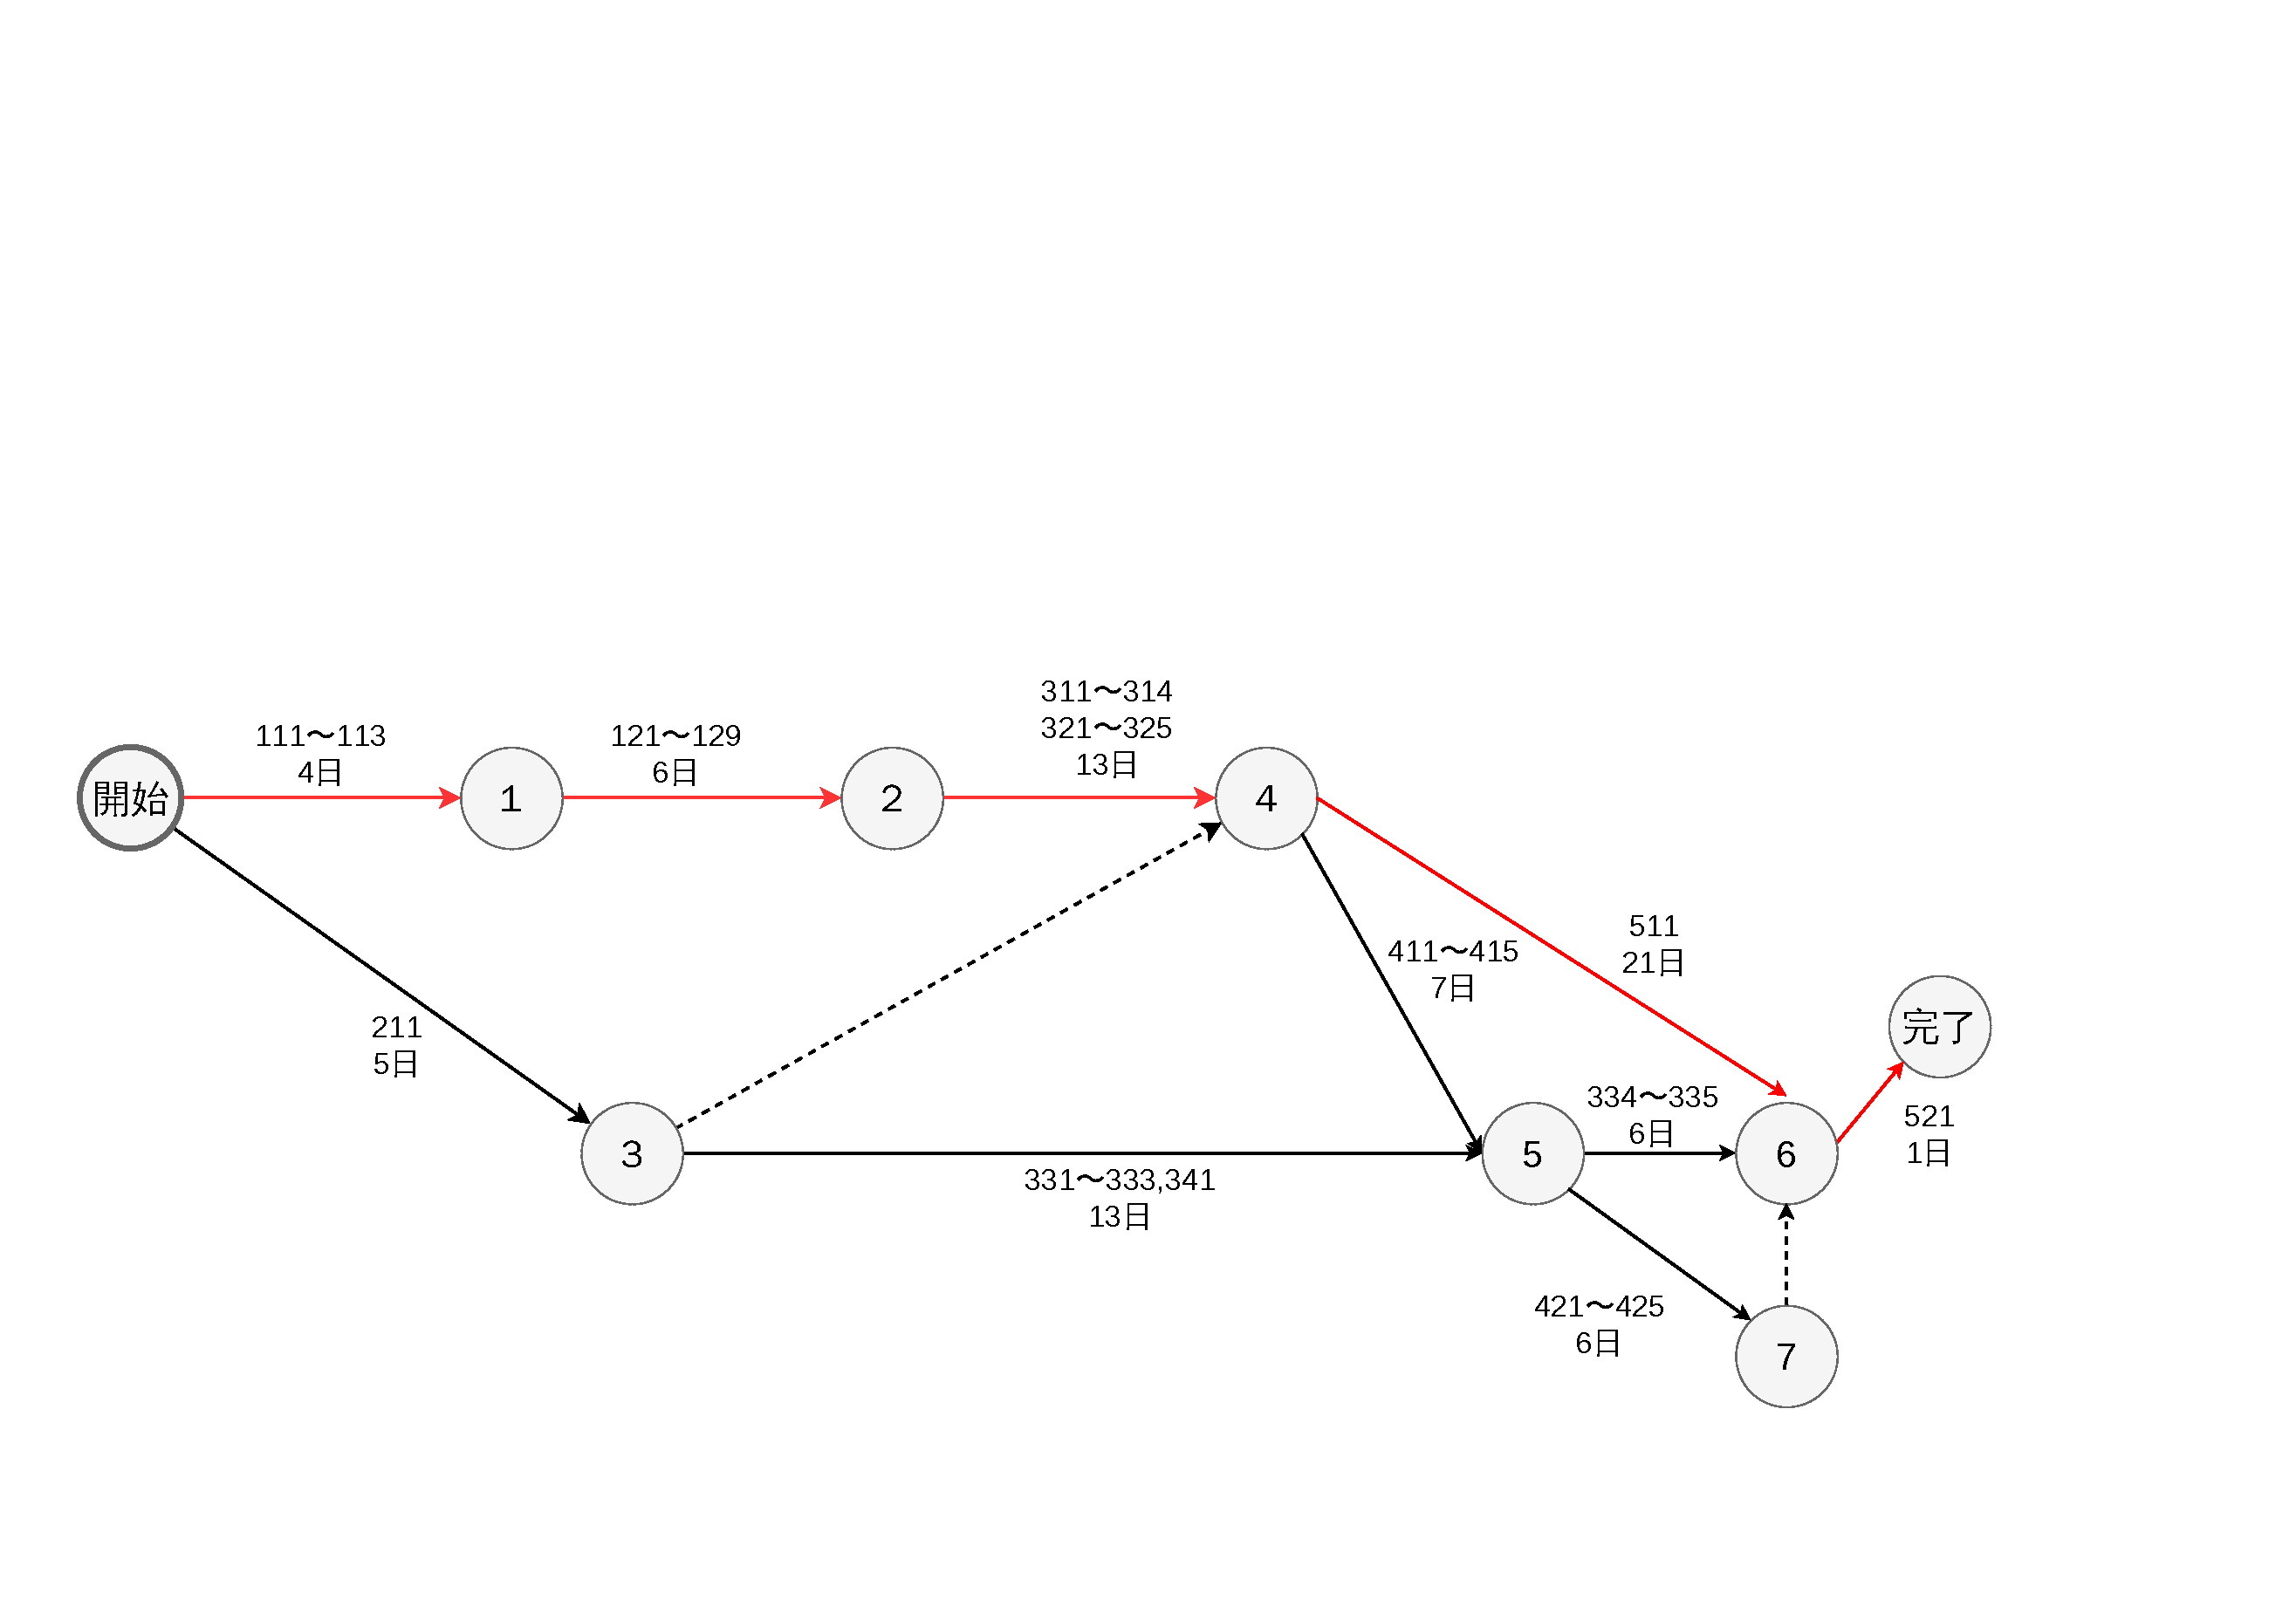
\includegraphics[width=18cm, clip]{img/アローダイアグラム.pdf}
\caption{本開発のアローダイアグラム}
\label{アロー}
\end{center}
\end{figure}
%%%%%%%%%%%%%%%%%%%%%%%%
\subsection{役割分担}
各メンバーの役割分担は表\ref{WBS}に示す通りである．
分担割り当ては，LED点滅機能や受光機能，楽器演奏機能などの本プロジェクトで最低限必要な機能の設計は2年生の飯塚，佐藤，恩田が行う．
また，LEDマトリクス歌詞表示機能やWebサイトでの楽器変更，テンポ変更，音量変更，楽譜選択，ループ演奏選択などの次に必要とする機能の設計を3年生全体で行う．
結合テストおよび機材調達については全員で対応する．
%%%%%%%%%%%%%%%%%%%%%%%%
\subsection{ガントチャート}
本プロジェクトにおけるガントチャートを図\ref{fig:gantt}に示す．
横軸に日付，縦軸にWBSの各タスクを示す．
プロジェクトは2026年5月20日に開始し，設計・機材調達・実装・テストの順に進める．
設計フェーズを5月中に完了させ，6月上旬までに実装，7月頭までにテストを完了することを目標とする．
テスト終了予定日から1週間は，不具合発生時の修正作業および開発遅延への対応を行うための予備期間として確保する．
これにより，リスク管理で想定する遅延や同期精度の問題に対して柔軟に対応できるようにする．
また，中間テストのある6月上旬に，土日を含めた3日間をテスト対策期間として空けている．
\begin{figure}[H]
  \begin{center}
    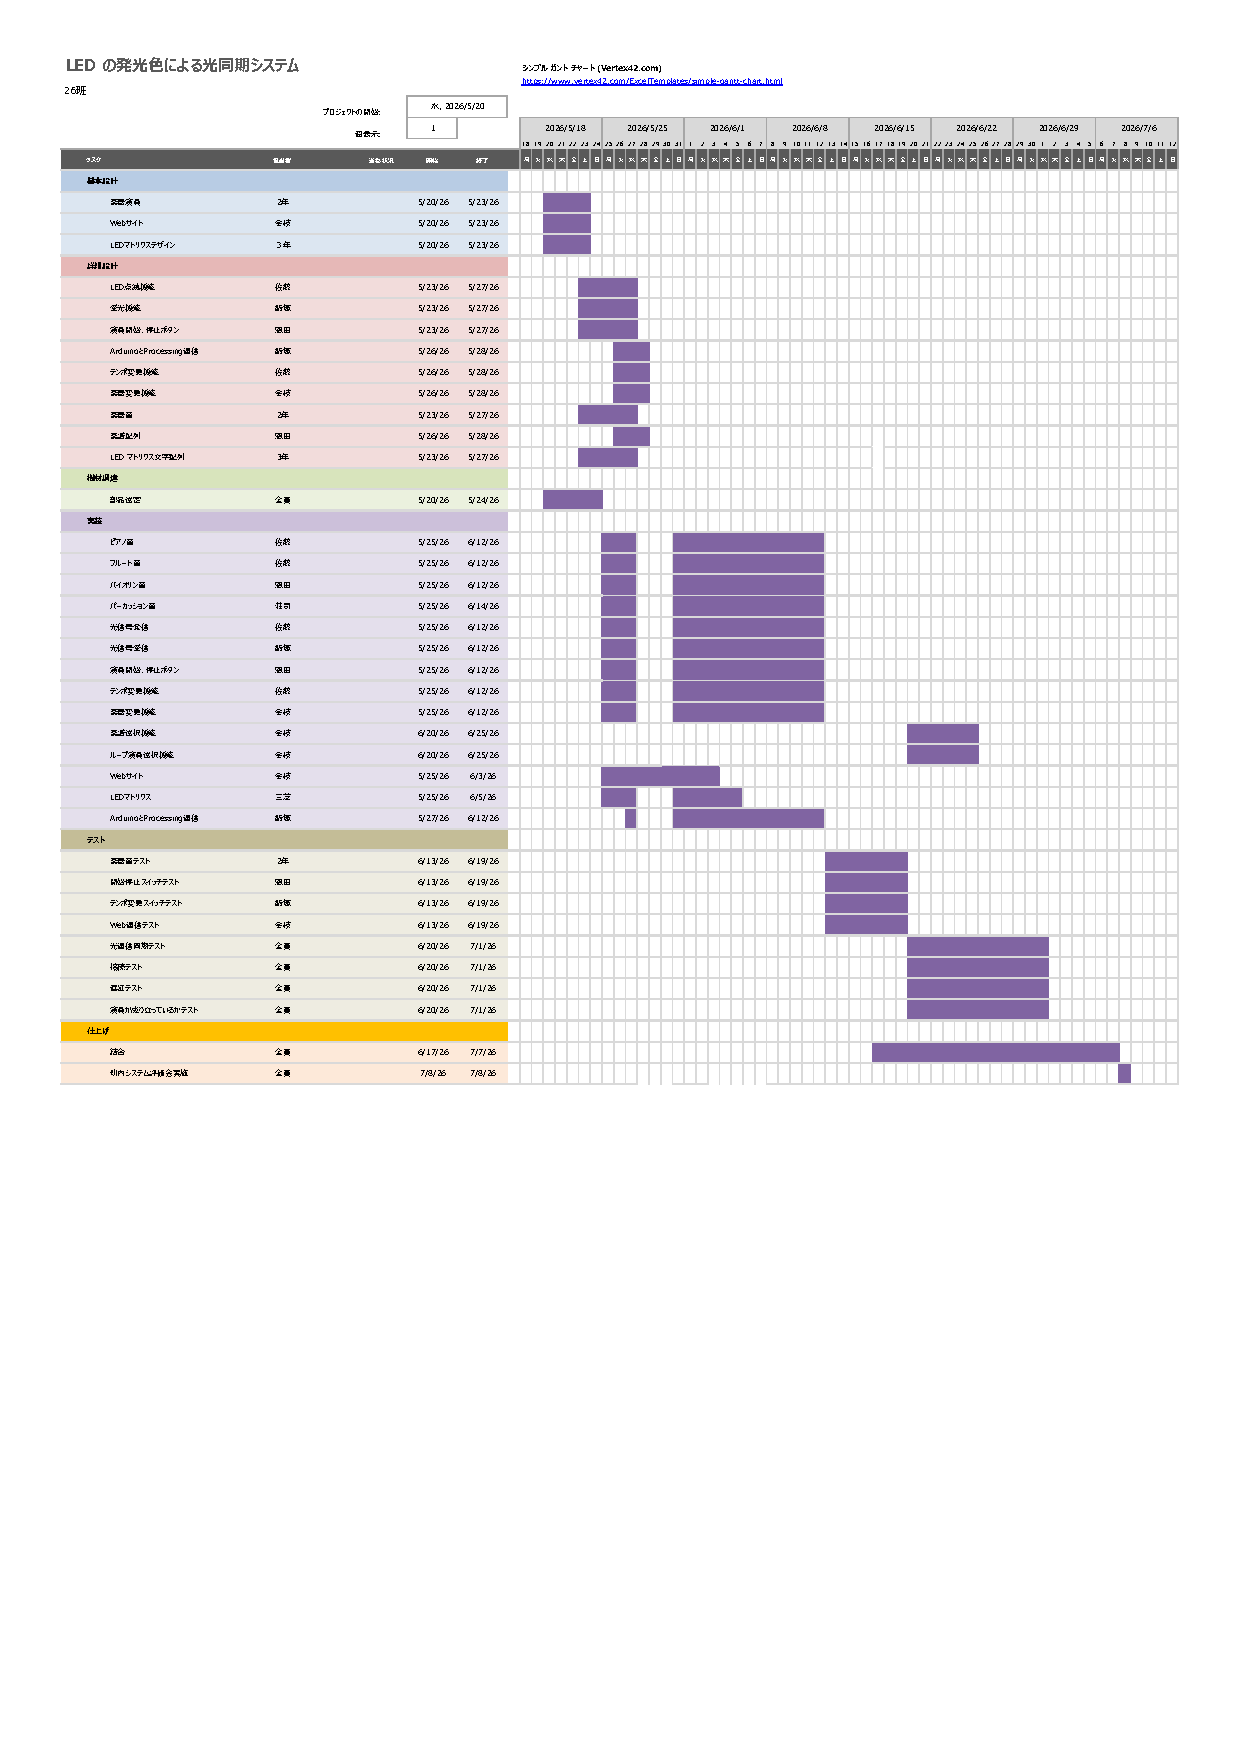
\includegraphics[width=140mm]{./img/gann7_1.pdf}
    \caption[gantt]{ガントチャート}
    \label{fig:gantt}
  \end{center}
\end{figure}
%%%%%%%%%%%%%%%%%%%%%%%%
%%%%%%%%%%%%%%%%%%%%%%%%
\section{検証と妥当性確認: V\&V計画}
%%%%%%%%%%%%%%%%%%%%%%%%
\subsection{プロジェクトの成果物に対する有効指標MOE}
本プロジェクトの成果物は，離れた場所にいる演奏者が指揮者のLEDによる光信号を基準として同期しながら合奏できるシステムである．
このシステムの有効性を評価するための有効指標（MOE）を以下に示す．

\begin{itemize}
    \item \textbf{MOE1：光同期の実現} \\
    指揮者の光信号が各演奏者に遅延なく届き，演奏者間の同期がとれた合奏が成立すること．
    \item \textbf{MOE2：音色の再現性} \\
    本システムが出力する楽器音が，実際の楽器音を十分な精度で再現していること．
    \item \textbf{MOE3：Webサイトによるリアルタイム制御} \\
    指揮者がWebサイトを通じてテンポや楽器などの演奏パラメータをリアルタイムに変更できること．
\end{itemize}
%%%%%%%%%%%%%%%%%%%%%%%%
\subsection{有効指標MOEに対応する性能指標MOP}

各MOEに対応する定量的な性能指標（MOP）を以下に示す．

\begin{table}[h]
\centering
\caption{MOEとMOPの対応}
\begin{tabular}{|c|l|l|r|}
\hline
MOE & 評価項目 & MOP & 目標値 \\
\hline
\multirow{3}{*}{MOE1} & 光と音の発生時間差 & 通信遅延 & 125 ms以内 \\
                       & 演奏者間の同期ズレ & 楽器間同期ズレ & 40 ms以内 \\
                       & 光同期の通信精度   & パケット損失率（IPLR） & 1\%以内 \\
\hline
\multirow{4}{*}{MOE2} & \multirow{4}{*}{楽器音の再現度} & 立ち上がり時間差（AT差） & 60\,ms以内 \\
                       &                                & スペクトル重心相対差（SC差） & 24\%以内 \\
                       &                               & スペクトル変動度差（DSV差） & 16\%以内 \\
                       &                               & 奇偶倍音比差（OER差） & 0.20以内 \\
                       &                               & 音色アンケート評価 & 3.51以上 \\

\hline
\multirow{2}{*}{MOE3} & Webサイトの応答速度 & 送信〜反映までの遅延 & 100 ms以内 \\
                       & Webサイトの通信精度 & パケット損失率（IPLR） & 1\%以内 \\
\hline
\end{tabular}
\end{table}
%%%%%%%%%%%%%%%%%%%%%%%%
\subsection{システムテストで評価する性能指標MOP}
システムテストでは，システム全体を結合した状態で以下のMOPを評価する．

\begin{itemize}
    \item \textbf{光と音の発生時間差（目標：125 ms以内）} \\
    指揮者のLEDが発光してから演奏者PCのスピーカーから音が出るまでの時間差を評価する．
    光（映像）が先，音（音声）が後の場合，125 msを超えるとズレに気づき，185 msを超えると許容できなくなることが知られている\cite{1998}．

    \item \textbf{楽器間の同期ズレ（目標：40 ms以内）} \\
    複数の演奏者間における各拍の発音タイミングのズレを評価する．
    先行音と後続音のズレが40 ms以内であれば一つの音として認識される\cite{brown}．

    \item \textbf{Webサイト送信〜演奏反映までの遅延（目標：100 ms以内）} \\
    WebサイトでテンポなどのパラメータをWebサイトで変更してから，演奏プログラムに反映されるまでの時間を評価する．
    人間がシステムを操作した際，100 ms以内の応答であれば遅延を知覚しない\cite{1968}．
\end{itemize}

%%%%%%%%%%%%%%%%%%%%%%%%
\subsection{結合テストで評価する性能指標MOP}

結合テストでは，各機能モジュールを接続した状態で以下のMOPを評価する．

\begin{itemize}
    \item \textbf{光同期のパケット損失率（目標：1\%以内）} \\
    指揮者から演奏者への光同期通信において，LEDの発光を光センサで検知できたかを計数し，パケット損失率を評価する．
    ITU-Tの規定するリアルタイムデータ通信の許容IPLRは1\%以下である\cite{1541}．

    \item \textbf{Webサイトのパケット損失率（目標：1\%以内）} \\
    Webサイトから演奏プログラムへの制御コマンド送信において，送信ログと受信ログを比較し，パケット損失率を評価する．
    同様にITU-Tの規定する許容IPLRである1\%以下を目標とする\cite{1541}．
\end{itemize}

%%%%%%%%%%%%%%%%%%%%%%%%
\subsection{単体テストで評価する性能指標MOP}

単体テストでは，個々の機能モジュール単体で以下のMOPを評価する．

\begin{itemize}
    \item \textbf{音色の再現性（目標：各音色特徴量が目標差以内）} \\
    実際の楽器音の録音データと，本システムが出力した音の録音データを録音して比較する．

    人間の音色知覚を構成する特徴量である以下の4つを用いて音色の再現精度を評価する\cite{McAdams}．
    比較の前処理として，両者の音量をRMS正規化により統一し，pYINアルゴリズムで推定したF0を用いて音程が一致していることを確認する．
    AT・SC・DSV・OERの4つの音色特徴量を算出し，各音程ごとに参照音源と再現音のズレ量（または相対差）を求め、全音程にわたる平均値を目標値と比較する．
    それぞれの数値の説明は以下に示す．
    本テストは各楽器・音程ごとに行ったうえで平均を取り評価する．

    \textbf{立ち上がり時間（AT）：}RMSエンベロープがピーク値に到達するまでの時間 [ms]．
    音の立ち上がり（アタック）の速さが参照音とどれだけズレているかを評価する．
    音声波形からRMSエンベロープ（短時間ごとのRMS振幅の時系列）を計算し，音が鳴り始めた時点からRMSが最大値（ピーク）に達するまでの時間を求める．
    全音程にわたるズレの平均値を60\,ms以内に収めることを目標とする．
    この数値は，Siedenburg (2019)が10楽器×12音程の実験において，ATを±60ms操作した際の弁別命中率が約79\%になることから決定した\cite{Siedenburg}．
    この水準を「人間が違いに気づきはじめる境界」とみなし，それ未満のズレであれば知覚的に同等とみなせるとし，目標とした．

    \textbf{スペクトル重心（SC）：}持続区間（全体の25〜75\%）でのスペクトル重心周波数 [Hz]．
    音の明るさ・硬さの指標であるスペクトル重心が参照音とどれだけズレているかを評価する．
    音の持続区間（音の長さの25\%〜75\%の区間）についてFFTで周波数スペクトルを求め，各周波数成分をその振幅で重み付けした平均周波数（重心）を計算する．
    SCは$SC = \frac{\sum(f_i \times |X(f_i)|)} { \sum|X(f_i)|}$で求められる．
    ここで$f_i$は周波数、$X(f_i)$は振幅である．
    参照音源と再現音のSC値の相対差（$\frac{|SC_{\mathrm{ref}}-SC_{\mathrm{synth}}|}{SC_{\mathrm{ref}}}\times100$）を音程ごとに算出し，全音程の平均値を求める．
    全音程にわたるSC相対差の平均値を24\%以内に収めることを目標とする．
    この数値はWun et al. (2014)が複数楽器の平均でSCを−24\%変化させると弁別率が75\%を超えることを確認したことに基づき決定した\cite{Wun}．
    この変化量を「聴感上区別がつき始める閾値」とし，それ未満を目標とした．

    \textbf{スペクトル変動度（DSV）：}フレーム間のL2相対変化量の平均 [\%]．
    音の持続中にスペクトル（音色）がどれだけ揺らぐか、その安定性が参照音とどれだけズレているかを評価する．
    音声を短いフレームに分割し，連続するフレーム間でのスペクトル（FFT振幅）の変化量をL2ノルムで算出し，前フレームのスペクトルで正規化した相対変化量を求める．
    参照音源と再現音のDSV値の相対差を音程ごとに算出し，全音程の平均値を求める．
    全音程にわたるDSVズレの平均値を16\%以内に収めることを目標とする．
    この数値はHorner et al. (2004)が8楽器を対象とした実験において，スペクトル変動誤差が16\%程度で知覚上の弁別が中程度となることを報告していることに基づき決定した\cite{Horner}．
    これを許容できる誤差の上限として採用した．

    \textbf{奇偶倍音比（OER）：}奇偶倍音比
    奇数倍音と偶数倍音のバランス（楽器固有の音色を決定づける要素．例：クラリネットは奇数倍音優位，フルートは均等）が参照音とどれだけズレているかを評価する．
    pYINアルゴリズム\cite{pyin}でF0（基本周波数）を推定し，n$\times$F0 （n=1,2,3…）の位置にある倍音成分のエネルギーを抽出する．
    奇数次倍音のエネルギー合計をE\_odd、偶数次倍音のエネルギー合計をE\_evenとし，$E_{\mathrm{odd}}/(E_{\mathrm{odd}}+E_{\mathrm{even}})$を算出する．
    参照音源と再現音のOER値の相対差を音程ごとに算出し，全音程の平均値を求める．
    全音程にわたるOER相対差の平均値を20\%以内に収めることを目標とする．
    Caclin et al. (2005)がスペクトル不規則性（奇偶倍音比はその指標の一つ）が音色知覚の重要な相関物であることを実験的に確認した\cite{Caclin}こと，
    McAdams et al. (1995)の知覚次元モデルとも一致するため，相対差20\%以内を目標とした\cite{McAdams}．


\end{itemize}

音色の知覚には倍音構成・エンベロープ・ノイズ成分など無数の物理的特徴が関わるが，心理学的な多次元尺度構成法（MDS）を用いた聴取実験から，人間が実際に音色を判断する際に利用している主要な次元はごく少数に絞り込めることが示されている．
McAdams et al. (1995)は楽器音に対する非類似度判断をMDS分析し，人間の音色知覚が「立ち上がり時間（時間的特徴）」「スペクトル重心（明るさ）」「スペクトル変動度（音色の時間的揺らぎ）」というごく少数の次元でほぼ説明できることを示した\cite{McAdams}．
AT・SC・DSVはこの主要3次元に直接対応する指標である．
一方，この3次元だけでは一部の楽器に残る差（楽器固有の「特異性」）を説明できないことも示されており,Caclin et al. (2005)はその主な要因がスペクトル不規則性（奇数次倍音と偶数次倍音のエネルギーバランスの偏り）であることを実験的に確認した\cite{Caclin}．
OERはこの第4の次元に対応する指標である．
つまりAT・SC・DSVが音色知覚の主要3次元，OERがそれだけでは捉えきれない楽器固有の特異性を補う指標として機能しており，この4つを組み合わせることで人間が実際に音色の違いとして知覚する範囲をほぼ網羅的に説明できる．
そのため，4項目すべてが目標差以内に収まっていれば，人間が知覚する音色差は小さいと考えられ，参照音源と再現音は知覚上おおむね類似した音色を有すると判断できる．

また，音色の評価に関して，AT・SC・DSV・OERの4つの音色特徴量の算出の他にアンケートも同時に行う．
作成した回答用フォームを用いた音色評価を実施し，その結果を元に評価を行う．
この音色評価は，参加者に作成した音と実際の楽器の音を聞き比べてもらい，目的音をどの程度再現できているかを以下の5段階で評価してもらい，その平均値を用いて評価する．
集計したものの平均が3.51以上の場合，音色が十分再現されていると判断する．
音色の評価では，AT・SC・DSV・OERによる音響特徴量の解析結果と，アンケートによる聴取評価の双方を用いて総合的に評価する．


%%%%%%%%%%%%%%%%%%%%%%%%
\subsection{プロジェクト中に監視する技術性能指標TPM}
作業分解構造に基づくタスクの消化進捗率を監視する．
当初の予定に対して進捗の遅延が15％を超えた場合には，楽器変更機能などの付加的な機能の優先順位を下げ，コアとなる合奏同期機能の完成を最優先する．

プロジェクト実行中に監視する技術性能指標TPMを表\ref{TPM}に示す．
演奏同期は，光信号受信から演奏開始までの遅延を測定し，100msを超えた場合には通信方式や処理手順を見直す．
楽器演奏は，出力音の周波数を測定し，基準周波数との差を確認する．
誤差が大きい場合には，発振周波数や音源生成処理を調整する．
LEDマトリクス歌詞表示は，演奏タイミングとのズレを測定し，±100msを超える場合には表示更新処理の改善を行う．

これらのTPMを継続的に監視することで，
システム全体の品質向上と問題の早期発見を目指す
\begin{table}[H]
\centering
\caption{技術性能指標TPM}
\label{TPM}
\resizebox{\textwidth}{!}{
\begin{tabular}{|l|l|l|} \hline
FBS要素 & 監視指標 & 理由 \\ \hline
演奏同期 & 光信号受信から演奏開始までの遅延 & 同期はシステムの根幹にかかわるため \\ \hline
楽器演奏 & 参考周波数とのズレ & 音程の正確さはシステムの品質に直結するため \\ \hline
LEDマトリクス歌詞表示 & 演奏タイミングと歌詞表示のズレ & 視覚情報の同期はシステムの完成度にかかわるため \\ \hline
\end{tabular}
}
\end{table}


%%%%%%%%%%%%%%%%%%%%%%%%
%%%%%%%%%%%%%%%%%%%%%%%%
\section{資源・調達管理}
本開発にあたって必要な機材とその調達方法を表\ref{使用機材}に示す．
\begin{table}
 \begin{center}
   \caption{使用機材一覧}
   \label{使用機材}
  \begin{tabular}{|l|l|l|l|l|}
	\hline
    使用機材&型番& 単価(円) & 個数 &調達方法\\\hline
    マイコンボード&Arduino UNO R4 WiFi& 0 & 5 &所有 \\\hline
	  抵抗器330 $\Omega$&-& 6 & - &所有 \\\hline
    抵抗器3300 $\Omega$&-& 1 & - &所有 \\\hline
	  ブレッドボード & 165401020E & 0 & 3 & 所有 \\\hline
    ジャンパワイヤー & 165012000E & 0 & 1式 & 所有 \\\hline
	  カラーセンサ&TCS34725&500&4&Amazonにて購入\\\hline
	  カラーLED&OSTA5131A-R/PG/B& 50 &2&秋月電子通商にて購入\\\hline
	  Processing実行用PC&MacBook Air/Pro& - & 5台 & 所有\\\hline
	  USB Type-C to Cケーブル & - & - &  5 & 所有\\\hline
    タクトスイッチ & - & - &  1 & 学科借用\\\hline
    可変抵抗器 & RK09D117000B & 60 &  1 & 秋月電子通商にて購入\\\hline
    ルータ & - & 0 &  1 & 学科借用\\\hline
    覆いの箱 & - & 0 & 1 & 班員私物\\\hline
  \end{tabular}
 \end{center}
\end{table}

\clearpage
%%%%%%%%%%%%%%%%%%%%%%%%
%%%%%%%%%%%%%%%%%%%%%%%%
\section{リスク管理}
本プロジェクトにおいて，光同期の精度が低い，進捗が遅く実装が間に合わないなどのリスクが考えられる．
光同期の精度が低い場合，周囲の光によるノイズなどの外部からのノイズを排除するために，光通信全体を仕切りで覆うなどの処置を施す．
進捗が遅く実装が間に合わない場合，進捗が十分なメンバーが終わっていない作業のサポートを行い，それでも間に合わない場合は優先順位の低い追加機能の実装を諦めることとする．
これらをまとめた，リスク内容と発生可能性並びに影響度，対策を表\ref{リスク管理}に示す．

\begin{table}
 \begin{center}
   \caption{リスク管理}
   \label{リスク管理}
   \resizebox{\textwidth}{!}{ 
  \begin{tabular}{|l|l|l|l|}
	\hline
    リスク内容&発生可能性& 影響 & 対策\\\hline
	光通信の精度が出ない&高&大&センサの感度調整・遮光対策を行う\\\hline
	遅延が大きく同期がとれない&中&大&テストを早めに行い早期発見する\\\hline
	想定より実装に時間がかかる&中&大&クリティカルパスを優先し，余裕日数を活用する\\\hline
	メンバー間で進捗に差が出る&中&中&進捗をこまめに共有し，タスクを再分配する\\\hline
	データの紛失&低&大&GitHubなどでバージョン管理を行う\\\hline
	部品が届かない・壊れる&低&中&予備部品を確保しておく\\\hline
  \end{tabular}
   }
 \end{center}
\end{table}


%%%%%%%%%%%%%%%%%%%%%%%%
%%%%%%%%%%%%%%%%%%%%%%%%
%%%%%%%%%%%%%%%%%%%%%%%%
\chapter{システムの基本設計}
% 設計書は作成する成果物によって変化します．
% 適宜修正して利用してください．


%%%%%%%%%%%%%%%%%%%%%%%%
\section{機能一覧}
% 機能分解構造FBSの要素の説明
本システムの機能一覧をFBSに基づいて表\ref{機能一覧}に示す．
本システムは，指揮者と複数の演奏者からなるオーケストラ形式の同期演奏を実現するための多様な機能を備えている．
システムの根幹となる制御機能は，指揮者用Arduinoに直接取り付けられたスイッチによって管理され，これによりLEDの点滅開始と終了，すなわち演奏の開始と停止を即座に行うことが可能である．
通信においては，フルカラーLEDを用いた独自の光通信プロトコルを採用しており，発光色によって各Arduinoの演奏開始を指示する．
なお，再生する楽器音はWebサイトから事前に指定された楽器IDに従うため，色と楽器音は直接対応しない．
点滅間隔の長さによって楽曲のテンポを精密に調整する．
また，LEDの点滅の強さ，すなわち光量のピーク値を算出することで，各楽器の音量を動的に変化させることができ，柔軟な強弱表現を可能としている．

ユーザーとのインターフェースとして機能するWebサイトからは，テンポ変更や全体音量の調節，演奏者ごとの個別音量の調節に加えて，演奏の開始と停止，楽譜選択，ループ演奏選択といった高度な演奏制御が行える．さらに，ネットワーク環境に問題が発生するなどしてWebサイトが利用できない事態を想定し，可変抵抗によるアナログ電圧変化を用いたテンポ調整機能もあわせて実装する．
視覚的な演出面では，演奏者側のArduinoに搭載されたLEDマトリクスのうち，横8$\times$縦8の範囲を利用して歌詞を一文字ずつ表示する．
楽譜情報の送信進捗に合わせた動的なテキスト表示をすることによって，エンターテインメント性における独創性を高めている．
% 本システムが備える主要な機能を以下の表にまとめる．
\begin{table}[H]
\centering
\caption{本システムの機能一覧}
\label{機能一覧}
\begin{tabular}{|p{3.5cm}|p{9.5cm}|}
\hline
\textbf{機能名} & \textbf{機能概要} \\ \hline
システム起動・停止 & 指揮者用Arduinoに取り付けられた物理スイッチを操作することで，全体の演奏開始および終了を制御する． \\ \hline
光信号同期通信 & 指揮者側LEDの発光色によって各パートの演奏開始を指示し，点滅間隔の長さに基いてテンポを調節する． \\ \hline
Web遠隔制御 & Webブラウザを介して，BPMの指定，全体音量の調節，楽器パートの変更，楽譜選択，演奏者ごとの個別音量の調節，およびループ演奏の切り替えを指示する． \\ \hline
楽器音合成・再生 & 演奏者側PCのProcessing上で，受信した音高，光量由来の音強，点滅由来の音長情報を基に波形を合成し再生する． \\ \hline
個別音量・表現制御 & LEDの点滅の強さ（光量のピーク値）から個別の音量倍率を算出し，動的な音楽表現を実現する． \\ \hline
歌詞表示演出 & LEDマトリクスの横8$\times$縦8範囲を利用し，カタカナを用いて歌詞を一文字ずつ表示する．輪唱において各パートが異なるタイミングで演奏を開始するため，聴覚のみでは把握しにくい演奏構造を視覚情報として補完する． \\ \hline
アナログ制御（予備） & ネットワーク環境等によりWeb制御が困難な場合，可変抵抗の電圧変化を利用してテンポを可変させる． \\ \hline
同期確認用LED（箱外） & 視覚フィードバックおよび遅延計測用に使用するLED，指揮者側LEDと同じ光り方をする． \\ \hline
\end{tabular}
\end{table}

%%%%%%%%%%%%%%%%%%%%%%%%
\section{システム構成図}
% ハードウェア，ソフトウェアなどの構成図を記載する．
ここで，システム全体の構成図を図\ref{fig:system_config}に示す．
\begin{figure}[H]
  \centering
  % 図全体を紙面幅に自動調整し，はみ出しを防止します
  \resizebox{\textwidth}{!}{
    \begin{tikzpicture}[
      auto,
      % ブロックの基本スタイル設定
      block/.style={rectangle, draw, thick, text width=3cm, align=center, minimum height=1.3cm},
      % 矢印のスタイル設定
      line/.style={draw, thick, -{Stealth[length=2.5mm]}},
      font=\small,
      % ノード間の距離（縦 2cm, 横 4.5cm）
      node distance=2cm and 4.5cm
    ]

    % --- 中央：中核となるArduino ---
    \node [block] (conductor) {指揮者Arduino};
    \node [block, right=6cm of conductor] (player) {演奏者Arduino \\ (光センサ)};
    \node [below=0.3cm of player, text width=5cm, align=center, font=\footnotesize] {＊外来光を防ぐ覆いを設置};

    % --- 左側：指揮者への入力 ---
    \node [block, left=5cm of conductor] (switch) {物理スイッチ};
    \node [block, above=1.5cm of switch] (web) {PC \\ (Webブラウザ)};
    \node [block, below=1.5cm of switch] (resistor) {可変抵抗};

    % --- 右側：演奏者からの出力 ---
    \node [block, right=4cm of player, yshift=1.5cm] (processing) {PC \\ (Processing)};
    \node [block, right=4cm of player, yshift=-1.5cm] (matrix) {LEDマトリクス};
    \node [block, right=2.5cm of processing] (speaker) {スピーカー};

    % --- 矢印とラベルの描画 ---
    % 指揮者側：重複を避けるためラベルを改行
    \draw [line] (web.east) -- ++(1,0) |- node[pos=0.4, right, font=\footnotesize, align=left] {起動・停止信号，\\BPM，全体音量，ループ} (conductor.160);
    \draw [line] (switch.east) -- node[above, font=\footnotesize] {起動・停止信号} (conductor.180);
    \draw [line] (resistor.east) -- ++(1,0) |- node[pos=0.4, right, font=\footnotesize] {アナログ電圧(BPM)} (conductor.200);
    \draw [line] (web.north) -- ++(0, 0.8) -| node[pos=0.25, above, font=\footnotesize, align=center] {楽器指定，楽譜選択，個別音量} (player.north);

    % 中央：光信号
    \draw [line] (conductor) -- node[above, align=center, font=\footnotesize] {光信号(LED点滅)} 
                                 node[below, align=center, font=\footnotesize] {発光色(開始)，点滅間隔(テンポ)\\光量ピーク(音量)} (player);

    % 演奏者側
    \draw [line] (player.east) -- ++(0.8,0) |- node[pos=0.75, above, font=\footnotesize, align=center] {音高，音量倍率，\\音長データ，楽器ID} (processing.west);
    \draw [line] (player.east) -- ++(0.8,0) |- node[pos=0.4, right, font=\footnotesize] {歌詞表示データ} (matrix.west);
    \draw [line] (processing) -- node[above, font=\footnotesize] {音の再生} (speaker);

    \end{tikzpicture}
  }
  \caption{システム構成図}
  \label{fig:system_config}
\end{figure}

%%%%%%%%%%%%%%%%%%%%%%%%
\section{操作インターフェース設計}
% 画面やスイッチなどのインターフェースの設計図を記載する
本システムの操作インターフェースでは，主系統であるWebブラウザUIと，予備系統である物理的なアナログ入力の両方を設計する．

主系統のインターフェースとして，WiFiネットワーク経由のHTTP通信を利用したブラウザベースのコントロールパネルを用意する．
図\ref{fig:web_ui}にWebブラウザのUI配置を示す．
\begin{figure}[H]
  \centering
  \begin{tikzpicture}[
    auto,
    element/.style={draw, thick, rectangle, rounded corners=3pt, minimum height=0.55cm, align=center},
    panel/.style={draw, thick, rectangle, rounded corners=6pt, fill=gray!5},
    card/.style={draw, thick, rectangle, rounded corners=5pt, fill=white, minimum width=5.8cm, minimum height=4.2cm},
    btn/.style={draw, thick, rectangle, rounded corners=3pt, minimum height=0.55cm, align=center}
  ]

  % 全体背景パネル
  \node[panel, minimum width=17cm, minimum height=18cm] (bg) at (0, 0) {};

  % タイトル・サーバーIP
  \node[font=\large\bfseries] at (0, 8.3) {Arduino オーケストラ コントロールパネル};
  \node[font=\small, text=green!60!black] at (0, 7.5) {サーバーIP: 192.168.xx.xx};

  % ── 指揮者セクション ──
  \node[panel, minimum width=15.5cm, minimum height=4.6cm] at (0, 5.5) {};
  \node[right, font=\small\bfseries] at (-7.3, 7.0) {【指揮者】};

  % BPM
  \node[right, font=\small] at (-7.0, 6.3) {BPM:};
  \draw[thick] (-5.0, 6.3) -- (3.5, 6.3);
  \filldraw[fill=blue!60, draw=blue!60] (0.5, 6.3) circle (0.15cm);
  \node[font=\small] at (4.2, 6.3) {120};
  \node[btn, fill=blue!15, minimum width=1.0cm, font=\small] at (5.8, 6.3) {送信};

  % 全体音量
  \node[right, font=\small] at (-7.0, 5.5) {全体音量:};
  \draw[thick] (-5.0, 5.5) -- (5.5, 5.5);
  \filldraw[fill=blue!60, draw=blue!60] (5.2, 5.5) circle (0.12cm);
  \node[font=\small] at (6.0, 5.5) {MAX};

  % 演奏ボタン
  \node[right, font=\small] at (-7.0, 4.7) {演奏:};
  \node[btn, fill=green!25, minimum width=4.0cm, font=\small] at (-2.0, 4.7) {開始};
  \node[btn, fill=red!25, minimum width=4.0cm, font=\small] at (3.8, 4.7) {停止};

  % ループ（トグルスイッチ）
  \node[right, font=\small] at (-7.0, 3.9) {ループ:};
  \draw[thick, rounded corners=6pt, fill=gray!25] (-5.0, 3.6) rectangle (-3.4, 4.2);
  \filldraw[fill=white, draw=gray!70, thick] (-4.75, 3.9) circle (0.28cm);
  \node[font=\small] at (-2.9, 3.9) {OFF};

  % ── 演奏者セクション ──
  \node[right, font=\small\bfseries] at (-7.3, 2.8) {【演奏者】};

  % 演奏者1（左上）
  \node[card, minimum width=7.2cm, minimum height=4.8cm] at (-3.8, 0.2) {};
  \node[right, font=\small\bfseries] at (-7.1, 2.0) {演奏者 1};
  \node[right, font=\small] at (-7.1, 1.1) {楽器:};
  \node[element, fill=white, minimum width=3.2cm, font=\small] at (-3.2, 1.1) {ピアノ $\nabla$};
  \node[right, font=\small] at (-7.1, 0.1) {個別音量:};
  \draw[thick] (-5.0, 0.1) -- (-1.2, 0.1);
  \filldraw[fill=blue!60, draw=blue!60] (-1.5, 0.1) circle (0.10cm);
  \node[font=\footnotesize] at (-0.6, 0.1) {MAX};
  \node[right, font=\small] at (-7.1, -0.9) {楽譜:};
  \node[element, fill=white, minimum width=3.2cm, font=\small] at (-3.2, -0.9) {リズム $\nabla$};
  \node[btn, fill=blue!15, minimum width=1.0cm, font=\small] at (-0.8, -1.8) {送信};

  % 演奏者2（右上）
  \node[card, minimum width=7.2cm, minimum height=4.8cm] at (3.8, 0.2) {};
  \node[right, font=\small\bfseries] at (0.3, 2.0) {演奏者 2};
  \node[right, font=\small] at (0.3, 1.1) {楽器:};
  \node[element, fill=white, minimum width=3.2cm, font=\small] at (4.4, 1.1) {ピアノ $\nabla$};
  \node[right, font=\small] at (0.3, 0.1) {個別音量:};
  \draw[thick] (1.8, 0.1) -- (6.5, 0.1);
  \filldraw[fill=blue!60, draw=blue!60] (6.2, 0.1) circle (0.10cm);
  \node[font=\footnotesize] at (7.0, 0.1) {MAX};
  \node[right, font=\small] at (0.3, -0.9) {楽譜:};
  \node[element, fill=white, minimum width=3.2cm, font=\small] at (4.4, -0.9) {リズム $\nabla$};
  \node[btn, fill=blue!15, minimum width=1.0cm, font=\small] at (6.8, -1.8) {送信};

  % 演奏者3（左下）
  \node[card, minimum width=7.2cm, minimum height=4.8cm] at (-3.8, -4.5) {};
  \node[right, font=\small\bfseries] at (-7.1, -2.7) {演奏者 3};
  \node[right, font=\small] at (-7.1, -3.6) {楽器:};
  \node[element, fill=white, minimum width=3.2cm, font=\small] at (-3.2, -3.6) {ピアノ $\nabla$};
  \node[right, font=\small] at (-7.1, -4.6) {個別音量:};
  \draw[thick] (-5.0, -4.6) -- (-1.2, -4.6);
  \filldraw[fill=blue!60, draw=blue!60] (-1.5, -4.6) circle (0.10cm);
  \node[font=\footnotesize] at (-0.6, -4.6) {MAX};
  \node[right, font=\small] at (-7.1, -5.6) {楽譜:};
  \node[element, fill=white, minimum width=3.2cm, font=\small] at (-3.2, -5.6) {リズム $\nabla$};
  \node[btn, fill=blue!15, minimum width=1.0cm, font=\small] at (-0.8, -6.5) {送信};

  % 演奏者4（右下）
  \node[card, minimum width=7.2cm, minimum height=4.8cm] at (3.8, -4.5) {};
  \node[right, font=\small\bfseries] at (0.3, -2.7) {演奏者 4};
  \node[right, font=\small] at (0.3, -3.6) {楽器:};
  \node[element, fill=white, minimum width=3.2cm, font=\small] at (4.4, -3.6) {ピアノ $\nabla$};
  \node[right, font=\small] at (0.3, -4.6) {個別音量:};
  \draw[thick] (1.8, -4.6) -- (6.5, -4.6);
  \filldraw[fill=blue!60, draw=blue!60] (6.2, -4.6) circle (0.10cm);
  \node[font=\footnotesize] at (7.0, -4.6) {MAX};
  \node[right, font=\small] at (0.3, -5.6) {楽譜:};
  \node[element, fill=white, minimum width=3.2cm, font=\small] at (4.4, -5.6) {リズム $\nabla$};
  \node[btn, fill=blue!15, minimum width=1.0cm, font=\small] at (6.8, -6.5) {送信};

  % 全演奏者に一括送信
  \node[btn, fill=cyan!20, minimum width=15cm, minimum height=0.9cm, font=\small] at (0, -7.7) {全演奏者に一括送信};

  \end{tikzpicture}
  \caption{WebブラウザのUI配置}
  \label{fig:web_ui}
\end{figure}

システムを運用するための各種入力フォームが直感的に操作できるよう配置する．
具体的には，楽曲のテンポを数値で指定するBPM入力欄，全体音量を調節するスライダー，演奏の開始・停止ボタン，ループ演奏のトグルスイッチを指揮者セクションに配置する．
また，演奏者ごとに楽器の変更，個別音量の調節，楽譜の選択が行える演奏者カードを設ける．
入力された各種パラメータは，送信ボタンを押すことでHTTP通信によってArduinoへ送信される仕組みである．


一方，予備系統のインターフェースとして，ネットワーク障害やPCの不具合等によりWeb UIが利用不可能な事態を想定し，
指揮者用Arduinoに直接接続された可変抵抗を用いた物理的な操作機構を用意する．
可変抵抗を操作することによって生じるアナログ電圧の変化をArduinoのA/Dコンバータで読み取り，
その数値をBPMにマッピングすることで，直感的なテンポ制御を可能とする．これにより，
不測の事態においても合奏の続行は担保することができる設計となっている．

%%%%%%%%%%%%%%%%%%%%%%%%
\section{状態遷移図}
本システムの中心となる指揮者用Arduinoは，外部からの入力に応じて複数の状態を遷移しながら動作を継続する．図\ref{fig:state_transition}にその詳細な状態遷移を示す．
システムの電源投入および初期設定の完了後，デバイスは「待機・定周期点滅状態」へと移行し，接続要求を待つ．
この状態においてWebブラウザからBPM情報を受信した場合「BPM更新処理」へと遷移し，内部変数の書き換えが完了した後に
再び待機状態へと復帰する．

また，指揮者用Arduinoに搭載された物理スイッチが押下（ON）されると，システムは「演奏・同期信号送出状態」へと移行し，
設定されたBPMに基づいた光信号の送出を開始する．演奏中に再度スイッチが押下（OFF）される，あるいはWebブラウザから
停止命令を受信した場合には，信号送出を停止して初期の待機状態へと遷移する仕組みである．
\begin{figure}[H]
  \centering
  \begin{tikzpicture}[
    auto,
    node distance=3.5cm and 5.5cm,
    state/.style={circle, draw, thick, minimum size=3.2cm, align=center, font=\small},
    arrow/.style={-Stealth, thick, font=\footnotesize}
  ]

  % 状態ノードの配置
  \node[state] (standby) {待機・\\定周期点滅};
  \node[state, above=of standby] (update) {BPM\\更新処理};
  \node[state, right=of standby] (play) {演奏・\\同期信号送出};

  % 開始矢印
  \draw[arrow] (standby.west) ++(-1.5,0) -- node[above] {電源投入} (standby.west);

  % 遷移矢印
  \draw[arrow] (standby.110) -- node[left] {WebよりBPM受信} (update.250);
  \draw[arrow] (update.290) -- node[right] {更新完了} (standby.70);

  \draw[arrow] (standby.20) -- node[above, align=center] {スイッチ押下\\(ON)} (play.160);
  \draw[arrow] (play.200) -- node[below, align=center] {スイッチ押下(OFF)\\または停止命令受信} (standby.340);

  \end{tikzpicture}
  \caption{指揮者Arduinoの状態遷移図}
  \label{fig:state_transition}
\end{figure}

%%%%%%%%%%%%%%%%%%%%%%%%
%%%%%%%%%%%%%%%%%%%%%%%%
%%%%%%%%%%%%%%%%%%%%%%%%
\chapter{システムの詳細設計}

% 設計書は作成する成果物によって変化します．
% 適宜修正して利用してください．


%%%%%%%%%%%%%%%%%%%%%%%%
\section{部品一覧}
% 製品分解構造PBSの要素の説明
本システムを構築するために使用する主要なハードウェア部品の一覧を表\ref{tab:parts_list}に示す．

\begin{table}[H]
\centering
\caption{本システムの主要部品一覧}
\label{tab:parts_list}
\begin{tabular}{|p{3.5cm}|p{2.5cm}|p{8.5cm}|}
\hline
\textbf{部品名} & \textbf{型番・仕様} & \textbf{用途および選定理由} \\ \hline
マイクロコントローラ & Arduino Uno R4 WiFi & 指揮者側および演奏者側のメイン制御を行う．PCとのシリアル通信や，センサ・LEDの高速な制御に必要な処理能力を満たす． \\ \hline
カラーセンサ & TCS34725 & 演奏者側デバイスにおいて，指揮者側からの光信号（発光色および光量）を読み取るために使用する．RGB値に加えてClear値（光量そのものの値）を直接出力できる特性を持つため，音量計算用の値を直接測定することができ，処理負荷の軽減が期待できる点が選定の決め手となった． \\ \hline
フルカラーLED & OSTA5131A-R/PG/B & 指揮者側デバイスにおいて，演奏開始・停止，テンポ，および音量の各情報を，発光色，点滅間隔，光強度という光信号に変換して空間へ送出するために使用する． \\ \hline
LEDマトリクス & 8$\times$8 ドット & 演奏者側デバイスにおいて，楽曲の進行に合わせて歌詞を表示する演出用ディスプレイとして使用する．解像度の制約上，カタカナを一文字ずつ描画する．Arduino Uno R4 WiFi内蔵のものを利用する． \\ \hline
物理スイッチ & タクトスイッチ & 指揮者側デバイスにおいて，システム全体の合奏を物理的に起動および停止させるためのトリガー入力として使用する． \\ \hline
可変抵抗 & ポテンショメータ & Webインターフェースがネットワーク障害等で使用できない場合の予備系統として用意する．ツマミの回転によるアナログ電圧変化をBPM制御に利用する． \\ \hline
\end{tabular}
\end{table}
%%%%%%%%%%%%%%%%%%%%%%%%
%%%%%%%%%%%%%%%%%%%%%%%%
\section{ハードウェア設計}
本システムのハードウェアは，図\ref{fig:system_overview}に示すように，独立した指揮者デバイスと演奏者デバイスの2種類の筐体で構成される．
本ハードウェア構成にした理由は，指揮者の出すLED同期信号を複数の演奏者が同時に受信し遅延を減少させることを目的としたため，図\ref{fig:system_overview}のように構成した．
\begin{figure}[H]
  \begin{center}
    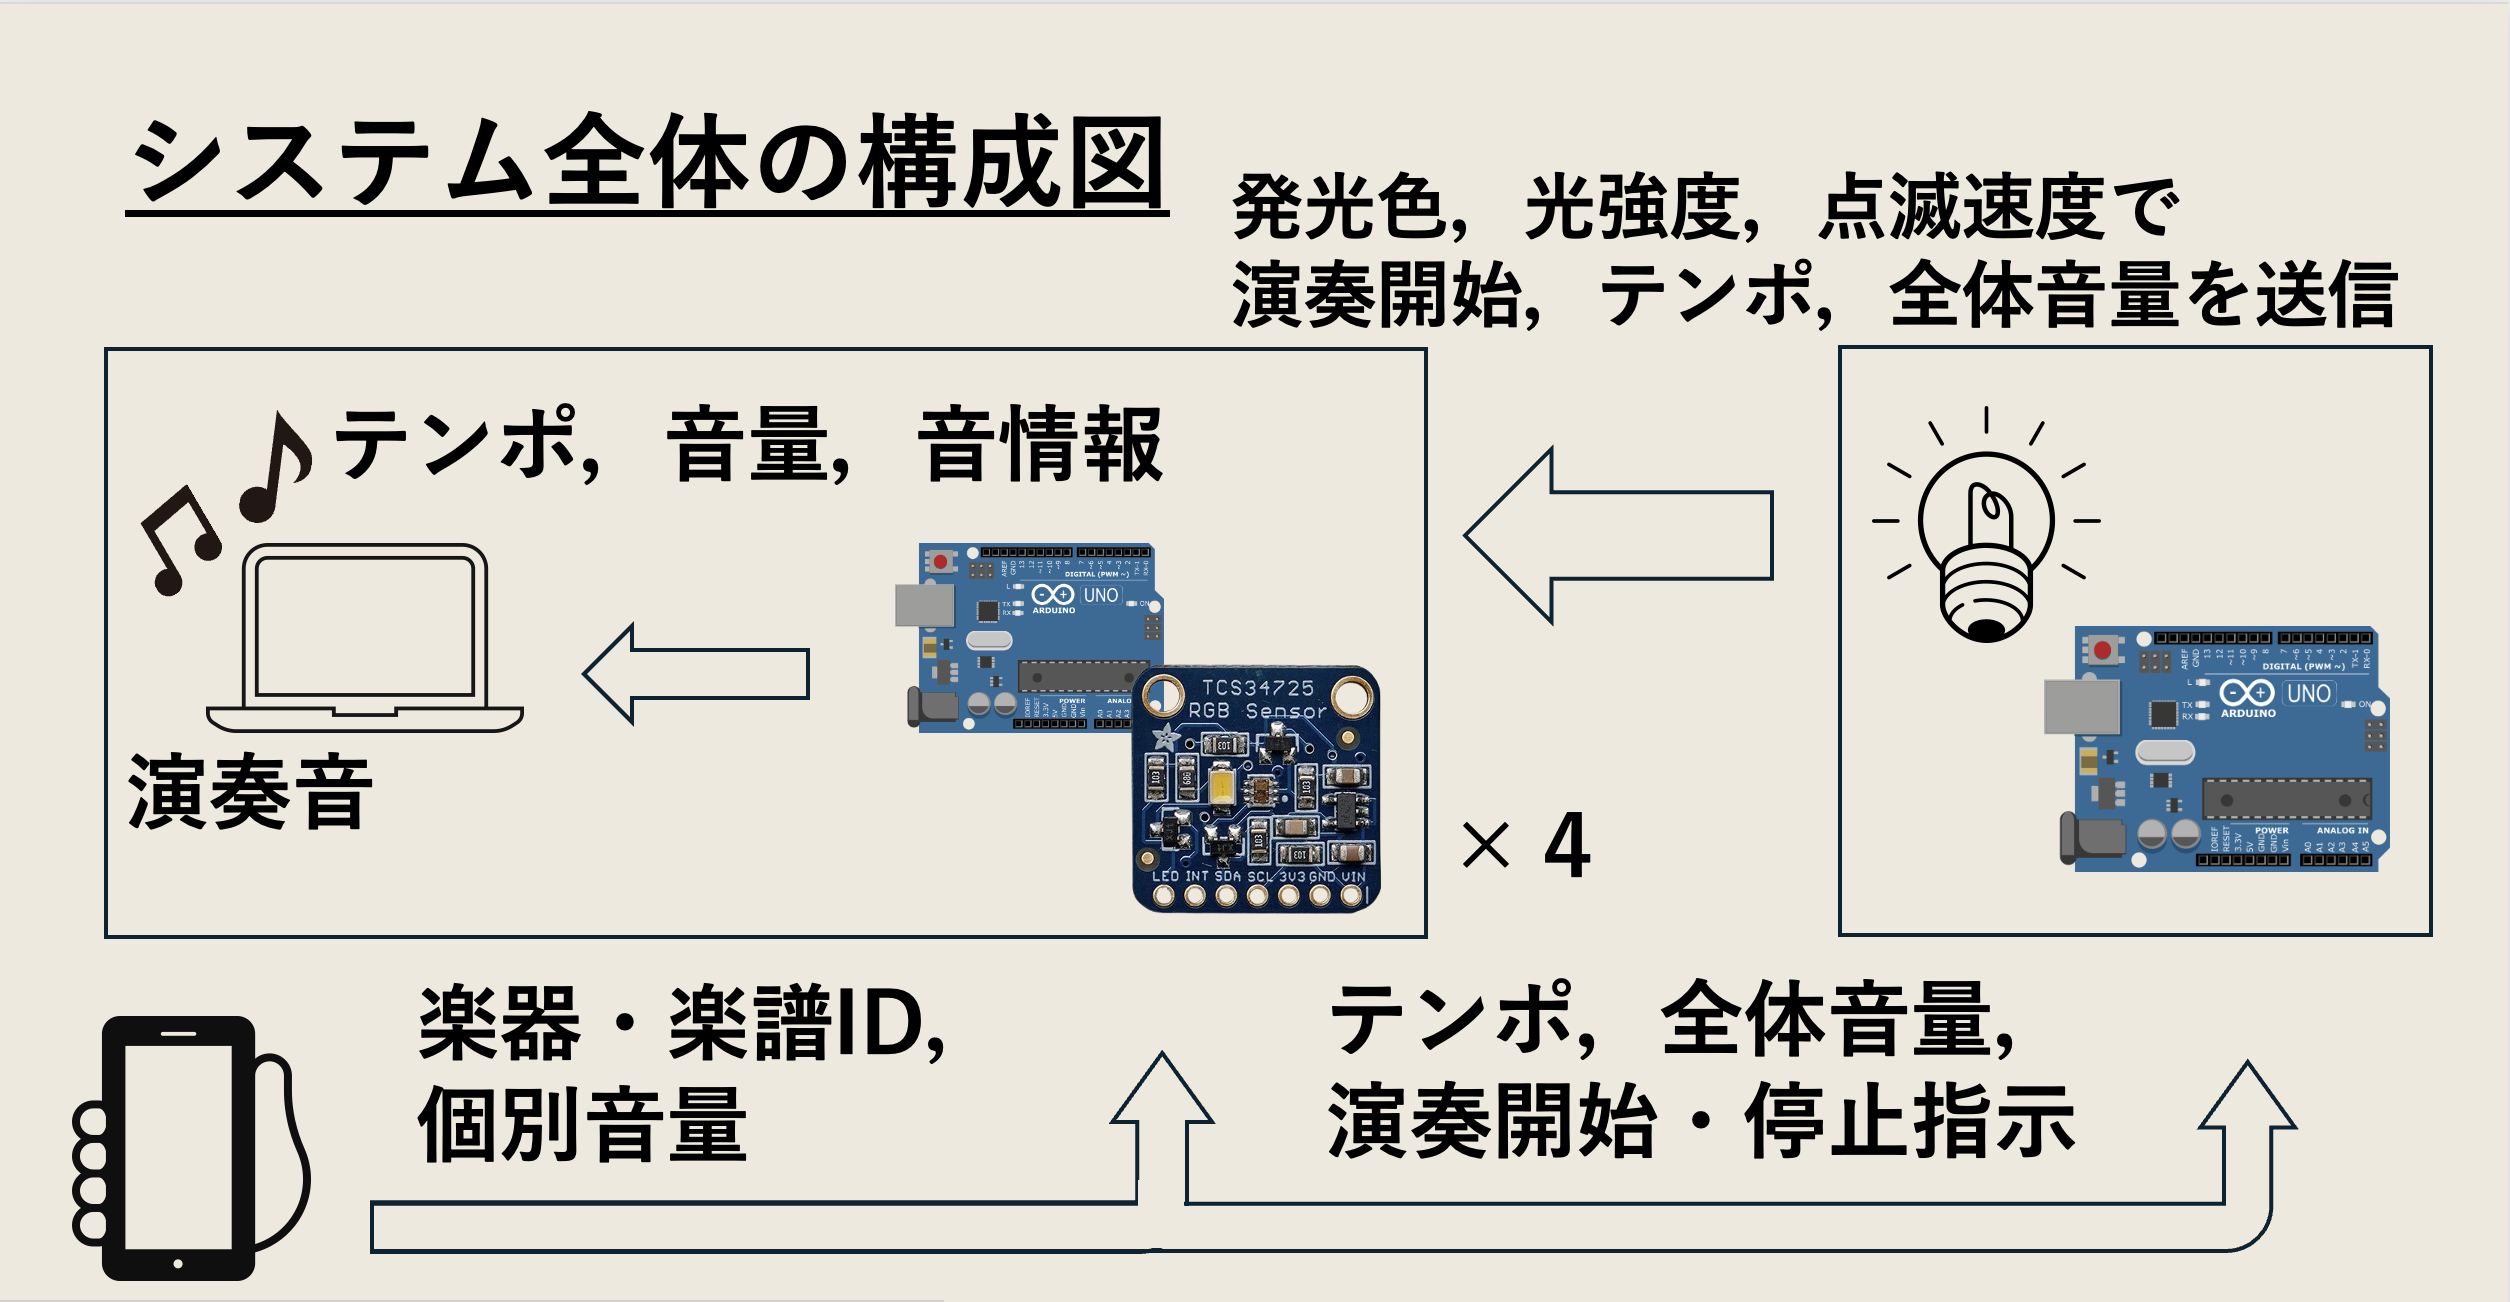
\includegraphics[width=140mm]{./img/構成図.png}
    \caption[system_overview]{指揮者および演奏者デバイスの構成図}
    \label{fig:system_overview}
  \end{center}
\end{figure}

また，本システムのLED通信部の指揮者，演奏者Arduinoの回路図を図\ref{fig:schematic}に示す．
指揮者デバイスでは，フルカラーLED赤，青，緑のピンをArduinoのD9，D10，D11ピンへ接続し，PWM制御によって発光色及び光強度を制御する．
演奏者デバイスでは，カラーセンサとI2C通信を行うため，Arduinoで用意されているSDA，SCL，電源，2つのGNDピンを用いて受光機能を実現する．
このとき，電圧はカラーセンサごとの最大電圧に応じて決定する．
\begin{figure}[H]
  \begin{center}
    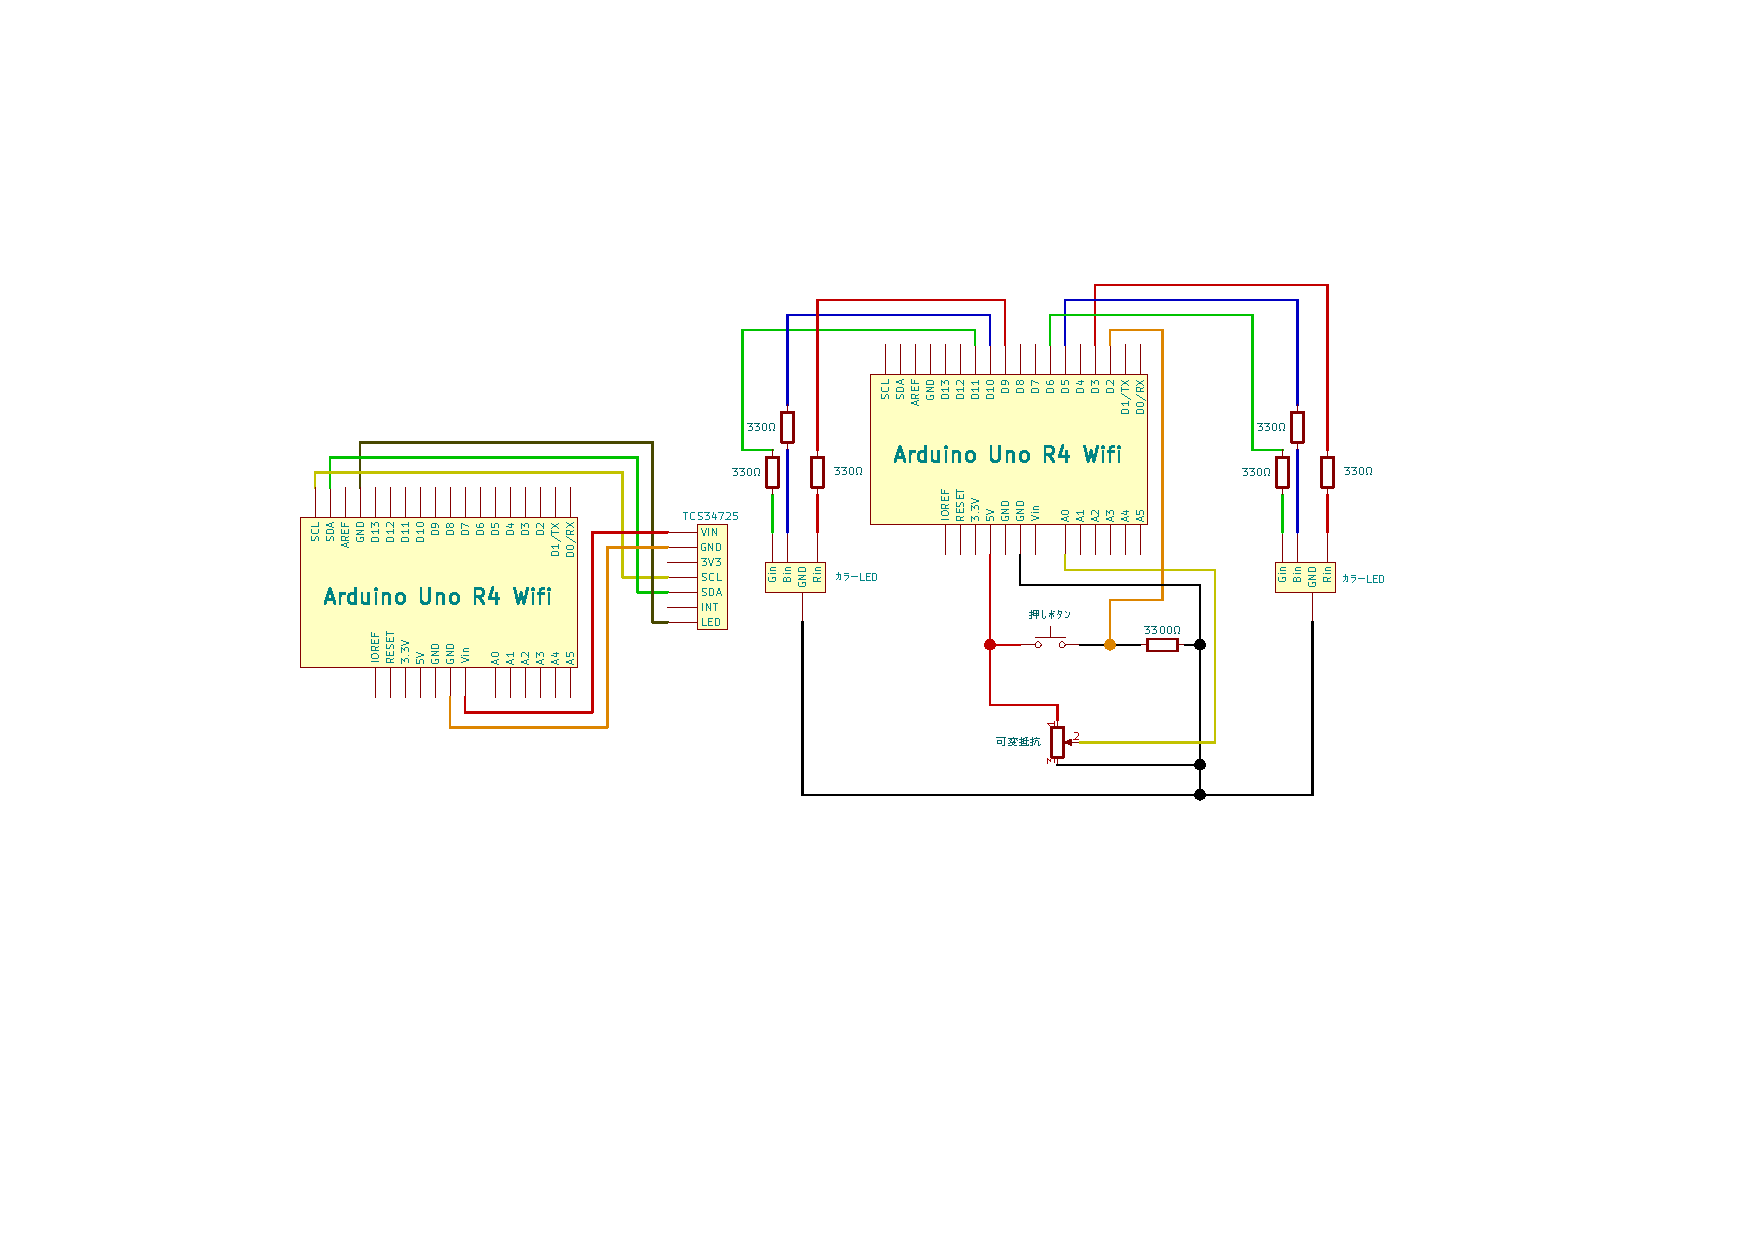
\includegraphics[width=140mm]{./img/LED点滅・受光回路(外部LEDピン対応修正)訂正版.pdf}
    \caption[schematic]{指揮者および演奏者デバイスの回路図}
    \label{fig:schematic}
  \end{center}
\end{figure}
各デバイスの主制御には，内蔵LEDマトリクスを備えたArduino Uno R4 WiFiを採用し，それぞれの役割に応じた回路で構成する．

指揮者デバイスの回路構成は，システム制御のための入力インターフェースと，信号送出のための出力インターフェースによって
形成される．物理的な起動・停止を制御するスイッチは，Arduinoの5VとGNDの間に接続し，スイッチとGNDの間にD2ピンを接続する．また，Web UIと同様に機能する
可変抵抗は，両端の端子を5VおよびGNDに，中央の端子をA0ピンに接続し，分圧された電圧値をテンポ情報として読み取る構成とした．
光信号の送出を担う4ピン仕様のフルカラーLEDは，GNDに加え，過電流防止用の330Ωの抵抗を介して信号入力端子をD9（赤），D11（緑），D10（青）ピンへ接続することで，
一つのLEDによる色彩および光量制御を実現している．

本システムはカラーセンサの色検知精度を向上させるため，
センサ周辺を箱で遮光する設計としている．そのため，
指揮者LEDが箱の内部に収まり，以下の2つの問題が生じる．
第一に，利用者が発光状態を視認できず，システムの動作状況を
把握しにくい．第二に，テスト時にLEDの発光タイミングを
カメラで捉えられず，遅延時間の計測が困難である．
これらの問題に対応するため，箱の外部にも同一の発光制御を行う
2個目のフルカラーLEDを追加する．
信号入力端子をD3（赤），D5（青），D6（緑）ピンへ
1個目のLEDと同様に330Ωの抵抗を介して接続する．

一方，演奏者デバイスの回路構成は，受光および視覚的フィードバックに特化した設計となっている．
指揮者側からの光信号を検知するカラーセンサは，I2C通信インターフェースを利用して接続される．
具体的には，モジュールのVINおよびGNDをArduinoの5VおよびGNDへ接続し，SDAおよびSCLピンをそれぞれの通信専用ピンへと
結線している．またモジュールのLEDもモジュールに付属しているLEDが発光するのを防ぐため，GNDに接続している．
%%%%%%%%%%%%%%%%%%%%%%%%
%%%%%%%%%%%%%%%%%%%%%%%%
\section{ソフトウェア設計}
% 全体のフローチャート ソフトでの処理 処理の種類 ex. 同期のテンポとLED発光 led受信制御(RGBによる制御) 受信による出力(LEDマトリクス，Prcoessingへの送信) Processingでの音再生
% データフロー図 同期演奏のデータフロー(何の情報が通信で渡るのか)
% ソフトウェア構成図
% データ設計 どんなデータをどうやって管理するのか
% 通信仕様
%%%%%%%%%%%%%%%%%%%%%%%%
\subsection{ファイル構成}
% 指揮者　演奏者 processingの三種類
% ファイル名，用途(演奏者，指揮者，楽器再生)，処理内容
本システムのソフトウェアは，
指揮者デバイス，
演奏者デバイス，
およびPC上で動作する音声再生プログラム，
Webサイトでの演奏制御プログラム
の4種類によって構成される．
各プログラムの主要ファイルを表\ref{tab:file_config}に示す．
\begin{table}[H]
\centering
\caption{ソフトウェアのファイル構成}
\label{tab:file_config}
\resizebox{\textwidth}{!}{

\begin{tabular}{|l|l|l|}
\hline
\textbf{ファイル名} & \textbf{動作環境} & \textbf{主な処理内容} \\ \hline

conductor.ino
& 指揮者Arduino
& BPM取得，LED発光制御，演奏開始・停止制御，Web受信処理を行う． \\ \hline

playerRGBMethod.ino
& 演奏者Arduino
& カラーセンサによる光信号受信，色判定，音情報のシリアル送信，Web受信処理を行う． \\ \hline

soundPlayer.pde
& Processing
& Arduinoから受信した音情報に基づき，楽器音の再生および制御を行う． \\ \hline

lyrics.h
& 演奏者Arduino
& LEDマトリクスに表示する歌詞データ，楽譜データを管理する． \\ \hline

index.html & PC & 利用者が楽器やテンポ等の演奏パラメータを選択するための操作画面を定義する． \\ \hline
script.js & PC & 送信ボタン押下時に設定値をJSON形式でサーバーへ送信する処理を担う． \\ \hline
server.js & PC & Node.js環境で動作し，ブラウザからの要求を各Arduinoへ中継する． \\ \hline

\end{tabular}
}
\end{table}
%%%%%%%%%%%%%%%%%%%%%%%%
\subsection{通信設計}
\subsubsection{LED通信}
指揮者Arduinoと演奏者Arduino間での通信の内容と方法を示す．
この区間での通信内容は，表\ref{tab:led_data}のようにLEDの点滅によるテンポ，点灯時のピーク時の光量による全体音量，LEDの発光色による演奏者Arduinoごとの開始タイミングである．
% \begin{table}[H]
%   \centering
%    \caption{送信内容} \label{tab:led_data}
%    \scalebox{0.55}{
%     \begin{tabular}{|l|l|l|} \hline
%       通信データ & 通信方法 & 処理\\ \hline
%       テンポ(bpm) & 指揮者の保持するbpmに応じてLEDを点滅& 前回，LED全体の光量が閾値を超えたときとの時間差で計算 \\\hline
%      全体音量 & カラーセンサで取得する光量clear値で音量決定 & LEDを最大の値で点灯させ，受光側のRGB値の最大値を初期化．点滅ごとの光量に応じて音量を変更\\\hline
%       Arduinoごとの開始タイミング & 特定のLEDの色を演奏者の開始タイミングとして設定 &紫，赤，青，緑をピアノ，バイオリン，フルート，ドラムに対応させ，受光した次のLED点滅から音再生 \\ \hline
%     \end{tabular}
%   }
% \end{table}
\begin{table}[H]
  \centering
  \caption{LED通信内容}
  \label{tab:led_data}
  \renewcommand{\arraystretch}{1.3}
  \begin{tabular}{|p{3cm}|p{4cm}|>{\raggedright\arraybackslash}p{7cm}|}
    \hline
    送信データ & LED表現 & 受信側処理 \\\hline
    テンポ(bpm)&指揮者の保持する bpm に応じてLED を点滅&前回 LED 全体の光量が閾値を超えたときとの時間差で計算する．\\ \hline
    全体音量 & 音量を光量で制御する． &
    ピーク時のCLEAR値をCLEAR\_MAX\_LOWからCLEAR\_MAX\_HIGHの範囲で20〜100にリスケーリングし，個別音量倍率をかけて音量を算出する．
    \\ \hline

    Arduino ごとの開始タイミング
    &
    特定の LED の色を
    演奏者の開始タイミングとして設定する．
    &

    紫，赤，青，緑を受光したRGB値の閾値で判別し，
    各色に対応するArduinoを識別する．
    自身の担当色を検出したArduinoが，Webサイトから
    事前に受信した楽器IDに従って音再生を開始する．\\ \hline

  \end{tabular}
\end{table}
\subsubsection{シリアル通信}
演奏者Arduinoと楽器演奏用のProcessing間での通信の内容と方法を示す．
送信内容は，表\ref{tab:serial_data}のように，楽器変更，音再生のために音高，音量，音の長さ，楽器IDを送信する．
この区間の通信はArduinoとProcessing側のPCをUSB Type-Cで繋げ，シリアル通信を行う．
シリアル通信の送受信は，データ転送レートbps(baud)を合わせる．
送信はserial.write(buf,len)を用いて行う．
Serial.writeは1 Byteずつデータを送ることができ，本送信データは合計4 Byte以下であるため，4つの1 Byte配列で送信する．
そのため，図\ref{fig:serial_bit}のように，通信データをビットシフトで非負32 bit整数に入れ込み，バイト配列に入れていく．
受信は，SerialEvent関数を用いて4 Byte受け取ったら，データを取り出し音を再生する．

\begin{table}[H]
  \centering
   \caption{送信内容} \label{tab:serial_data}
   \scalebox{0.75}{
    \begin{tabular}{|l|l|l|} \hline
      送信データ & 送信内容 & 送信ビット数 \\ \hline
      音高(pitch) & ドレミファソラシドを(0-31)に対応し送信 & 6 bit \\\hline
      音量(volume) & 音量を(0-100)で送信 & 7 bit \\ \hline
      音の長さ(duration) & 一音の長さを(0-4095)msで送信 & 12 bit \\\hline
      楽器ID(instrumentData) & ピアノ・バイオリン・フルート・パーカッションを(0-3)に対応し送信 & 2 bit \\\hline
    \end{tabular}
  }
\end{table}
\begin{figure}[H]
  \begin{center}
    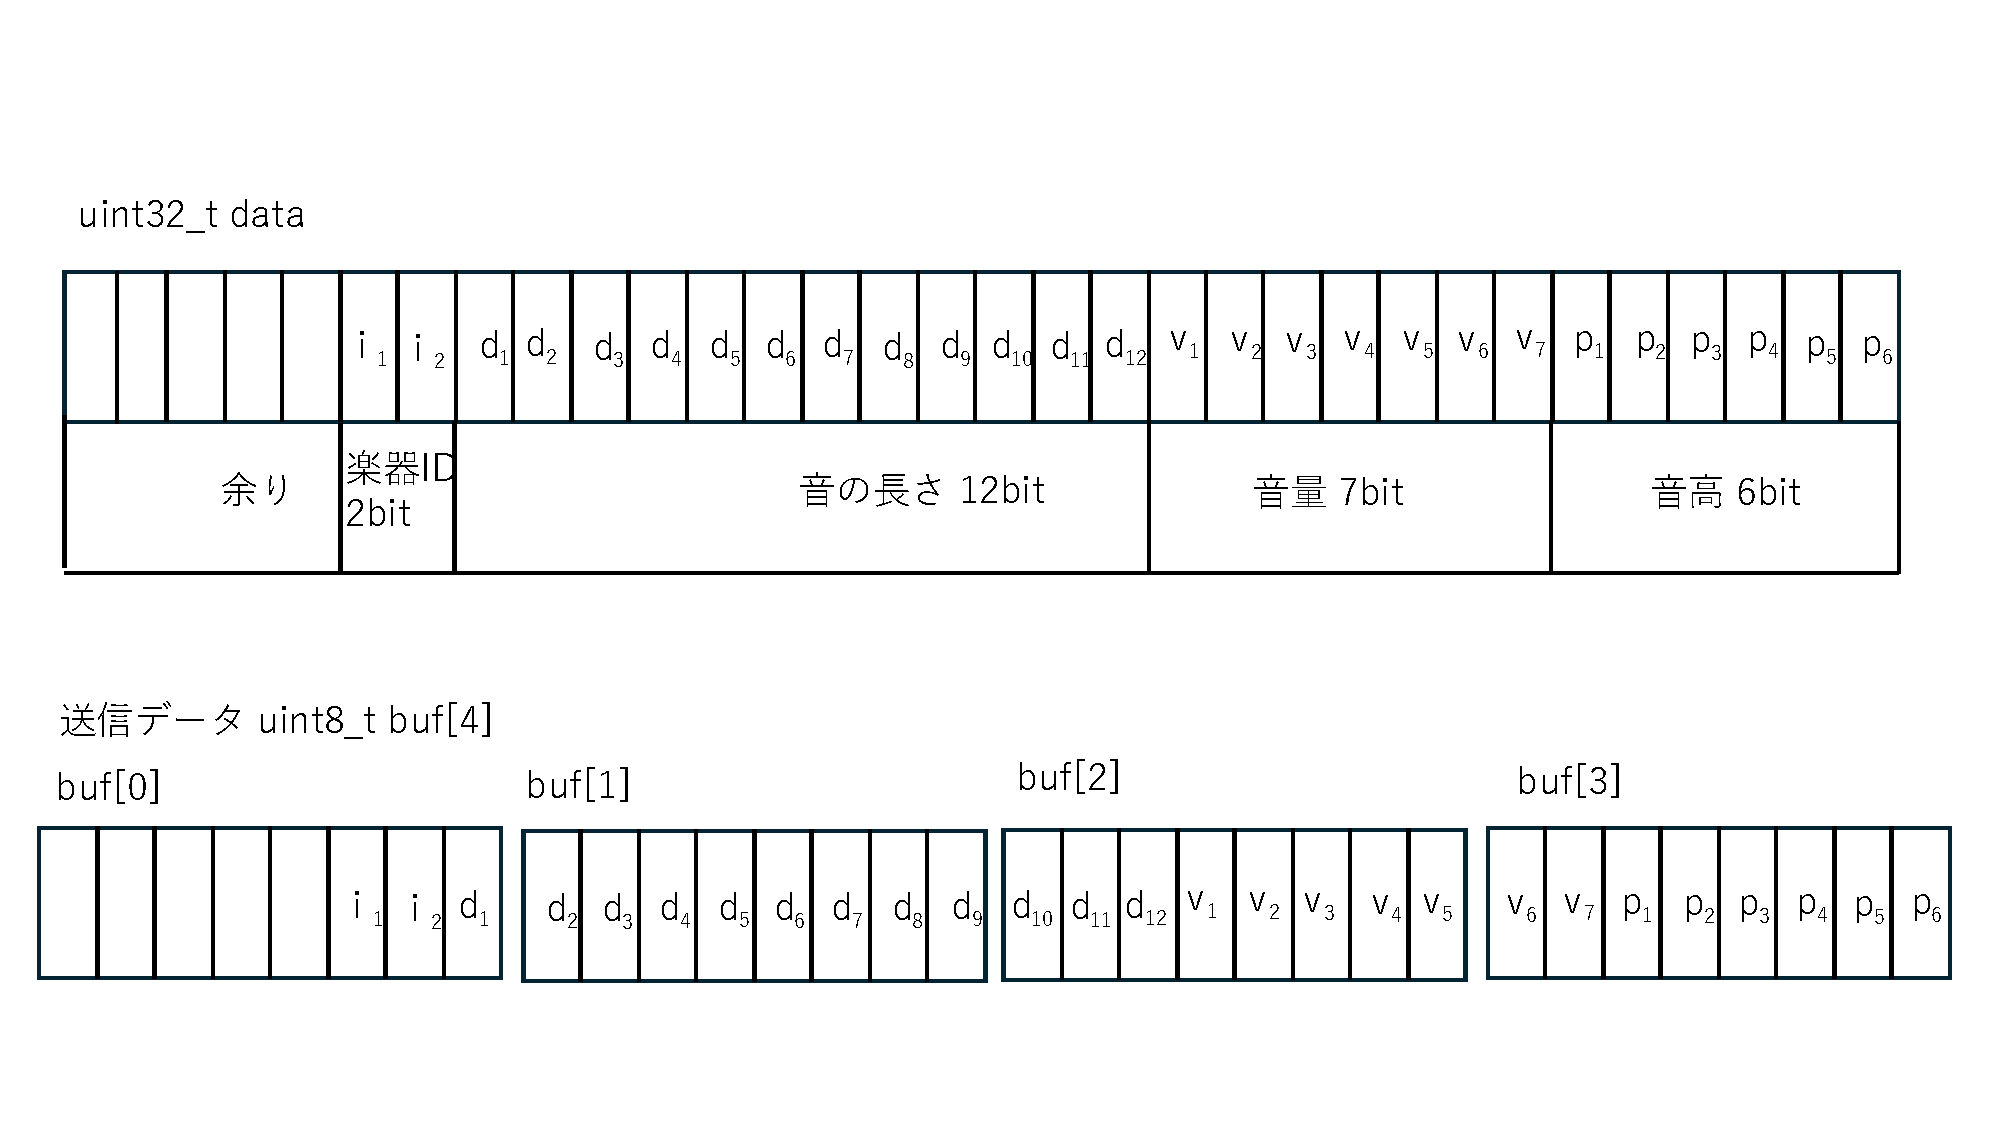
\includegraphics[width=140mm]{./img/serial_bit.pdf}
    \caption[serial_connection]{Byte配列での送信方法}
    \label{fig:serial_bit}
  \end{center}
\end{figure}
% \begin{table}[H]
%   \centering
%    \caption{送受信で用いる関数} \label{tab:serial_func}
%    \scalebox{0.75}{
%     \begin{tabular}{|l|l|l|} \hline
%       送信/受信 & 関数名 & 仕様 \\ \hline
%       双方 & serial.begin(baud) & baudを共通し，シリアル通信を行う際双方のビットレートを合わせる． \\\hline
%       送信 & serial.write(buf,len) & バイト配列をlenの個数分送信する．\\\hline
%       受信 & void serialEvent(serial p) & データが使用可能になったときに呼び出される． \\ \hline
%     \end{tabular}
%   }
%   \end{table}
\subsection{LEDマトリクスへの歌詞表示}
エンターテイメントとして演奏者Arduinoに現在の再生している音に対応した歌詞を表示させる．
データは演奏者Arduinoが保持し，表示内容は図\ref{fig:ledMatrixDesign}のようにArduinoのLEDマトリクスへカタカナを表示させる．
表示タイミングは全体の演奏の遅延を考慮して，演奏者ArduinoからProcessingへ音情報を送信した後に歌詞を表示させる．
データとしては，表\ref{tab:matrixData}のように各文字ごとの配列と曲全体の歌詞配列を持つ．
このとき，歌詞データは楽譜情報と同じ要素数を持ち，同じインデックスを共有して使用する．
それぞれの文字は，定数で32ビットの符号なし整数型であり，16進数の3要素でLEDマトリクスの96 bitを表現している．
マトリクスをコード内で使用するために必要な関数などを表\ref{tab:matrixCode}に示す．
LEDマトリクス用のヘッダファイルと楽譜情報の入ったlyricsヘッダファイルをインクルードし，オブジェクトを作成する．
セットアップ関数内でSerial.beginを呼び出し，matrix.loadFrame関数で表示する．
\begin{figure}[H]
  \begin{center}
    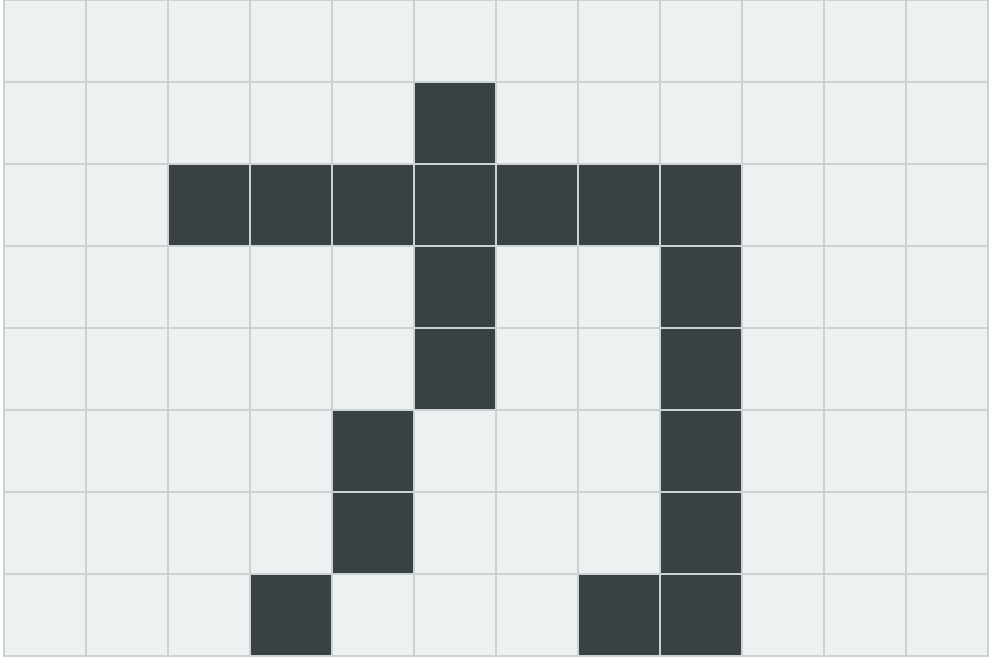
\includegraphics[width=100mm]{./img/matrixOneText.png}
    \caption[LEDマトリクス1文字ずつ表示]{LEDマトリクスに1文字ずつ表示} 
    \label{fig:ledMatrixDesign}
  \end{center}
\end{figure}

\begin{table}[H]
  \centering
   \caption{歌詞データ} \label{tab:matrixData}
   \scalebox{0.75}{
    \begin{tabular}{|l|c|l|l|} \hline
      型 & 配列名 & 要素内容 & データ \\ \hline
      const uint32\_t  & ka[3] & カタカナの「カ」& 0x201f, 0xc0240240, 0x4404408c \\\hline
      const uint32\_t  & e[3]  & カタカナの「エ」& 0x1f004, 0x400400, 0x400403f8 \\\hline
      const uint32\_t\textasteriskcentered  & lyrics[] & カエルの歌全体の歌詞 & {ka, e, ru,..} \\\hline
    \end{tabular}
  }
\end{table}

\begin{table}[H]
  \centering
   \caption{LEDマトリクスを使用するためのコード} \label{tab:matrixCode}
   \scalebox{0.75}{
    \begin{tabular}{|l|l|l|} \hline
      コード & 場所& 内容 \\\hline
      \#include "Arduino\_LED\_Matrix.h" & コード先頭& LEDマトリクスを使用するためのヘッダファイル \\ \hline
      \#include "lyrics.h" &コード先頭 & 歌詞データを格納したヘッダファイル\\\hline
      ArduinoLEDMatrix matrix & コード先頭 & オブジェクトを作成 \\\hline
      matrix.begin() & setup関数内 & LED Matrixを開始 \\\hline
      matrix.loadFrame(lyrics[index]) & loop関数内 &  表示させたい文字配列を引数で指定し表示する．\\\hline
    \end{tabular}
  }
\end{table}

\subsection{音生成・再生}
楽器音はProcessingのオーディオライブラリMinimを使用し，
各楽器の音色特性に応じて，波形，倍音，ノイズ成分，エンベロープを
組み合わせて生成する．

ピアノ・バイオリン・フルートの音色生成には加算合成を用いる．
加算合成とは，複数のサイン波（基音および倍音）を重ね合わせることで
任意の音色を表現する手法であり，出力波形$y(t)$は式(\ref{加算合成})で表される．

\begin{equation}
  y(t) = \sum_{n=1}^{N} A_n \sin(2\pi n f_0 t)
  \label{加算合成}
\end{equation}

ここで，$f_0$は基音周波数，$n$は倍音次数，$A_n$は各倍音の振幅である．
$A_n$の組み合わせを楽器ごとに変えることで音色の違いを表現する．
パーカッションはノイズ成分と低周波サイン波を組み合わせて打撃音を生成する．

各楽器の倍音構成$A_n$は，実際の楽器音の録音データに対して
FFT（高速フーリエ変換）を適用し，得られた周波数スペクトルから
基音および各倍音成分の振幅を読み取ることで決定する．
また，録音データ全体の振幅を解析し，
Attack，Decay，Sustain，Releaseの各パラメータを取得する．
取得したADSRパラメータは，振幅の時間変化として波形生成に反映する．

\subsection{受光機能}

\subsubsection{点滅間隔計測}
LEDの点滅間隔を計測することで，演奏テンポの取得を行う．
clear値が閾値を超えた時刻を記録し，連続する2回の検出時刻の差を点滅間隔として算出する．
この値を演奏タイミング制御へ利用する．

図\ref{fig:点滅間隔}に点滅間隔計測の概要を示す．

\begin{figure}[H]
  \begin{center}
    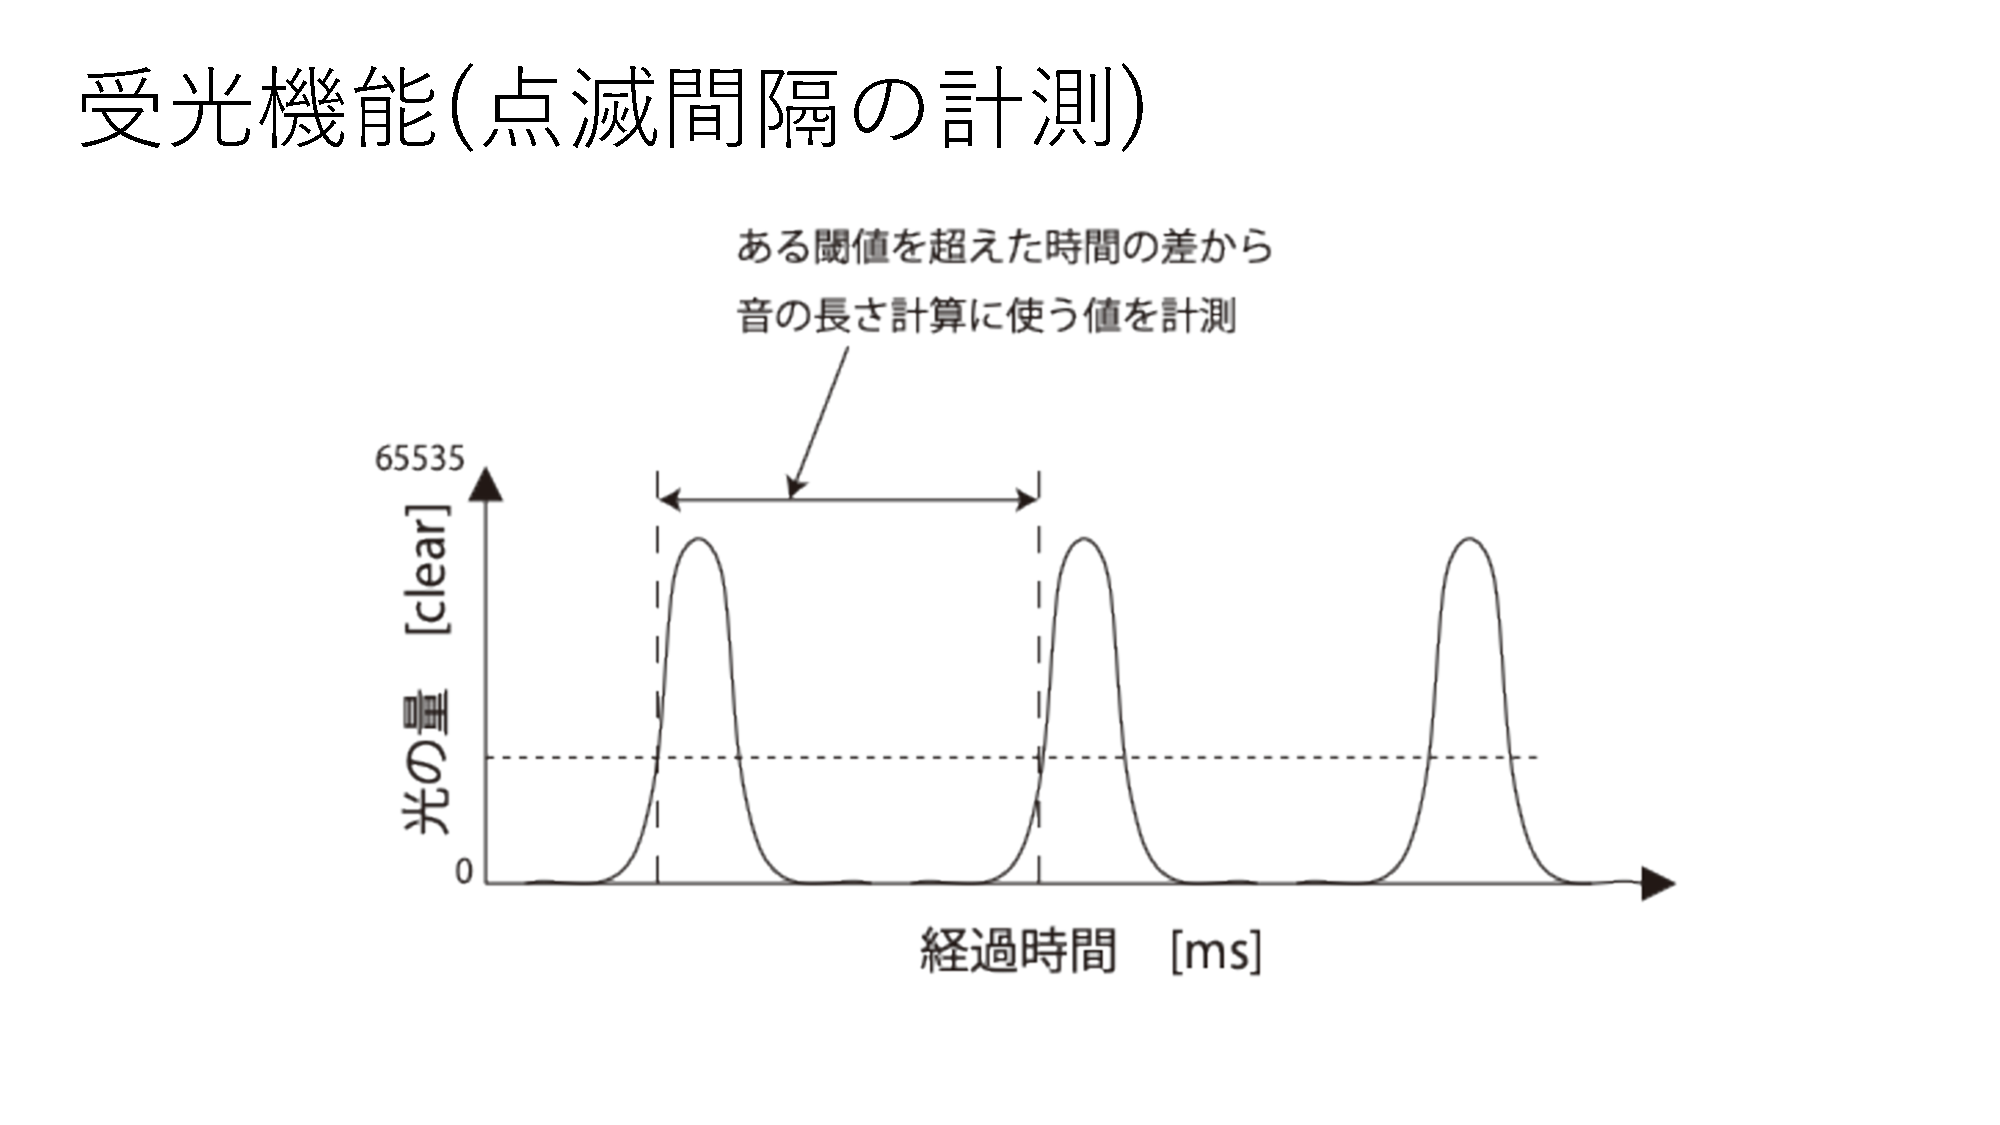
\includegraphics[width=140mm]{./img/点滅間隔.pdf}
    \caption[点滅間隔]{点滅間隔計測の概要}
    \label{fig:点滅間隔}
  \end{center}
\end{figure}

\subsubsection{光量ピーク検出}
受光した光量値の最大値を利用することで，演奏音量の制御を行う．
受光した光が強いほど大きな音量，弱いほど小さな音量となるように設定することで，光強度に応じた演奏表現を可能とする．

図\ref{fig:最大値}に光量最大値計測の概要を示す．

\begin{figure}[H]
  \begin{center}
    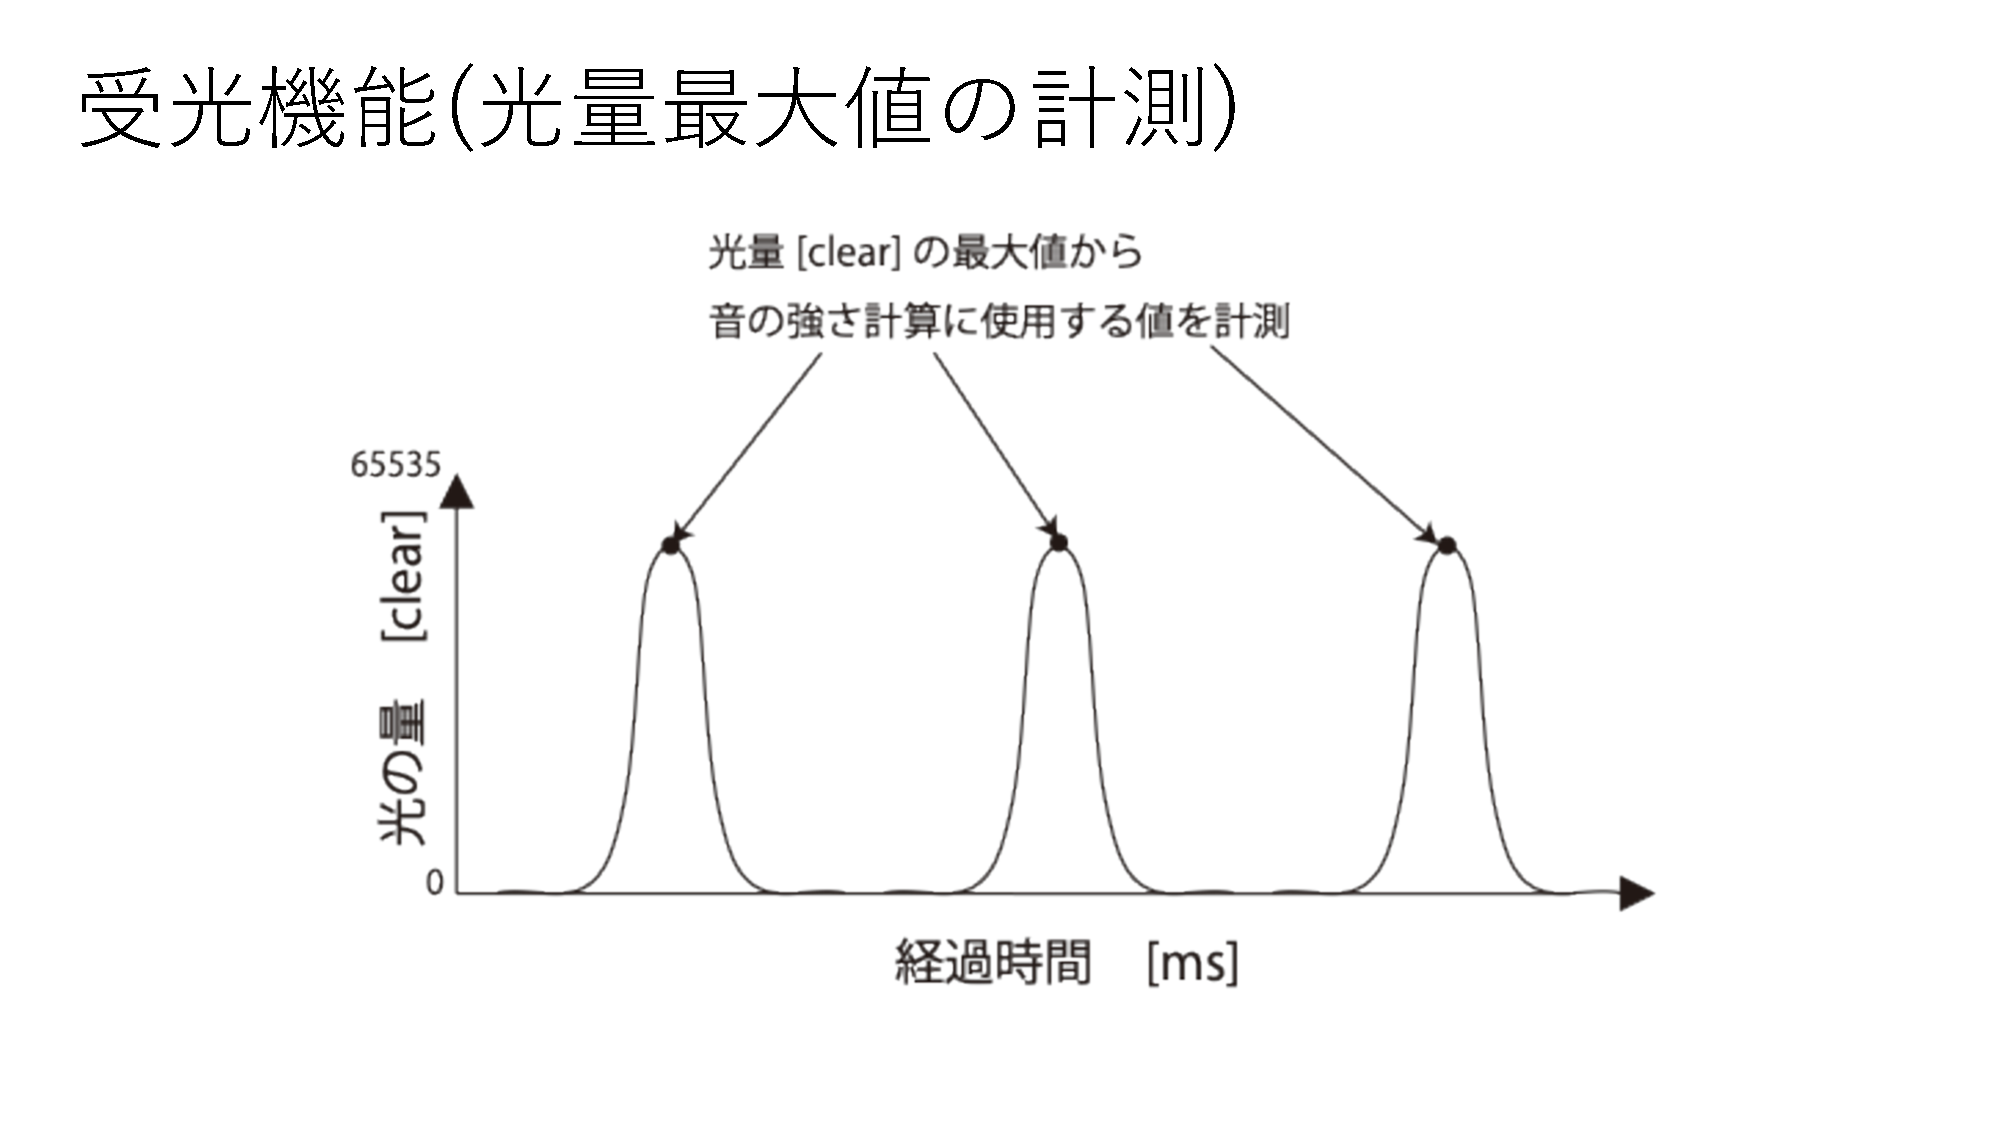
\includegraphics[width=140mm]{./img/最大値.pdf}
    \caption[最大値]{光量最大値計測の概要}
    \label{fig:最大値}
  \end{center}
\end{figure}


\subsubsection{発光色の識別}
カラーセンサから取得したRGB値を用いて，発光色の識別を行う．
本システムでは赤・緑・青・紫の4色を使用し，各色に異なるArduinoを割り当てる．
演奏者Arduinoは割り当てられた色を検出したら，演奏を開始する．
一度自色を検出した後は，以降の点滅に対して色判定を行わず点滅検出のみで楽譜を進行させる．
色の判定はRGB値そのものではなく，図\ref{fig:rgb_ratio_calc}に示すように各成分の割合（R/(R+G+B)など）が事前測定により決定した閾値を上回るか下回るかによって行う．
具体的には，R成分の割合が閾値以上かつG・B成分の割合が閾値以下の場合を赤と判定するなど，
各色に対応するRGB割合の条件を図\ref{fig:rgb_ratio_measure}に示す方法で事前測定により決定し，色識別を行う．

\begin{figure}[H]
  \begin{center}
    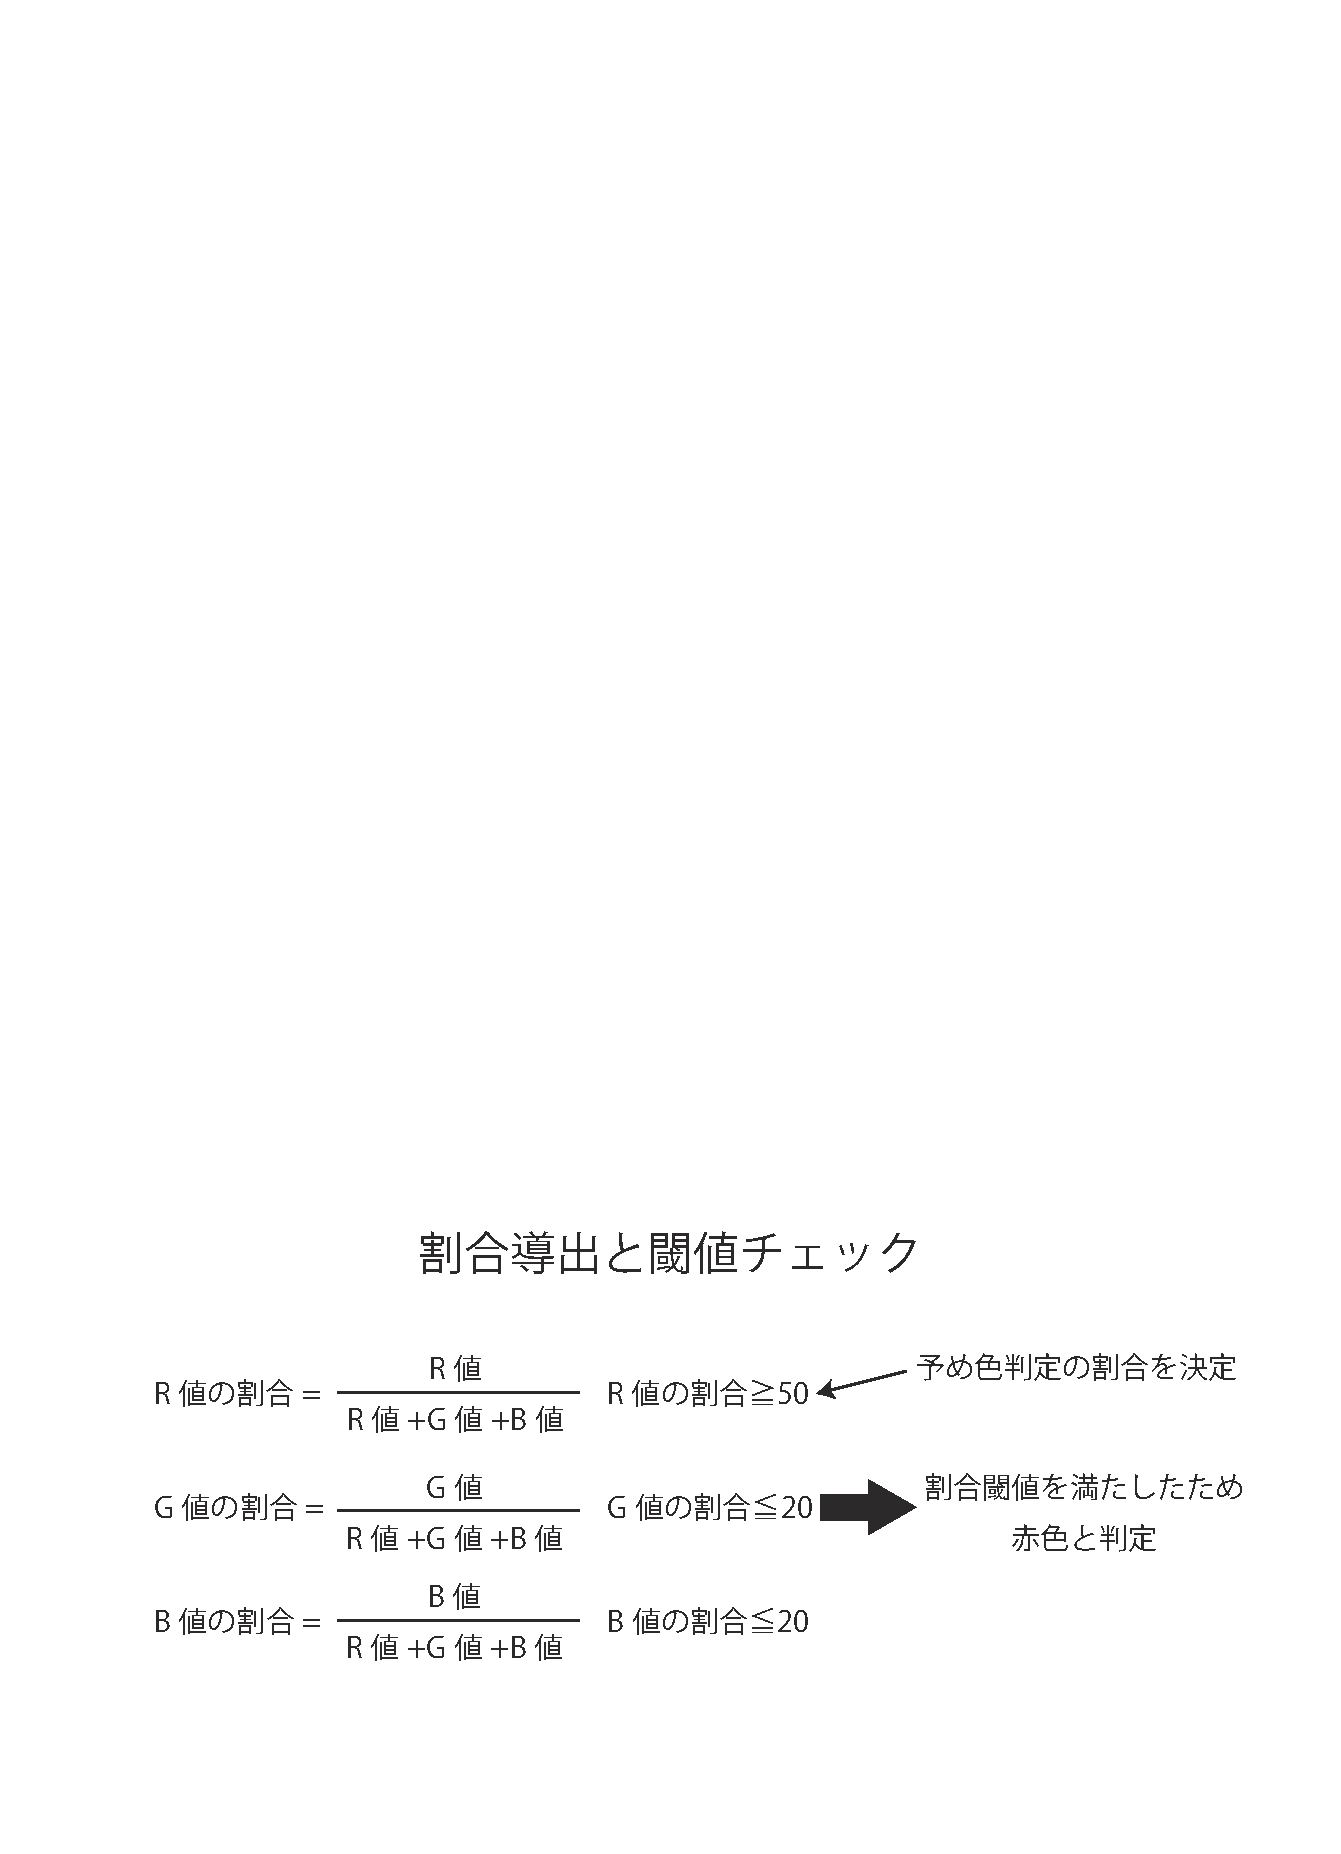
\includegraphics[width=140mm]{./img/ハッカソンRGB割合計算図.pdf}
    \caption[RGB割合計算]{RGB割合の計算方法}
    \label{fig:rgb_ratio_calc}
  \end{center}
\end{figure}

\begin{figure}[H]
  \begin{center}
    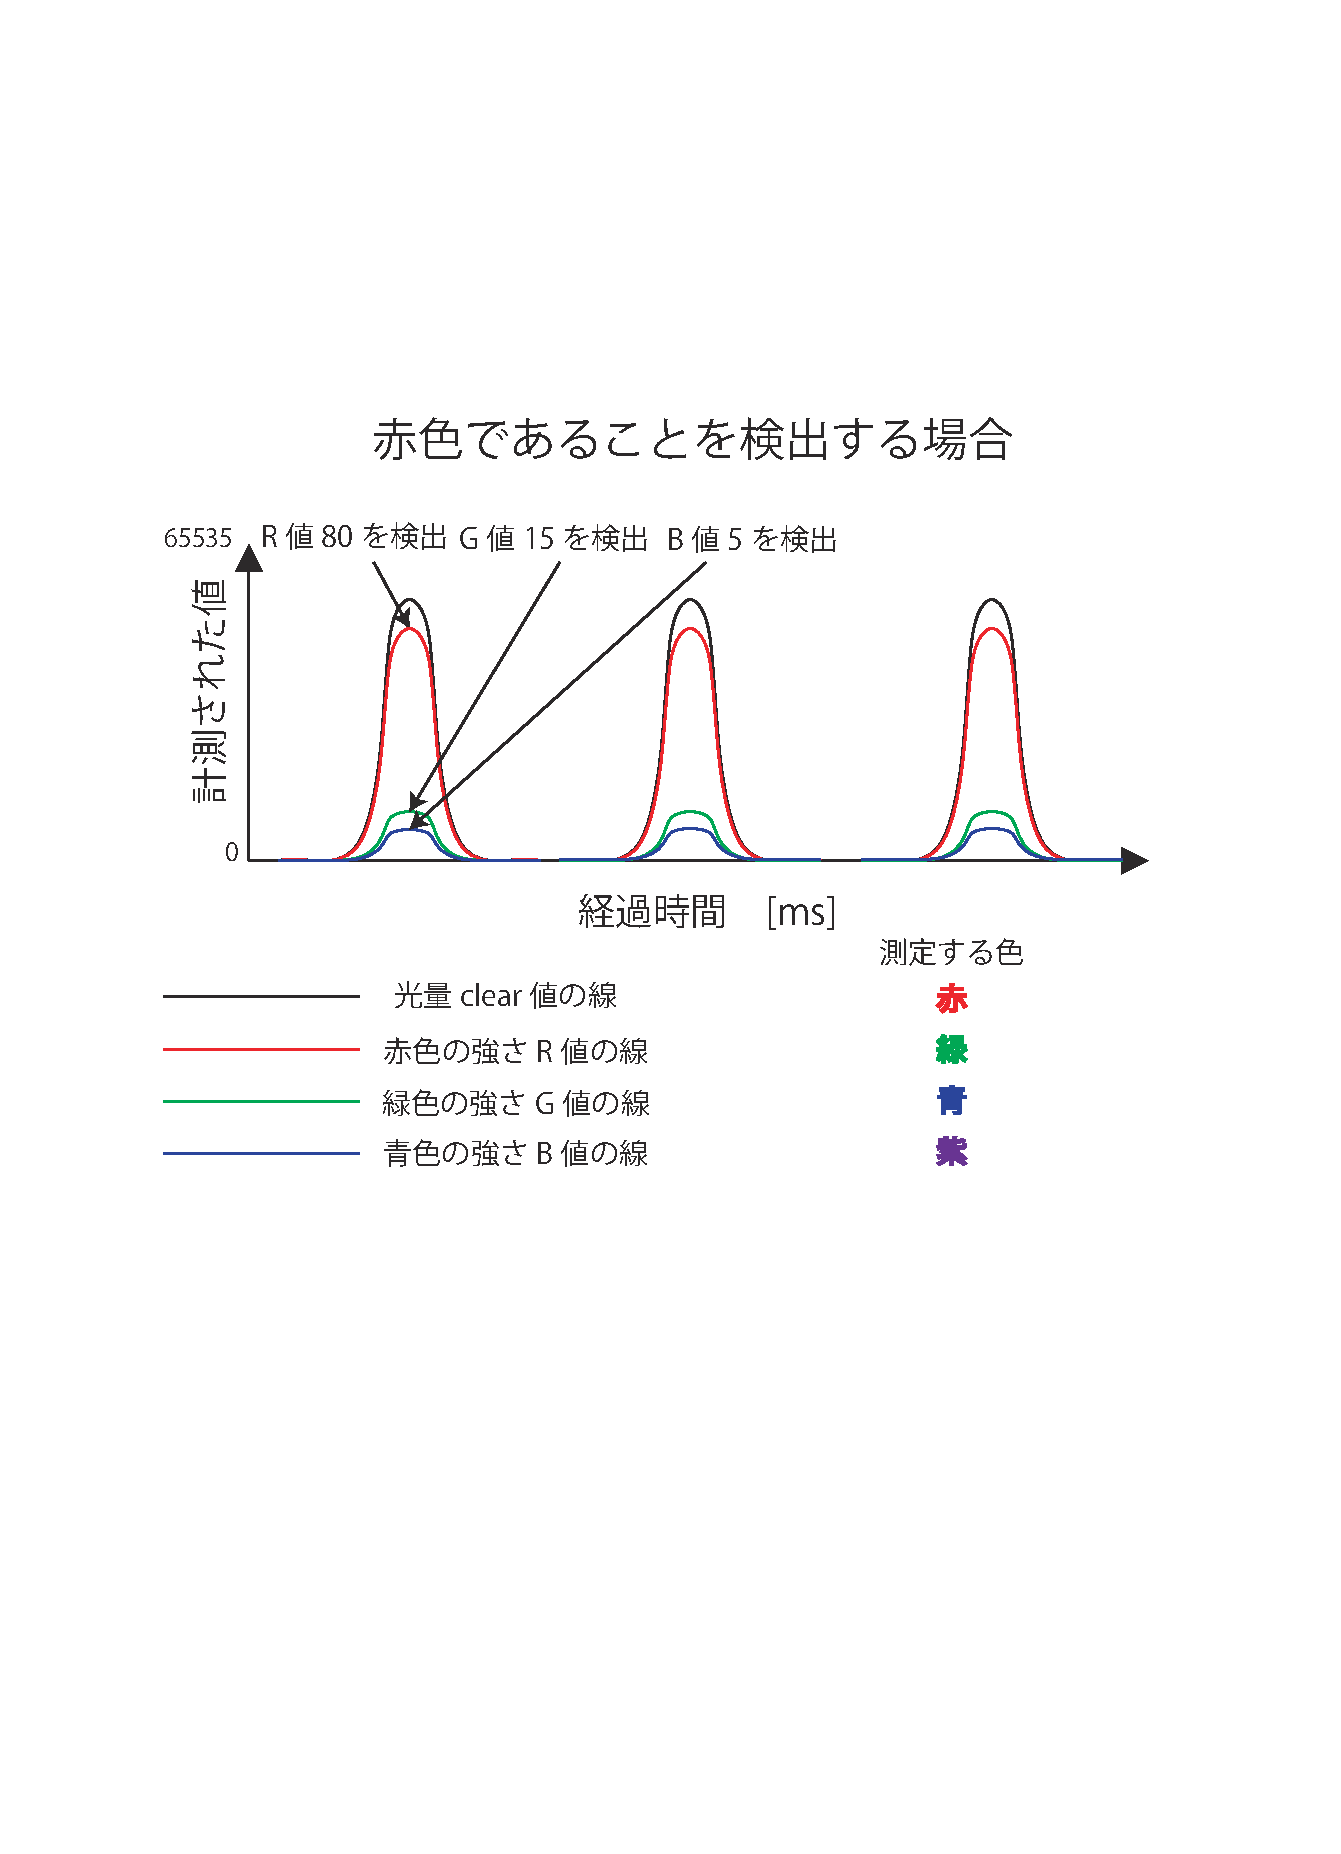
\includegraphics[width=140mm]{./img/ハッカソンRGB割合計測図.pdf}
    \caption[RGB割合計測]{RGB割合の計測方法}
    \label{fig:rgb_ratio_measure}
  \end{center}
\end{figure}

\section{スイッチによる入力制御の詳細設計}
本節では，指揮者デバイスにおける物理入力，すなわち演奏の起動・停止を担うタクトスイッチと，
予備系統としてテンポを制御する可変抵抗について，その具体的な入力制御の方法を述べる．
これらの入力は，図\ref{fig:system_config}に示すシステム構成のうち，指揮者Arduinoへの入力インターフェースに該当する．
以降の設計は，検証用に実装した指揮者デバイスの入力制御プログラム（\texttt{LED\_switch.ino}）の動作を基にしている．

\subsection{入力ピンの割り当てと初期設定}
指揮者デバイスでは，タクトスイッチ，可変抵抗，および同期用LEDをそれぞれ独立したピンに割り当てる．
各入力の接続および設定方法を表\ref{tab:input_pin}に示す．

\begin{table}[H]
\centering
\caption{指揮者デバイスの入力ピン割り当てと設定}
\label{tab:input_pin}
\begin{tabular}{|p{3.2cm}|p{2.2cm}|p{8.0cm}|}
\hline
入力要素 & ピン & 設定および接続方法 \\ \hline
タクトスイッチ & D2 & \texttt{INPUT\_PULLUP} に設定し，内部プルアップ抵抗を有効化する．スイッチの他端をGNDへ接続し，外付け抵抗を不要とするとともにノイズによる誤検出を抑制する． \\ \hline
可変抵抗 & A0 & \texttt{INPUT} に設定し，A/Dコンバータでアナログ電圧を読み取る．3端子の可変抵抗（ポテンショメータ）を用い，両端の端子を5V・GNDに，中央端子（ワイパ）をA0へ接続することで，可変抵抗自体が分圧器として機能し，ツマミ位置に応じた電圧をテンポ情報として取得する（\ref{subsec:voltage_divider}項参照）． \\ \hline
同期用LED &D9,D11,D10 & \texttt{OUTPUT} に設定し，\texttt{analogWrite} によるPWM制御で発光のON/OFFおよび光強度を制御する． \\ \hline
同期用LED（箱外） & D3,D5,D6 & 箱内LEDと同一の制御信号を出力する．利用者への視覚フィードバックおよびテスト時の遅延計測を目的として追加する． \\ \hline
\end{tabular}
\end{table}

タクトスイッチを \texttt{INPUT\_PULLUP} とすることで，スイッチが押されていないときは入力がHIGH，
押されたときにGNDへ落ちてLOWとなる．プログラム上では，押下を真として扱うために読み取り値を論理反転し，
「押下時に \texttt{true}」となる状態変数として保持する．

\subsection{可変抵抗によるテンポ入力}
可変抵抗から読み取ったアナログ値を，演奏テンポ（BPM）および同期用LEDの点滅間隔へ変換する．
A/Dコンバータは入力電圧を $0$〜$1023$ の整数値として出力する．
この入力値 $v$ を，演奏に用いるテンポ範囲 $30$〜$240$\,BPM へ対応させる．
変換後のBPM $B$ は式(\ref{eq:bpm_map})で与えられる．

\begin{equation}
  B = 30 + \frac{240 - 30}{1023}\, v
  \label{eq:bpm_map}
\end{equation}

得られたBPMから，同期用LEDが1回点滅する周期（点灯と消灯を合わせた時間）$T_{pulse}$\,[ms] を
式(\ref{eq:pulse})により算出する．
本設計では，1拍を2分割した8分音符の間隔で点滅させる．

\begin{equation}
  T_{pulse} = \frac{60000}{B \times 2}
  \label{eq:pulse}
\end{equation}

ここで，1回の点滅における点灯時間は，テンポによらず短い固定値 $T_{on}$（本設計では $20$\,ms）とし，
残りの時間 $T_{pulse} - T_{on}$ を消灯時間に充てる．
このように点灯時間を短縮することで，発光が鋭いパルス状となり，
受光側のカラーセンサが点滅（テンポ）を検出しやすくなる利点がある．

式(\ref{eq:bpm_map})・式(\ref{eq:pulse})により，可変抵抗のツマミ位置に応じてLEDの点滅間隔が連続的に変化し，
ネットワークを介さずに直感的なテンポ制御を可能とする．
可変抵抗の値はメインループ内で常時読み取られ，演奏中のリアルタイムなテンポ変更にも対応する．

\subsection{可変抵抗による分圧の原理}
\label{subsec:voltage_divider}
前項のテンポ入力を成立させるには，ツマミの操作に応じてA0ピンの電圧が連続的に変化する必要がある．
本設計では，図\ref{fig:voltage_divider}に示すように，3端子の可変抵抗（ポテンショメータ）を分圧器として用いる．

3端子の可変抵抗は，抵抗体の両端（端子1・端子3）と，抵抗体上を摺動するワイパ（端子2）からなる．
ワイパによって抵抗体は，端子1側の抵抗 $R_{a}$ と端子3側の抵抗 $R_{b}$ の2つに分割される．
ここで，端子1を電源電圧 $V_{cc}$（$5$\,V），端子3をGND，ワイパをA0ピンへ接続すると，
A0ピンの電圧 $V_{A0}$ は式(\ref{eq:divider})で与えられる．

\begin{equation}
  V_{A0} = V_{cc} \cdot \frac{R_{b}}{R_{a} + R_{b}}
  \label{eq:divider}
\end{equation}

ツマミを回すとワイパ位置が移動し，$R_{a}$ と $R_{b}$ の比が変化するため，
式(\ref{eq:divider})に従って $V_{A0}$ が $0$\,Vから $V_{cc}$ まで連続的に変化する．
このように，可変抵抗1つで分圧器が構成されるため，外付けの固定抵抗を別途追加する必要はない．
この電圧変化をA/Dコンバータで $0$〜$1023$ の値として読み取り，式(\ref{eq:bpm_map})によりBPMへ対応させることで，テンポの可変制御を実現する．

\begin{figure}[H]
  \centering
  \begin{tikzpicture}[
    line/.style={draw, thick},
    font=\footnotesize
  ]
    % 抵抗体（縦長の箱）
    \node[draw, thick, minimum width=0.8cm, minimum height=2.6cm] (pot) at (0,-2) {};
    % 端子1（上）= Vcc
    \draw[line] (0,-0.7) -- (0,-0.2);
    \node[above] at (0,-0.2) {端子1：$V_{cc}$ ($5$\,V)};
    % 端子3（下）= GND
    \draw[line] (0,-3.3) -- (0,-3.8);
    \node[below] at (0,-3.8) {端子3：GND};
    % ワイパ（中央）= A0
    \draw[line, -{Stealth[length=2mm]}] (1.6,-2) -- (0.42,-2);
    \node[right] at (1.6,-2) {端子2（ワイパ）：A0ピンへ};
    % 分割抵抗のラベル
    \node[left] at (-0.45,-1.35) {$R_{a}$};
    \node[left] at (-0.45,-2.65) {$R_{b}$};
  \end{tikzpicture}
  \caption{3端子可変抵抗（ポテンショメータ）による分圧}
  \label{fig:voltage_divider}
\end{figure}

\subsection{タクトスイッチによる起動・停止制御}
タクトスイッチは，押すたびに演奏の開始・停止が交互に切り替わるトグル動作とする．
ここで，スイッチを「押している間ON」とする単純な読み取りではなく，
「押された瞬間」のみを一度だけ検出してシステム状態を反転させる方式を採用する．
これは，1回の押下で複数回の切り替えが発生することを防ぐためである．

\subsubsection{押下エッジの検出}
押された瞬間を検出するため，直前のループでのスイッチ状態 $s_{prev}$ と
現在のスイッチ状態 $s_{now}$ の2つを保持する．
そして，$s_{prev}$ が非押下（\texttt{false}）かつ $s_{now}$ が押下（\texttt{true}）へ
変化した遷移を「押下の立ち上がりエッジ」として検出する．
この立ち上がりエッジが検出されたときにのみ，システム全体のON/OFF状態 $S_{sys}$ を反転させる．
ループの末尾で $s_{prev} \leftarrow s_{now}$ と更新することで，次回ループでの変化検出に備える．

\subsubsection{チャタリング（バウンス）対策}
機械式スイッチでは，押下・開放の瞬間に接点が短時間振動し，
意図しない複数回のON/OFFが発生するチャタリング（バウンス）が生じる．
これを抑制するため，状態を切り替えた時刻 $t_{last}$ を記録し，
前回の切り替えから一定時間 $T_{deb}$（本設計では定数として $50$\,ms を与える）が経過していない間は，
新たな押下エッジを無効とする時間的なフィルタリングを行う．
すなわち，押下エッジの検出条件は式(\ref{eq:debounce})を満たす場合に限る．

\begin{equation}
  \lnot s_{prev} \;\land\; s_{now} \;\land\; \bigl(t_{now} - t_{last} > T_{deb}\bigr)
  \label{eq:debounce}
\end{equation}

この時間判定は，押下エッジの検出条件と同一の条件式の中で評価する実装とした．
条件が成立した場合のみ $S_{sys}$ を反転し，$t_{last}$ を現在時刻 $t_{now}$ で更新する．
ここで，経過時間の判定にはマイコンの起動からの経過ミリ秒を返す関数（\texttt{millis}）を用い，
処理を止めて待つブロッキング遅延を使わずに実装する．
これにより，待機中も可変抵抗の読み取りやLED点滅などの他処理を継続したまま，
1回の物理的な押下を確実に1回の状態遷移へ対応させることができる．

\subsubsection{システム状態に応じた点滅制御}
システム状態 $S_{sys}$ がON（\texttt{true}）のときのみ，同期用LEDを点滅させる．
このとき，点灯状態では前回の切り替えからの経過時間が点灯時間 $T_{on}$ を超えた時点で消灯へ，
消灯状態では経過時間が $T_{pulse}-T_{on}$ を超えた時点で点灯へ切り替える．
すなわち，短い点灯と相対的に長い消灯を交互に繰り返すことで，
鋭いパルス状の発光を $T_{pulse}$ の周期で送出する．
点灯時の光強度はPWMのデューティ比により設定し，全体音量に対応する光量として送出する．
$S_{sys}$ がOFF（\texttt{false}）のときはLEDを消灯し，点滅状態を初期化する．
スイッチの読み取りと状態判定を高速に繰り返すため，メインループは短い周期で実行する構成とする．

\subsection{入力制御の処理フロー}
以上のタクトスイッチおよび可変抵抗による入力制御の流れを，図\ref{fig:switch_flow}に示す．
本処理はメインループ内で繰り返し実行され，可変抵抗値の読み取りによるテンポ更新と，
スイッチ押下エッジの検出によるシステム状態の切り替え，状態に応じたLED点滅制御を担う．

\begin{figure}[H]
  \centering
  \begin{tikzpicture}[
    node distance=0.9cm and 1.2cm,
    proc/.style={rectangle, draw, thick, text width=4.2cm, align=center, minimum height=0.9cm, font=\footnotesize},
    dec/.style={diamond, aspect=2.2, draw, thick, align=center, inner sep=1pt, font=\footnotesize},
    io/.style={trapezium, trapezium left angle=70, trapezium right angle=110, draw, thick, text width=4.2cm, align=center, minimum height=0.8cm, font=\footnotesize},
    line/.style={draw, thick, -{Stealth[length=2mm]}, font=\scriptsize}
  ]

  \node[io] (read) {可変抵抗値・スイッチ状態を読み取り};
  \node[proc, below=of read] (bpm) {BPMと点滅間隔 $T_{pulse}$ \\を算出(式(\ref{eq:bpm_map}),(\ref{eq:pulse}))};
  \node[dec, below=of bpm] (edge) {押下エッジ\\かつ経過時間 $> T_{deb}$?};
  \node[proc, right=2.0cm of edge] (toggle) {システム状態 $S_{sys}$ を反転\\$t_{last}$ を更新};
  \node[dec, below=1.2cm of edge] (sys) {$S_{sys}$ は ON?};
  \node[proc, below left=1.0cm and 0.1cm of sys] (blink) {点灯 $T_{on}$／消灯 $T_{pulse}-T_{on}$\\経過ごとに点灯・消灯を反転};
  \node[proc, below right=1.0cm and 0.1cm of sys] (off) {LEDを消灯し\\点滅状態を初期化};
  \node[proc, below=2.6cm of sys] (update) {$s_{prev} \leftarrow s_{now}$ に更新};

  \draw[line] (read) -- (bpm);
  \draw[line] (bpm) -- (edge);
  \draw[line] (edge) -- node[above]{Yes} (toggle);
  \draw[line] (toggle) |- (sys);
  \draw[line] (edge) -- node[left]{No} (sys);
  \draw[line] (sys) -| node[near start, above]{Yes} (blink);
  \draw[line] (sys) -| node[near start, above]{No} (off);
  \draw[line] (blink) |- (update);
  \draw[line] (off) |- (update);
  \draw[line] (update.west) -- ++(-3.2,0) |- (read.west);

  \end{tikzpicture}
  \caption{タクトスイッチ・可変抵抗による入力制御の処理フロー}
  \label{fig:switch_flow}
\end{figure}

このように，本システムの起動・停止およびテンポ制御は，
押下エッジ検出とチャタリング対策を備えたトグル方式のスイッチ入力，
ならびに可変抵抗のアナログ値をBPMへ線形変換するテンポ入力によって実現する．



%%%%%%%%%%%%%%%%%%%%%%%%
\subsection{オブジェクト設計(クラス図)}%歌詞は普通に配列
全体で使用するクラスを図\ref{fig:class}に示す．
使用するクラスは，楽器再生のProcessingで使用する楽器クラスで構成されている．
各楽器クラスは\texttt{Instrument}インタフェースを実装しており，\texttt{PianoInst}（ピアノ），\texttt{FluteInst}（フルート），\texttt{ViolinInstrument}（バイオリン），\texttt{SnareInstrument}（スネアドラム）の4種類が定義されている．
各クラスは\texttt{playNoteFromData()}関数から楽器IDに応じて呼び出され，音高・音量・音長の情報をもとに，それぞれの音合成アルゴリズムで音を生成・出力する役割を持っている．
指揮者デバイス（conductor.ino）では，BPMや演奏状態などの変数を保持し，LED発光制御・Web受信・BPM表示を制御する役割を持っている．
演奏者デバイス（playerRGBMethod.ino）では，カラーセンサからのRGB値や音符番号などの変数を保持し，LED同期による色判定・音情報の生成・シリアル送信を制御する役割を持っている．



\begin{figure}[H]
  \begin{center}
    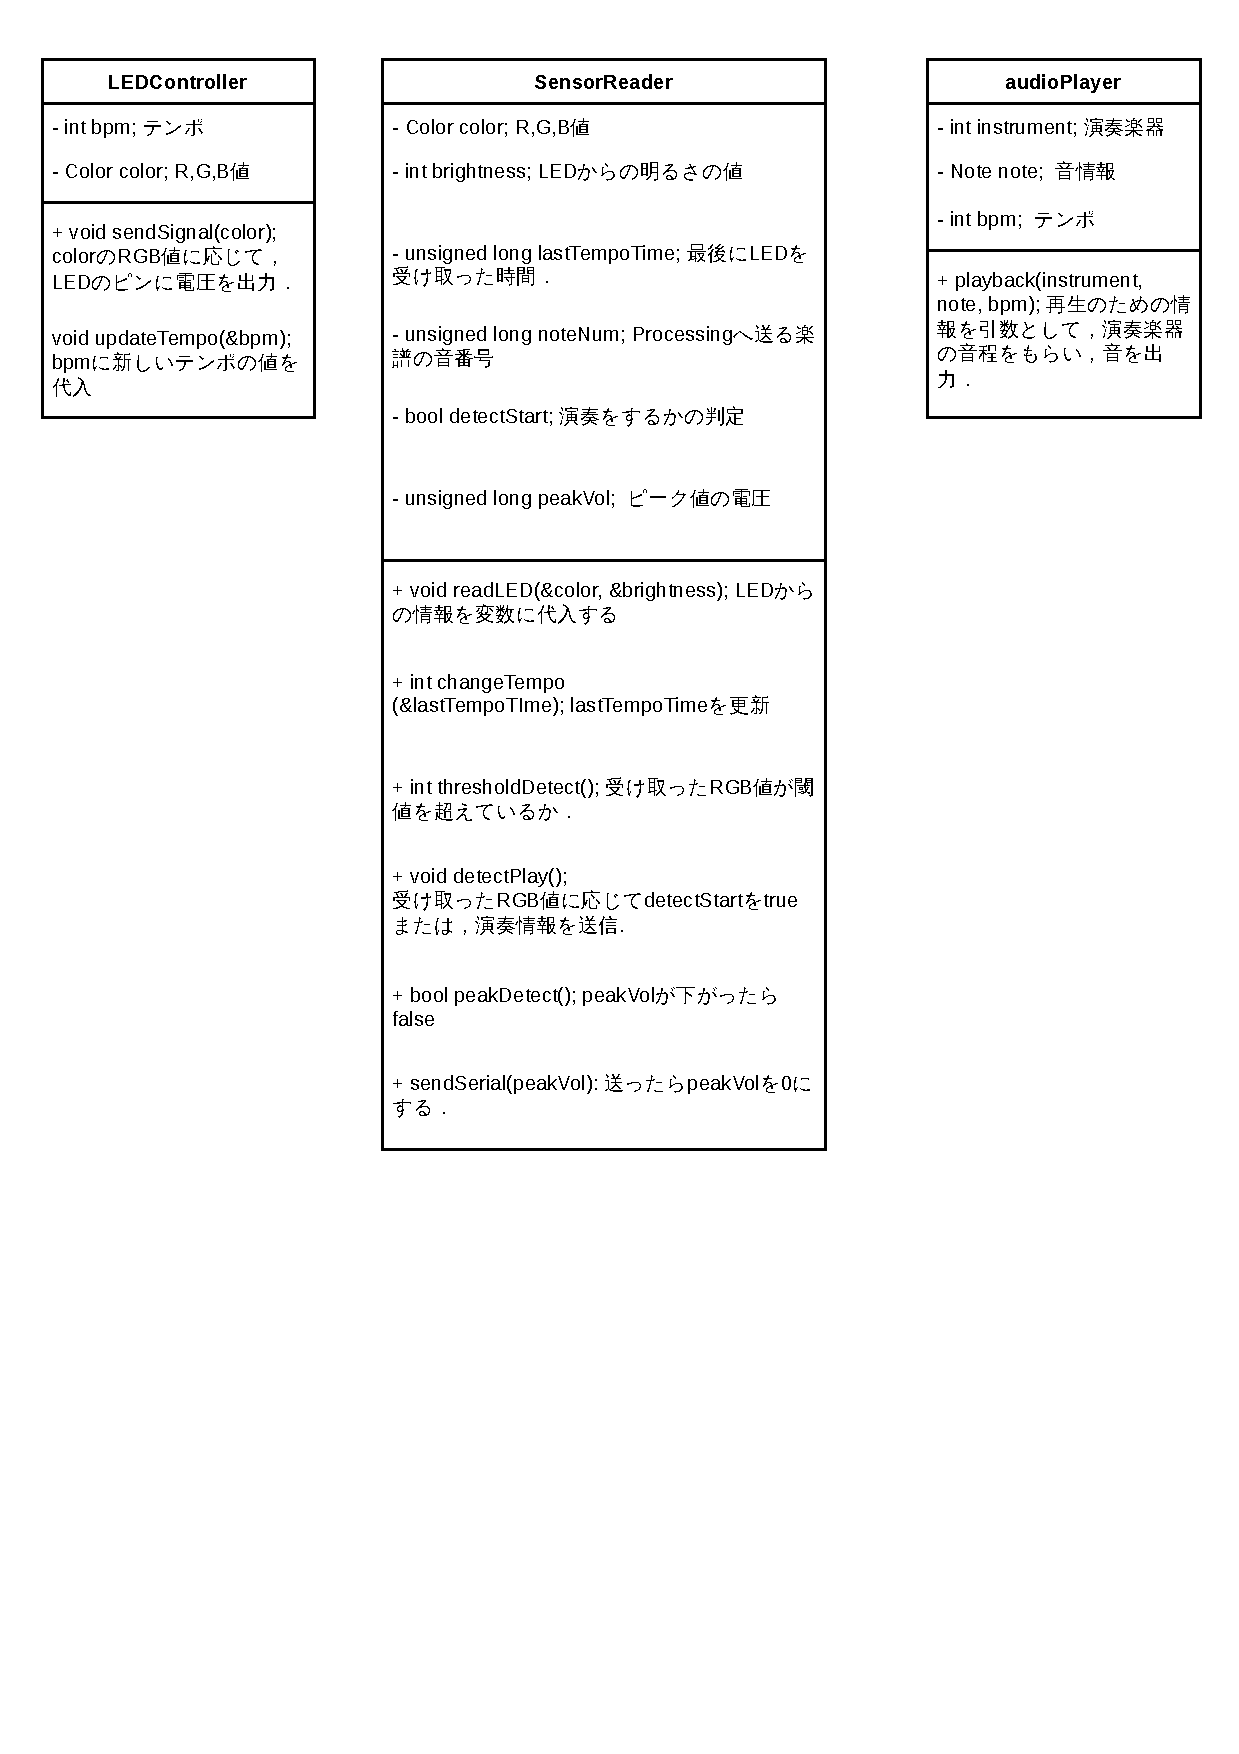
\includegraphics[width=140mm]{./img/class.pdf}
    \caption[gantt]{役割ごとのクラス図}
    \label{fig:class}
  \end{center}
\end{figure}

%%%%%%%%%%%%%%%%%%%%%%%%
\subsection{関数設計}
% 機能を分けた時に必要な関数と引数，内部処理，戻り値
% テンポ同期機能
% arduinoとProcessingでの送受信で必要な関数
% 音を鳴らすために必要な関数


%====================================================
% LED同期
%====================================================
\begin{table}[H]
  \centering
  \caption{LED同期関連の関数設計}
  \label{tab:led_sync}
  \scalebox{0.8}{
  \begin{tabular}{|p{3.5cm}|p{4cm}|p{2cm}|p{6cm}|}
    \hline
    関数名 & 引数 & 戻り値 & 処理 \\ \hline

    applyLED(c, level) &
    c : 点灯色, level : 輝度 &
    void &
    フルカラーLEDを指定した色・輝度で点灯させる．（conductor.ino） \\ \hline

    colorForPulse(pulseIdx) &
    pulseIdx : パルス番号 &
    LightColor &
    パルス番号に対応する点灯色を返す．（conductor.ino） \\ \hline

    detectColorID(r, g, b) &
    r, g, b : RGB値 &
    int &
    受信した色情報が自分の担当色と一致するか判定し，色IDを返す．一致しない場合は-1を返す．（playerRGBMethod.ino） \\ \hline

  \end{tabular}
  }
\end{table}



%====================================================
% シリアル通信
%====================================================
\begin{table}[H]
  \centering
  \caption{シリアル通信関連の関数設計}
  \label{tab:serial}
  \scalebox{0.8}{
  \begin{tabular}{|p{3.5cm}|p{4cm}|p{2cm}|p{6cm}|}
    \hline
    関数名 & 引数 & 戻り値 & 処理 \\ \hline

    sendNote() &
    なし &
    void &
    音高・音量・音長・楽器IDを32bitにパックしてシリアル通信で送信する．（playerRGBMethod.ino） \\ \hline

    serialEvent(p) &
    p : Serialオブジェクト &
    void &
    受信した4バイトをシフト演算で分解し，音高・音量・音長・楽器IDを変数へ格納する．（soundPlayer.pde） \\ \hline

  \end{tabular}
  }
\end{table}



%====================================================
% LEDマトリクス点滅
%====================================================
\begin{table}[H]
  \centering
  \caption{LEDマトリクス関連の関数設計}
  \label{tab:matrix}
  \scalebox{0.8}{
  \begin{tabular}{|p{3.5cm}|p{4cm}|p{2cm}|p{6cm}|}
    \hline
    関数名 & 引数 & 戻り値 & 処理 \\ \hline

    showBPM(bpm) &
    bpm : BPM値 &
    void &
    BPMの値を3桁の数字としてLEDマトリクスに表示する．（conductor.ino） \\ \hline

    drawDigit(bitmap, digit, xOffset) &
    bitmap : 描画バッファ, digit : 表示する数字, xOffset : X方向オフセット &
    void &
    LEDマトリクスの描画バッファに1桁の数字を書き込む．（conductor.ino） \\ \hline

  \end{tabular}
  }
\end{table}



%====================================================
% 音再生
%====================================================
\begin{table}[H]
  \centering
  \caption{音再生関連の関数設計}
  \label{tab:play}
  \scalebox{0.8}{
  \begin{tabular}{|p{3.5cm}|p{4cm}|p{2cm}|p{6cm}|}
    \hline
    関数名 & 引数 & 戻り値 & 処理 \\ \hline

    playNoteFromData(pi, vol, dur, inst) &
    pi : 音高, vol : 音量, dur : 音長, inst : 楽器ID &
    void &
    受信した音情報を基に，楽器IDに応じた音色で音を再生する．（soundPlayer.pde） \\ \hline

  \end{tabular}
  }
\end{table}

%====================================================
% Web通信
%====================================================
\begin{table}[H]
  \centering
  \caption{Web通信関連の関数設計}
  \label{tab:web}
  \scalebox{0.8}{
  \begin{tabular}{|p{3.5cm}|p{4cm}|p{2cm}|p{6cm}|}
    \hline
    関数名 & 引数 & 戻り値 & 処理 \\ \hline

    handleWebRequest() &
    なし &
    void &
    WebサーバーからのHTTPリクエストを受信し，BPM・音量・演奏開始停止等のパラメータを反映する．（conductor.ino / playerRGBMethod.ino） \\ \hline

    sendHeartbeat() &
    なし &
    void &
    サーバーへ定期的に登録リクエストを送信し，接続状態を維持する．（conductor.ino / playerRGBMethod.ino） \\ \hline

    tryReconnect() &
    なし &
    void &
    待機中にサーバーへの再登録を試み，成功した場合はWebサーバーを起動する．（conductor.ino / playerRGBMethod.ino） \\ \hline

    getWebParam(query, key) &
    query : クエリ文字列, key : パラメータ名 &
    int &
    クエリ文字列から指定キーの値を取り出す．存在しない場合は-1を返す．（conductor.ino / playerRGBMethod.ino） \\ \hline

    enterStandaloneMode() &
    なし &
    void &
    WiFiへの接続またはサーバーへの登録に失敗した場合に，WiFi無しの単体動作モードへ移行する．（conductor.ino） \\ \hline

  \end{tabular}
  }
\end{table}

%%%%%%%%%%%%%%%%%%%%%%%%
%%%%%%%%%%%%%%%%%%%%%%%%
\section{処理フローの設計}
% 関数を使用してどういった処理になるか

図\ref{fig:シーケンス}に本システム全体の
シーケンス図を示す．
本システムは指揮者Arduino，演奏者Arduino，
Processing，Webサイトの4つで
構成される．
WebサイトからBPM，全体音量，ループ，起動・停止信号を
指揮者Arduinoが受信し，LEDによる光信号として
演奏者Arduinoへ送信する．
また，楽器，楽譜，個別音量はWebサイトから演奏者Arduinoへ直接送信される．
演奏者Arduinoは光信号を受信・解析し，
Processingへ演奏情報を送信することで音の再生
および歌詞表示を行う．
なお，光信号を受信できない場合は待機状態を維持し，演奏を開始しない．
また，Webサイトから設定情報を受信できない場合は設定変更は行われない．

\begin{figure}[H]
  \begin{center}
    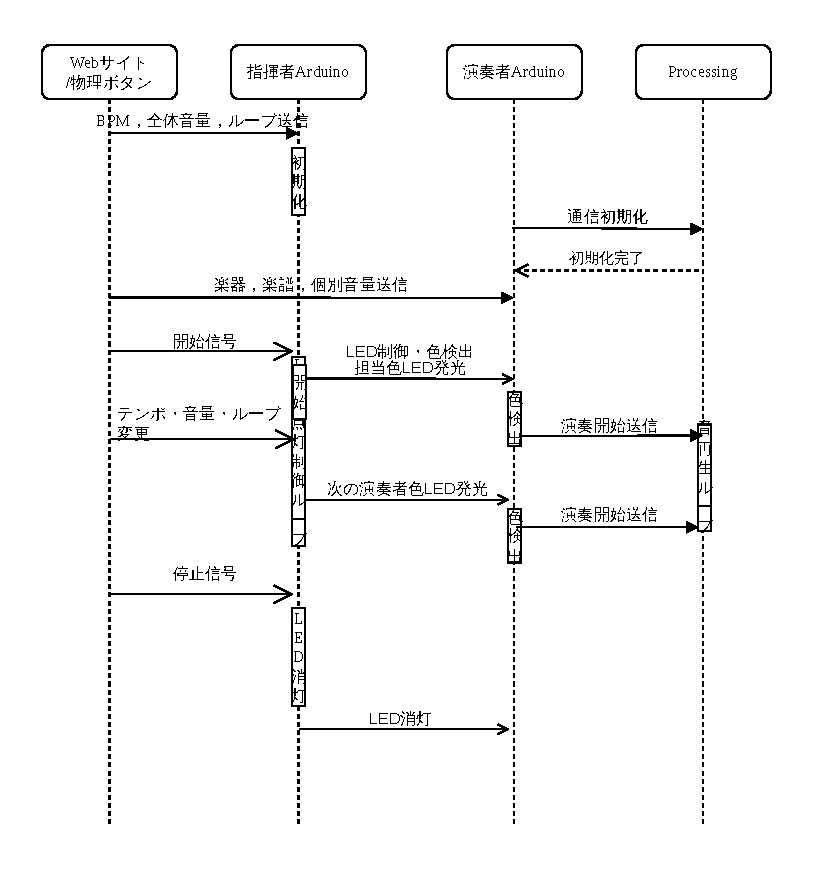
\includegraphics[width=80mm]{./img/シーケンス_6_26.pdf}
    \caption[シーケンス]{全体の処理のシーケンス図}
    \label{fig:シーケンス}
  \end{center}
\end{figure}





また，各構成要素間のやり取りの詳細について，
図\ref{fig:演奏者}，図\ref{fig:指揮者}，図\ref{fig:Web}に演奏者，指揮者，Webのそれぞれのフローチャートを示す．
演奏者は，起動後にProcessingとの通信を初期化し，担当楽器および担当色を確認する．
次に，WebサイトからHTTP通信によって楽器，楽譜，個別音量の情報を受信する．
その後，カラーセンサによる待機状態へ移行し，自身の担当色を検出した場合にProcessingへ演奏開始信号を送信し，音の再生を行う．
また，演奏開始後に3000\,ms以上LED点滅を検知できなかった場合は，演奏インデックスおよびフラグを初期化してカラーセンサ待機状態へリセットする．
停止ボタンが押下されると，Processingとの通信を終了し，処理を停止する．


指揮者側では，Webサイトとの通信確立後，BPM，全体音量，ループ，起動・停止信号の情報を受信する．
受信した情報をもとにLEDの点灯制御を行い，LEDを通じて各演奏者のArduinoへ
担当楽器のタイミングを共有する．
演奏中にテンポ，音量，ループの変更が行われた場合は設定を更新し，
停止信号を受信した時点で演奏を停止してLEDを消灯する．
輪唱の実装では，各パートの演奏開始タイミングを一定パルス数（OFFSET\_PULSES\_PER\_PART）だけずらすことで，パートごとに異なるタイミングで演奏が開始される仕組みとなっている．


Webサイトは，起動後，ユーザが演奏者ごとに楽器，楽譜，個別音量を設定するとともに，BPM，全体音量，ループを設定し，演奏開始ボタンを押下することで指揮者および演奏者へ演奏情報を送信する．
演奏中はテンポ，音量，ループの変更の有無を監視し，変更があった場合は随時情報を更新する．
演奏停止ボタンが押下された時点で処理を終了する．



\begin{figure}[H]
  \begin{center}
    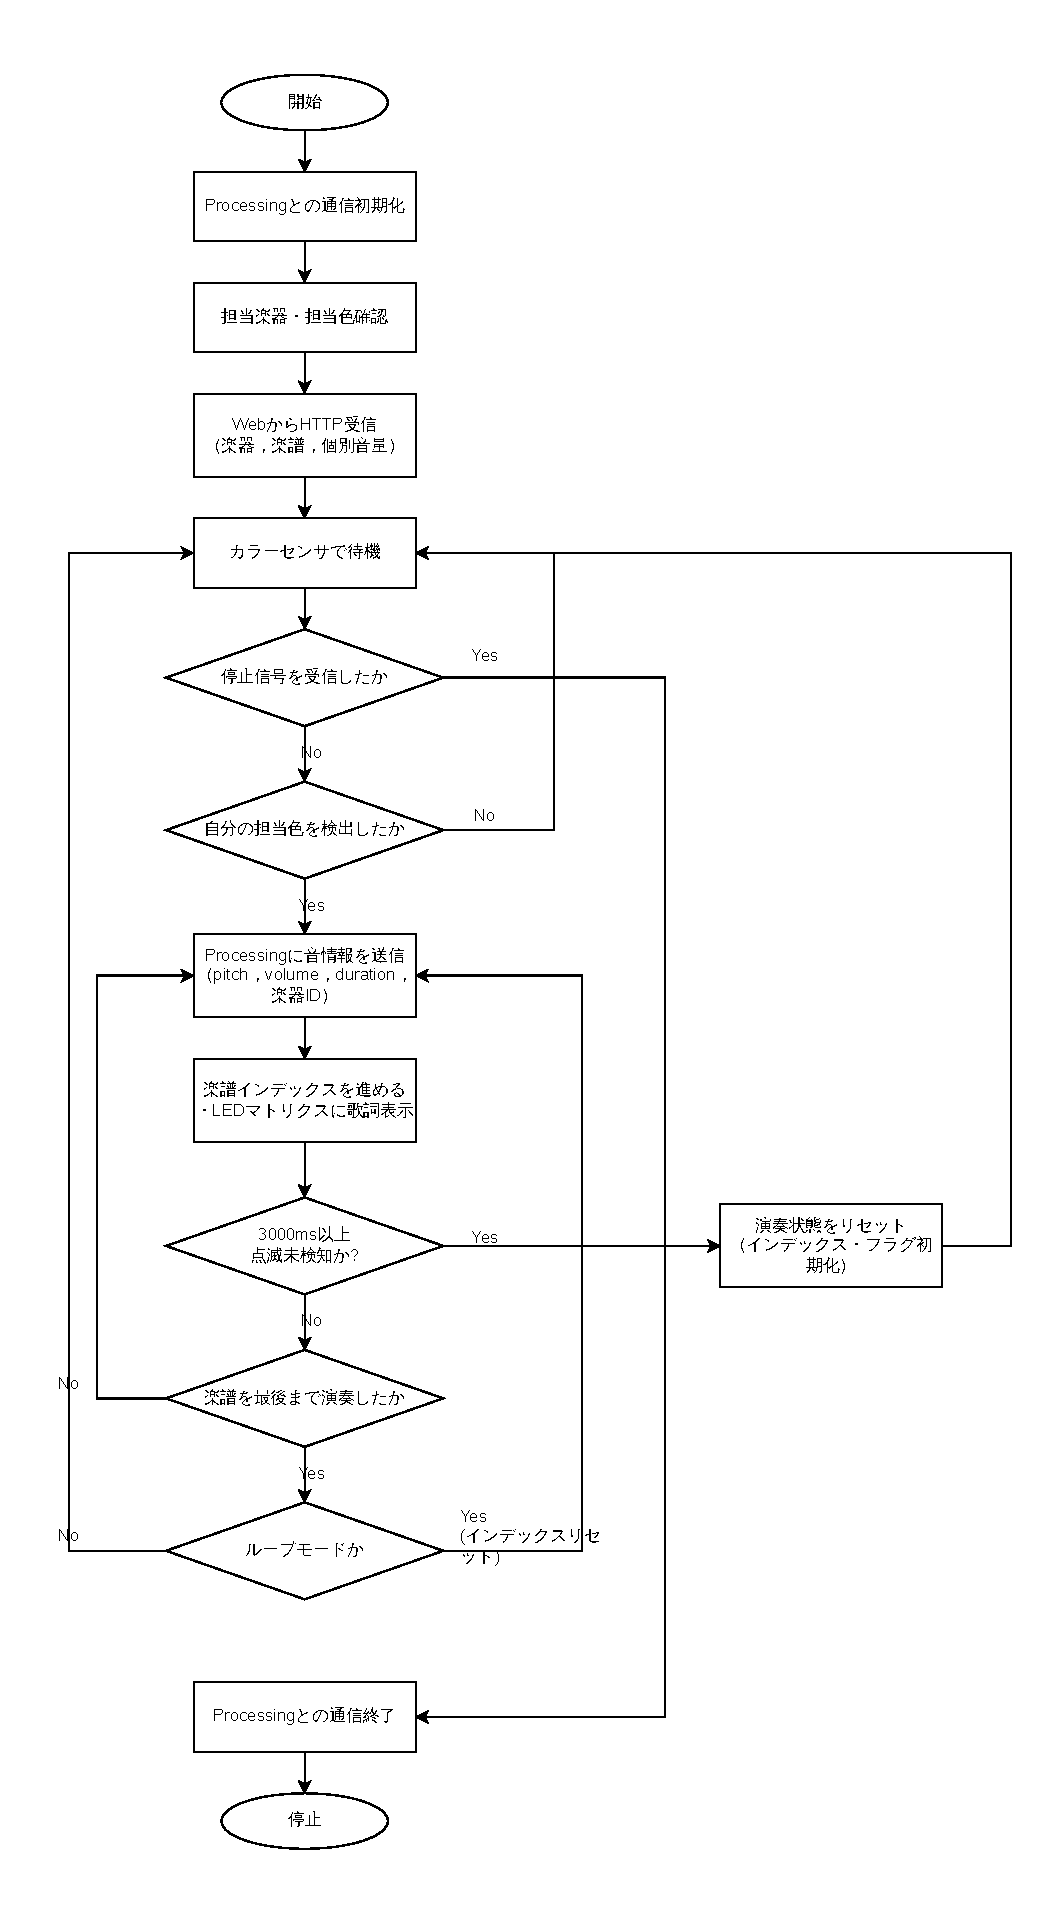
\includegraphics[width=60mm]{./img/playerFlowchar_7_3.pdf}
    \caption[演奏者]{演奏者側の全体のフローチャート}
    \label{fig:演奏者}
  \end{center}
\end{figure}



\begin{figure}[H]
  \begin{center}
    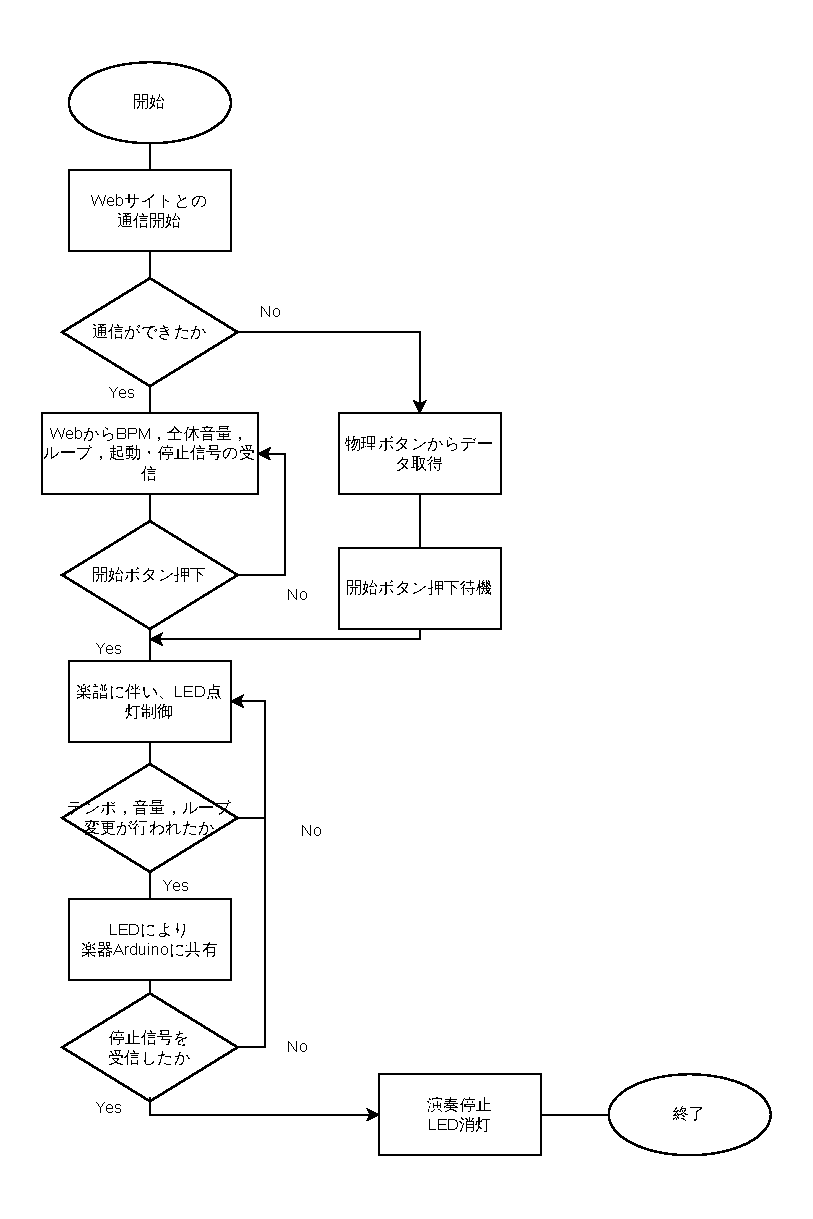
\includegraphics[width=140mm]{./img/指揮者フロー_6_26.pdf}
    \caption[指揮者]{指揮者側の全体のフローチャート}
    \label{fig:指揮者}
  \end{center}
\end{figure}

\begin{figure}[H]
  \begin{center}
    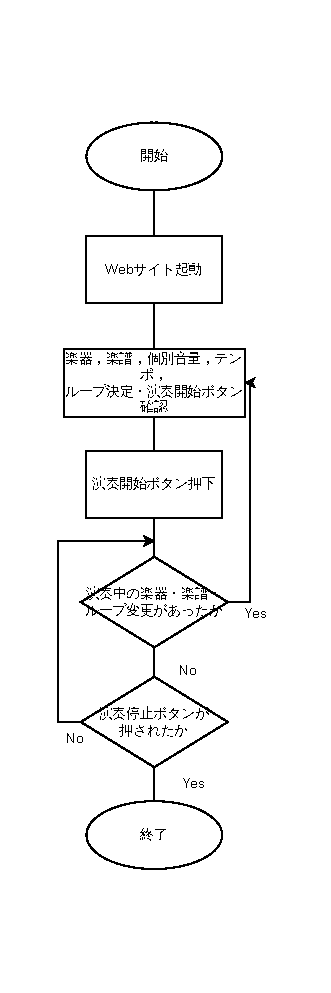
\includegraphics[width=70mm]{./img/Webフロー_6_26.pdf}
    \caption[Web]{Web関連の全体のフローチャート}
    \label{fig:Web}
  \end{center}
\end{figure}

%%%%%%%%%%%%%%%%%%%%%%%%
%%%%%%%%%%%%%%%%%%%%%%%%
\section{テストの設計}

%%%%%%%%%%%%%%%%%%%%%%%%
\subsection{システムテストの設計}

\subsubsection*{(1) 光と音の発生時間差}

スマートフォンまたはカメラのハイスピード撮影機能（240 fps等）を使用し，指揮者のLEDと演奏者PCのスピーカーが同一画面内に収まるよう動画を撮影する．
撮影した動画をPC上の動画編集ソフトに読み込み，LEDが発光したフレームから，スピーカーから音が出たフレームまでのフレーム数を計測し，時間差を算出する．

\subsubsection*{(2) 楽器間の同期ズレ}

(1)と同様に，ハイスピード撮影を用いて複数の演奏者PCのスピーカーを同一画面内に収めて撮影する．
撮影した動画から各演奏者の発音フレームを特定し，演奏者間のフレーム差を時間に換算して同期ズレを算出する．

\subsubsection*{(3) Webサイト送信〜演奏反映までの遅延}

以下の2種類の方法を併用して計測する．
\begin{itemize}
    \item \textbf{ハイスピード動画撮影による計測：}\\
    ハイスピード撮影機能を用いて，Webサイト画面と演奏者PCのスピーカーが同一画面内に収まるよう動画を撮影する．
    撮影した動画から，送信が実行されたフレームから音が変化したフレームまでのフレーム数を計測し，遅延時間を算出する．
    \item \textbf{ログによるシステム計測：}\\
    Webサイト側で送信が実行された瞬間のUNIXタイムスタンプ（ミリ秒単位）をログに記録する．
    同様に，演奏側プログラムにおいて，受信データの解析およびテンポ変数等の書き換え処理が完了した瞬間のタイムスタンプを記録する．
    両タイムスタンプの差分を遅延時間として算出する．
    なお，PC間で時計が同期していない場合はNTPによる時刻同期を行うか，同一PC上でテストを実施する．
\end{itemize}

%%%%%%%%%%%%%%%%%%%%%%%%
\subsection{結合テストの設計}

\subsubsection*{(1) 光同期のパケット損失率}
LEDを一定回数（2000回）発光させ，受信側の光センサが正しく検知できた回数および検知できなかった回数を目視により計数する．
発光回数（総パケット数）に対する検知失敗回数（損失パケット数）の割合をパケット損失率（IPLR）として算出する．

\subsubsection*{(2) Webサイトのパケット損失率}

Webサイトからテンポ変更や楽器指定などの制御コマンドを一定回数送信し，送信ログと受信ログを出力する．
両ログを比較し，総パケット数に対する損失パケット数の割合（パケット損失率／IPLR）を算出する．

%%%%%%%%%%%%%%%%%%%%%%%%
\subsection{単体テストの設計}

\subsubsection*{(1) 音色の再現性}

再現対象となる実際の楽器音の録音データと，本システムから出力された再現音の録音データをそれぞれ用意する．
比較の前処理として，両者の音量をRMS正規化により統一し，pYINアルゴリズムで推定したF0を用いて音程が一致していることを確認する．
その後，両者の音声波形データから，立ち上がり時間（AT），スペクトル重心（SC），スペクトル変動度（DSV），奇偶倍音比（OER）の4つの音色特徴量を算出する．
ATはRMSエンベロープのピーク到達時間，SCは持続区間（25〜75\%）のスペクトル重心周波数，DSVはフレーム間L2相対変化量の平均，OERはpYINで推定したF0を用いた$E_{\mathrm{odd}}/(E_{\mathrm{odd}}+E_{\mathrm{even}})$として算出する．
実際の楽器音と再現音の各特徴量を比較し，それぞれの目標差以内であることを確認する．
本テストは各楽器・音程ごとに実施し，全結果の平均を取り評価する．

また，音色の評価に関して，AT・SC・DSV・OER の 4 つの音色特徴量の算出の他にアンケートも同時に行う．
作成した回答用フォームを用いた音色評価を実施し，その結果を元に評価を行う．
この音色評価は，参加者に作成した音と実際の楽器の音を聞き比べてもらい，目的音をどの程度再現できているかを以下の5段階で評価してもらう形式とする．
\begin{itemize}
    \item 5,似ている
    \item 4,どちらかといえば似ている
    \item 3,どちらとも言えない
    \item 2,どちらかといえば似ていない
    \item 1,似ていない
\end{itemize}

この5段階評価の平均値を用いて評価する．
集計したものの平均が3.51以上の場合，同意と解釈して良いという先行研究\cite{アンケート}に基づき，集計結果の平均値が3.51以上の場合に十分に
音色を再現できたと評価する．

アンケートフォーム内には音色評価の他に，年代，音楽経験の有無，演奏環境についての質問も含まれる．
年齢を収集する理由は，回答者の聴覚特性の違いが音色評価に影響を与える可能性があるためである．


加齢に伴い高周波数帯域を中心とした聴覚特性の変化が生じることが示されており\cite{年齢}，これが楽器音のような複雑な音の音質・音色知覚や主観評価に影響を及ぼすと考えられる．したがって，評価データの偏りを防ぎ，年代ごとの知覚傾向を正しく分析するために年齢の項目を設けた．


音楽経験の有無を収集する理由は，音楽に関する知識や訓練経験の違いが音色評価に影響を与える可能性があるためである．
音楽経験者は楽器音に接する機会が多く，音色の特徴や違いを識別する能力が高いと考えられる．
一方で，音楽経験のない回答者は一般的な聴取者としての評価を行うため，両者の評価傾向に差が生じる可能性がある．
したがって，音楽経験の有無による評価傾向の違いを分析するために当該項目を設けた．


視聴環境を収集する理由は，再生機器の特性の違いが音色評価に影響を与える可能性があるためである．
イヤホン，ヘッドホン，PCスピーカ，スマートフォン内蔵スピーカなどの再生機器は周波数特性や音圧特性が異なり，同一の音源であっても聴取者が知覚する音質や音色が変化する場合がある．
したがって，視聴環境による評価結果への影響を分析し，必要に応じて評価結果の解釈に反映するために当該項目を設けた．

\begin{thebibliography}{9}

\bibitem{組み合わせ} 神田竜, 岩野成利, 片寄晴弘, 複数のモバイルデバイスを九十九神と見立てるインタラクティブメディアアート：九i九i九,情報処理学会論文誌, 53巻, 3号, p1061-1068.

\bibitem{遅延研究}亀川 徹, 4-3 演奏時における音声遅延の検知限とその影響, 映像情報メディア学会誌, 2015, 69 巻, 5 号, p. 408-411.

\bibitem{IoT}総務省, 情報通信白書令和2年版, 総務省, 2020, \url{https://www.soumu.go.jp/johotsusintokei/whitepaper/ja/r02/pdf/index.html}， 2026年4月21日参照.

\bibitem{視覚聴覚}Fada Pan, Li Zhang, Yuhong Ou, and Xinni Zhang, "Audiovisual integration effect on music emotion: Behavioral and physiological evidence," PLoS ONE, Vol. 14, No. 5, p. e0217040, 2019.

\bibitem{無線} 新 誠一, 計測制御のための無線通信技術の現状と展望, 計測と制御, 2009, 48 巻, 7 号, p. 537-541．

\bibitem{光無線通信} 若森 和彦, 光無線通信と画像伝送, 画像電子学会誌, 2011, 40 巻, 1 号, p. 257-263.

\bibitem{1998}International Telecommunication Union, [Recommendation] Relative timing of sound and vision for broadcasting (Recommendation ITU-R BT.1359-1), ITU Radiocommunication Assembly, 1998.

\bibitem{brown}A. D. Brown, G. C. Stecker, D. J. Tollin, "The Precedence Effect in Sound Localization," Journal of the Association for Research in Otolaryngology, Vol. 16, No. 1, pp. 1-28, 2015.

\bibitem{1968}R. B. Miller, "Response time in man-computer conversational transactions," in Proceedings of the AFIPS Fall Joint Computer Conference, Vol. 33, pp. 267-277, 1968.

\bibitem{1541}International Telecommunication Union, "Network performance objectives for IP-based services," ITU-T Recommendation Y.1541, 2011.

\bibitem{McAdams}S. McAdams, S. Winsberg, S. Donnadieu, G. De Soete, J. Krimphoff, "Perceptual scaling of synthesized musical timbres: Common dimensions, specificities, and latent subject classes," Psychological Research, Vol. 58, No. 3, pp. 177-192, 1995.

\bibitem{Siedenburg}K. Siedenburg, "Timbral and dynamic differentiability of musical instrument tones," The Journal of the Acoustical Society of America, Vol. 145, No. 2, pp. 1078-1087, 2019.

\bibitem{Wun}C. Wun, A. Horner, C. Wu, "Timbre discrimination of musical instruments in melody," Journal of the Audio Engineering Society, Vol. 62, No. 9, pp. 575-583, 2014.

\bibitem{Horner}A. Horner, J. Beauchamp, R. So, "Detection of random spectral variation in musical instrument sounds," The Journal of the Acoustical Society of America, Vol. 116, No. 3, pp. 1800-1810, 2004.

\bibitem{pyin}M. Mauch and S. Dixon, "pYIN: A fundamental frequency estimator using probabilistic threshold distributions," in Proc. IEEE International Conference on Acoustics, Speech and Signal Processing (ICASSP), pp. 659-663, 2014.

\bibitem{Caclin}A. Caclin, S. McAdams, B. K. Smith, S. Winsberg, "Acoustic correlates of timbre space dimensions: A confirmatory study using synthetic tones," The Journal of the Acoustical Society of America, Vol. 118, No. 1, pp. 471-482, 2005.

\bibitem{McAdams}S. McAdams, S. Winsberg, S. Donnadieu, G. De Soete, J. Krimphoff, "Perceptual scaling of synthesized musical timbres: Common dimensions, specificities, and latent subject classes," Psychological Research, Vol. 58, No. 3, pp. 177-192, 1995.

\bibitem{アンケート} J. R. Lindner, N. J. Lindner, "Interpreting Likert-type Scales, Summated Scales, Unidimensional Scales, and Attitudinal Scales: I neither Agree nor Disagree, Likert or Not," Advancements in Agricultural Development, Vol. 5, No. 2, 2024.

\bibitem{年齢} 入野 俊夫, 加齢性難聴の模擬による聴覚特性理解へのアプローチ, 日本音響学会誌, 2025, 81 巻, 5 号, p. 352-359.

\end{thebibliography}
\end{document}